\documentclass[a4paper,11pt,twoside]{report}
\usepackage[left=2.5cm,right=2cm,top=2cm,bottom=2cm]{geometry}

\usepackage{times}
\usepackage{graphicx}
\usepackage{epsfig}
\usepackage{amssymb}
\usepackage{amsmath}
\usepackage{amsfonts}
\usepackage{amsthm}
\usepackage{epstopdf}
\usepackage{url}
\usepackage{amsmath}
\usepackage{mathtools}
\usepackage{fixltx2e}
\usepackage{parskip}
\usepackage{framed}
\usepackage{enumitem}
\usepackage{amssymb}
\usepackage{algorithm}
\usepackage{algpseudocode}
\usepackage{framed}
\usepackage{caption}

\newcommand{\HRule}{\rule{\linewidth}{0.4mm}}
\newcommand{\tab}[1]{\hspace{.08\textwidth}{#1}} % indent tab for data
% structs in algos
% THIS IS PRETTY SPECIFICS FOR 
% THE CASE BELOW SO MAYBE DONT 
% WORRY ABOUT IT
\newcommand{\LineIf}[3]{ {#1}
  \algorithmicif\ {#2}
  \algorithmicelse\ {#3} } % inline X if Y else Z !!!ZOMG

\usepackage{graphicx}
\usepackage{verbatim}
\usepackage{latexsym}
\usepackage{mathchars}
\usepackage{setspace}

\setlength{\parskip}{\medskipamount}  % a little space before a \par
\setlength{\parindent}{0pt}	      % don't indent first lines of paragraphs
%UHEAD.STY  If this is included after \documentstyle{report}, it adds
% an underlined heading style to the LaTeX report style.
% \pagestyle{uheadings} will put underlined headings at the top
% of each page. The right page headings are the Chapter titles and
% the left page titles are supplied by \def\lefthead{text}.

% Ted Shapin, Dec. 17, 1986

\makeatletter
\def\chapapp2{Chapter}

\def\appendix{\par
 \setcounter{chapter}{0}
 \setcounter{section}{0}
 \def\chapapp2{Appendix}
 \def\@chapapp{Appendix}
 \def\thechapter{\Alph{chapter}}}

\def\ps@uheadings{\let\@mkboth\markboth
% modifications
\def\@oddhead{\protect\underline{\protect\makebox[\textwidth][l]
		{\sl\rightmark\hfill\rm\thepage}}}
\def\@oddfoot{}
\def\@evenfoot{}
\def\@evenhead{\protect\underline{\protect\makebox[\textwidth][l]
		{\rm\thepage\hfill\sl\leftmark}}}
% end of modifications
\def\chaptermark##1{\markboth {\ifnum \c@secnumdepth >\m@ne
 \chapapp2\ \thechapter. \ \fi ##1}{}}%
\def\sectionmark##1{\markright {\ifnum \c@secnumdepth >\z@
   \thesection. \ \fi ##1}}}
\makeatother
%%From: marcel@cs.caltech.edu (Marcel van der Goot)
%%Newsgroups: comp.text.tex
%%Subject: illegal modification of boxit.sty
%%Date: 28 Feb 92 01:10:02 GMT
%%Organization: California Institute of Technology (CS dept)
%%Nntp-Posting-Host: andromeda.cs.caltech.edu
%%
%%
%%Quite some time ago I posted a file boxit.sty; maybe it made it
%%to some archives, although I don't recall submitting it. It defines
%%	\begin{boxit}
%%	...
%%	\end{boxit}
%%to draw a box around `...', where the `...' can contain other
%%environments (e.g., a verbatim environment). Unfortunately, it had
%%a problem: it did not work if you used it in paragraph mode, i.e., it
%%only worked if there was an empty line in front of \begin{boxit}.
%%Luckily, that is easily corrected.
%%
%%HOWEVER, apparently someone noticed the problem, tried to correct it,
%%and then distributed this modified version. That would be fine with me,
%%except that:
%%1. There was no note in the file about this modification, it only has my
%%   name in it.
%%2. The modification is wrong: now it only works if there is *no* empty
%%   line in front of \begin{boxit}. In my opinion this bug is worse than
%%   the original one.
%%
%%In particular, the author of this modification tried to force an empty
%%line by inserting a `\\' in the definition of \Beginboxit. If you have
%%a version of boxit.sty with a `\\', please delete it. If you have my
%%old version of boxit.sty, please also delete it. Below is an improved
%%version.
%%
%%Thanks to Joe Armstrong for drawing my attention to the bug and to the
%%illegal version.
%%
%%                                          Marcel van der Goot
%% .---------------------------------------------------------------
%% | Blauw de viooltjes,                    marcel@cs.caltech.edu
%% |    Rood zijn de rozen;
%% | Een rijm kan gezet
%% |    Met plaksel en dozen.
%% |


% boxit.sty
% version: 27 Feb 1992
%
% Defines a boxit environment, which draws lines around its contents.
% Usage:
%   \begin{boxit}
%	... (text you want to be boxed, can contain other environments)
%   \end{boxit}
%
% The width of the box is the width of the contents.
% The boxit* environment behaves the same, except that the box will be
% at least as wide as a normal paragraph.
%
% The reason for writing it this way (rather than with the \boxit#1 macro
% from the TeXbook), is that now you can box verbatim text, as in
%   \begin{boxit}
%   \begin{verbatim}
%   this better come out in boxed verbatim mode ...
%   \end{verbatim}
%   \end{boxit}
%
%						Marcel van der Goot
%						marcel@cs.caltech.edu
%

\def\Beginboxit
   {\par
    \vbox\bgroup
	   \hrule
	   \hbox\bgroup
		  \vrule \kern1.2pt %
		  \vbox\bgroup\kern1.2pt
   }

\def\Endboxit{%
			      \kern1.2pt
		       \egroup
		  \kern1.2pt\vrule
		\egroup
	   \hrule
	 \egroup
   }	

\newenvironment{boxit}{\Beginboxit}{\Endboxit}
\newenvironment{boxit*}{\Beginboxit\hbox to\hsize{}}{\Endboxit}
\pagestyle{empty}

\setlength{\parskip}{2ex plus 0.5ex minus 0.2ex}
\setlength{\parindent}{0pt}

\makeatletter  %to avoid error messages generated by "\@". Makes Latex treat "@" like a letter

\linespread{1.5}
\def\submitdate#1{\gdef\@submitdate{#1}}

\def\maketitle{
  \begin{titlepage}{
    %\linespread{1.5}
    \Large University of London \\
    %\linebreak
    Imperial College of Science, Technology and Medicine \\
    %\linebreak
    Department of Computing
    \rm
    \vskip 3in
    \Large \bf \@title \par
  }
  \vskip 0.3in
  \par
  {\Large \@author}
  \vskip 4in
  \par
  Submitted in part fulfilment of the requirements for the degree of 
  \linebreak
  Doctor of Philosophy in Computing of the University of London and 
  \linebreak
  the Diploma of Imperial College, \@submitdate
  \vfil
  \end{titlepage}
}

\def\titlepage{
  \newpage
  \centering
  \linespread{1}
  \normalsize
  \vbox to \vsize\bgroup\vbox to 9in\bgroup
}
\def\endtitlepage{
  \par
  \kern 0pt
  \egroup
  \vss
  \egroup
  \cleardoublepage
}

\def\abstract{
  \begin{center}{
    \large\bf Abstract}
  \end{center}
  \small
  %\def\baselinestretch{1.5}
  \linespread{1.5}
  \normalsize
}
\def\endabstract{
  \par
}

\newenvironment{acknowledgements}{
  \cleardoublepage
  \begin{center}{
    \large \bf Acknowledgements}
  \end{center}
  \small
  \linespread{1.5}
  \normalsize
}{\cleardoublepage}
\def\endacknowledgements{
  \par
}

\newenvironment{dedication}{
  \cleardoublepage
  \begin{center}{
    \large \bf Dedication}
  \end{center}
  \small
  \linespread{1.5}
  \normalsize
}{\cleardoublepage}
\def\enddedication{
  \par
}

\def\preface{
    \pagenumbering{roman}
    \pagestyle{plain}
    \doublespacing
}

\def\body{
    \cleardoublepage    
    \pagestyle{uheadings}
    \tableofcontents
    \pagestyle{plain}
    \cleardoublepage
    \pagestyle{uheadings}
    \listoftables
    \pagestyle{plain}
    \cleardoublepage
    \pagestyle{uheadings}
    \listoffigures
    \pagestyle{plain}
    \cleardoublepage
    \pagestyle{uheadings}
    \pagenumbering{arabic}
    \doublespacing
}

\makeatother  %to avoid error messages generated by "\@". Makes Latex treat "@" like a letter

\newcommand{\ipc}{{\sf ipc}}

\newcommand{\Prob}{\bbbp}
\newcommand{\Real}{\bbbr}
\newcommand{\real}{\Real}
\newcommand{\Int}{\bbbz}
\newcommand{\Nat}{\bbbn}

\newcommand{\NN}{{\sf I\kern-0.14emN}}   % Natural numbers
\newcommand{\ZZ}{{\sf Z\kern-0.45emZ}}   % Integers
\newcommand{\QQQ}{{\sf C\kern-0.48emQ}}   % Rational numbers
\newcommand{\RR}{{\sf I\kern-0.14emR}}   % Real numbers
\newcommand{\KK}{{\cal K}}
\newcommand{\OO}{{\cal O}}
\newcommand{\AAA}{{\bf A}}
\newcommand{\HH}{{\bf H}}
\newcommand{\II}{{\bf I}}
\newcommand{\LL}{{\bf L}}
\newcommand{\PP}{{\bf P}}
\newcommand{\PPprime}{{\bf P'}}
\newcommand{\QQ}{{\bf Q}}
\newcommand{\UU}{{\bf U}}
\newcommand{\UUprime}{{\bf U'}}
\newcommand{\zzero}{{\bf 0}}
\newcommand{\ppi}{\mbox{\boldmath $\pi$}}
\newcommand{\aalph}{\mbox{\boldmath $\alpha$}}
\newcommand{\bb}{{\bf b}}
\newcommand{\ee}{{\bf e}}
\newcommand{\mmu}{\mbox{\boldmath $\mu$}}
\newcommand{\vv}{{\bf v}}
\newcommand{\xx}{{\bf x}}
\newcommand{\yy}{{\bf y}}
\newcommand{\zz}{{\bf z}}
\newcommand{\oomeg}{\mbox{\boldmath $\omega$}}
\newcommand{\res}{{\bf res}}
\newcommand{\cchi}{{\mbox{\raisebox{.4ex}{$\chi$}}}}
%\newcommand{\cchi}{{\cal X}}
%\newcommand{\cchi}{\mbox{\Large $\chi$}}

% Logical operators and symbols
\newcommand{\imply}{\Rightarrow}
\newcommand{\bimply}{\Leftrightarrow}
\newcommand{\union}{\cup}
\newcommand{\intersect}{\cap}
\newcommand{\boolor}{\vee}
\newcommand{\booland}{\wedge}
\newcommand{\boolimply}{\imply}
\newcommand{\boolbimply}{\bimply}
\newcommand{\boolnot}{\neg}
\newcommand{\boolsat}{\!\models}
\newcommand{\boolnsat}{\!\not\models}


\newcommand{\op}[1]{\mathrm{#1}}
\newcommand{\s}[1]{\ensuremath{\mathcal #1}}

% Properly styled differentiation and integration operators
\newcommand{\diff}[1]{\mathrm{\frac{d}{d\mathit{#1}}}}
\newcommand{\diffII}[1]{\mathrm{\frac{d^2}{d\mathit{#1}^2}}}
\newcommand{\intg}[4]{\int_{#3}^{#4} #1 \, \mathrm{d}#2}
\newcommand{\intgd}[4]{\int\!\!\!\!\int_{#4} #1 \, \mathrm{d}#2 \, \mathrm{d}#3}

% Large () brackets on different lines of an eqnarray environment
\newcommand{\Leftbrace}[1]{\left(\raisebox{0mm}[#1][#1]{}\right.}
\newcommand{\Rightbrace}[1]{\left.\raisebox{0mm}[#1][#1]{}\right)}

% Funky symobols for footnotes
\newcommand{\symbolfootnote}{\renewcommand{\thefootnote}{\fnsymbol{footnote}}}
% now add \symbolfootnote to the beginning of the document...

\newcommand{\normallinespacing}{\renewcommand{\baselinestretch}{1.5} \normalsize}
\newcommand{\mediumlinespacing}{\renewcommand{\baselinestretch}{1.2} \normalsize}
\newcommand{\narrowlinespacing}{\renewcommand{\baselinestretch}{1.0} \normalsize}
\newcommand{\bump}{\noalign{\vspace*{\doublerulesep}}}
\newcommand{\cell}{\multicolumn{1}{}{}}
\newcommand{\spann}{\mbox{span}}
\newcommand{\diagg}{\mbox{diag}}
\newcommand{\modd}{\mbox{mod}}
\newcommand{\minn}{\mbox{min}}
\newcommand{\andd}{\mbox{and}}
\newcommand{\forr}{\mbox{for}}
\newcommand{\EE}{\mbox{E}}

\newcommand{\deff}{\stackrel{\mathrm{def}}{=}}
\newcommand{\syncc}{~\stackrel{\textstyle \rhd\kern-0.57em\lhd}{\scriptstyle L}~}

\def\coop{\mbox{\large $\rhd\!\!\!\lhd$}}
\newcommand{\sync}[1]{\raisebox{-1.0ex}{$\;\stackrel{\coop}{\scriptscriptstyle
#1}\,$}}

\newtheorem{definition}{Definition}[chapter]
\newtheorem{theorem}{Theorem}[chapter]

\newcommand{\Figref}[1]{Figure~\ref{#1}}
\newcommand{\fig}[3]{
 \begin{figure}[!ht]
 \begin{center}
 \scalebox{#3}{\includegraphics{figs/#1.ps}}
 \vspace{-0.1in}
 \caption[ ]{\label{#1} #2}
 \end{center}
 \end{figure}
}

\newcommand{\figtwo}[8]{
 \begin{figure}
 \parbox[b]{#4 \textwidth}{
 \begin{center}
 \scalebox{#3}{\includegraphics{figs/#1.ps}}
 \vspace{-0.1in}
 \caption{\label{#1}#2}
 \end{center}
 }
 \hfill
 \parbox[b]{#8 \textwidth}{
 \begin{center}
 \scalebox{#7}{\includegraphics{figs/#5.ps}}
 \vspace{-0.1in}
 \caption{\label{#5}#6}
 \end{center}
 }
 \end{figure}
}


\begin{document}
\begin{titlepage}
\begin{center}
	\textsc{\LARGE Imperial College London}\\[1.5cm]

	\textsc{\Large Department of Computing}\\[0.5cm]

	\HRule \\[0.4cm]
	{\LARGE \bfseries On-the-fly Modelling and Prediction of Epidemic Phenomena \\[0.4cm] }
	\HRule \\[1.5cm]

\begin{minipage}{0.4\textwidth}
\begin{flushleft} \large
\emph{Author:}\\
James \textsc{Hay}
\end{flushleft}
\end{minipage}
\begin{minipage}{0.4\textwidth}
\begin{flushright} \large
\emph{Supervisor:} \\
Dr.~William \textsc{Knottenbelt}
\end{flushright}
\end{minipage}
\vfill

\includegraphics[width=5cm]{ImperialCrest.jpg}
\vfill
Submitted in partial fulfilment of the requirements for the MSc Degree in Computing Science of Imperial College London
\vfill
% Bottom of the page
{\large September 2014}
\end{center}
\end{titlepage}


\preface
\addcontentsline{toc}{chapter}{Abstract}

\begin{abstract}

Text of the Abstract.

\end{abstract}
\cleardoublepage

\addcontentsline{toc}{chapter}{Acknowledgements}

\begin{acknowledgements}

I would like to express (whatever feelings I have) to:

\begin{itemize}
 \item My supervisor
 \vspace*{3mm}
 \item My second supervisor
 \vspace*{3mm}
 \item Other researchers
 \vspace*{3mm}
 \item My family and friends
\end{itemize}

\end{acknowledgements}
\cleardoublepage

\begin{dedication}
  Dedication here.
\end{dedication}
\clearpage

\narrowlinespacing

\vspace*{4mm}

`Quote text here.'\\
\\
\emph{Guy Quoted}

\normallinespacing

\body
\chapter{Introduction}
\section{Overview}
This project provides a framework with which the dynamics of
an epidemic event composed of multiple, overlapping sub-epidemics may be modelled and
forecasted in real time. We aim to provide an optimised model fit to a
given set of epidemic data where all model parameters are assumed to
be unknown. The challenge of considering various candidate model
types is also considered. Unlike previous approaches, the presented framework is
implemented in object oriented style using a general purpose
programming language, allowing improved customisability and
speed. Furthermore, we attempt to implement a maximum likelihood based
fitting procedure, which has previously only been considered for
single epidemic models.

\section{Motivation}
Epidemic spreading processes can be observed in a wide range of
fields. Any type of interaction between individuals will allow the
propogation of ideas or parasites through a population, with some spreading
processes arising unexpectedly in excess of baackground levels. In the case of
infectious diseases, such outbreaks are termed epidemics. Indeed, many significant
historical events have been heavily influenced by epidemics, and the
WHO estimates that infectious diseases account for more than 13
million deaths per year.\cite{who} It is therefore no wonder that
epidemiology, the study of the mechanisms and population dynamics of
infectious diseases, has become a central field of research. With the
advancement of computing technology and methodology, new opportunities
to develop complex mathematical and computational models of real-time
epidemics have emerged.

Although the study of infectious disease spread continues to be an
area of particular research focus, globalisation and advances in
communication technologies have led to a new and rapidly developing
type of internet based epidemic. With the entire world connected
online, new ideas, trends and information can disseminate through the
world wide web almost instantaneously, and as these spreading
processes become increasingly central to modern day life, interest
from academic, commercial and social fields continues to increase. One
highly relevant theory is that of `memes' as proposed by Richard
Dawkins, who suggests that ideas, behaviours and styles spread like
"mind viruses" between individuals within a culture.\cite{dawkins} The
adaptation of this term to describe the spread of fads on the internet
demonstrates the relevance of studying the dynamics of epidemic
processes over the internet. \cite{meme}

Research into the dynamics of internet-based phenomena are largely at
an early stage, and have mostly focused on Online Social Networks
(OSNs) such as Facebook and Twitter, and content sharing websites such
as YouTube.\cite{hartmann, bieber} The analogy between infectious
diseases and the spread of content online is easy to consider: the
social networks formed on OSNs simulate physical interactions in real
life as users interact and share content on their profiles, whilst
viewing and subsequently sharing a YouTube video may be compared to
contracting and spreading an infectious disease. There is a growing
body of research that aims to use ideas from epidemiology to better
understand the spread of internet-based phenomena. \cite{marily2013,
  meme, wang} Taking inspiration from epidemiology, the study of
internet-based epidemic phenomena has investigated the applicability
of both locally and globally driven models. For example, some studies
have investigated the use of diffusion models to describe the
disemmination of influence, whilst others have investigated the use of
global mathematical models.\cite{marily2013, meme, wang, hu}

Whilst these studies have shown generally promising results, a recent
study highlighted the limitations of the single epidemic based
approach.\cite{marily2013} The co-occurence and interaction between
diseases and with environmental factors is increasingly realised as
important, and the authors suggest that the corresponding field of
\emph{synepidemiology} can be applied to internet-based
epidemics.\cite{singer, bastos} The authors go on to coin the term
\emph{synthedemics} to describe the co-occurence of a set of
infections that may or may not be dependent on each
other.\cite{marily2014} Taking inspiration from Fourier analysis, the
study goes on to investigate how an incoming epidemic signal can be
broken down and described in terms of multiple epidemic components
(Figure 1). Furthermore, the authors build on a previous study to
allow models to be fit in real time without making assumptions
regarding the initial model parameters.




 \begin{figure}[ht!]
\centering
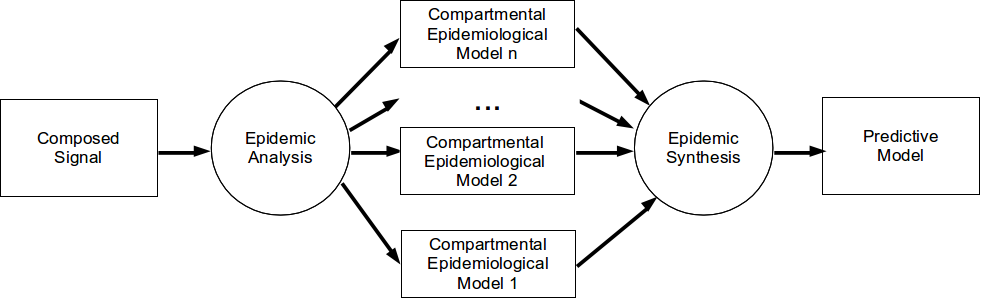
\includegraphics[width=140mm]{marily2014.png}
\caption{Model construction framework as proposed by Nika et al. 2014.\cite{marily2014}}
\label{sir}
\end{figure}

\section{Objectives}
The aim of this project is to implement a real time model fitting
framework with which epidemic phenomena might be characterised and
forecasted. When provided with epidemic data up to an arbritary time point,
we attempt to fit an appropriate number of sub-epidemics of various
types to best describe the current data, and to allow future time
points to be predicted. The course of the project can be split up into
the following sub goals:

\subsection{Single Epidemics}
The first objective of this project is to implement a single epidemic
fitting framework, treating the growth and recovery rates of the
epidemic as unknown parameters. This framework is then extended to
additionally consider the initial number of susceptible individuals
and the actual epidemic start time as unknown parameters. The model
fitting procedure is undertaken using optimisation with both least
squares and maximum likelihood estimations. The framework allows for
`on the fly' fitting, such that a model may be fit to the data as the
epidemic unfolds and more data points are obtained.

The initial implementation of this framework is initially undetaken using the R
statistics programming environment due to the availability of useful
packages and functions. For example, the \emph{deSolve} for solving
first-order ordinary differential equations (ODEs), the \emph{optim}
function for optimising a set of model parameters, and the
\emph{bbmle} package for maximum likeliihood based fitting.

An extension of this objective that arose during the course of the
project is the implementation of the fitting framework in C++ `from
scratch'.

\subsection{Multiple Epidemics}
Not all epidemic phenomena are constrained to a single population, and
the single epidemic fitting methodology is therefore inadequate in
characterising all epidemics. For example, the measure of
\emph{YouTube} video views over time might be composed of multiple
spikes of interest as the video is shared in new online social
groups. This limitation also affects to infectious disease dynamics,
wherein the total number of infected individuals in a country might be
affected by the penetration of the disease into different cities. The
second objective of this project is therefore to implement a model
fitting framework that can simultaneously fit and combine multiple
sub epidemics into a single model. 

As in the single epidemic fitting framework, the multiple epidemic
fitting framework makes no assumptions regarding model parameters such
as growth rate, recovery rate, start time and number of
susceptibles. As above, an initial implementation will be attempted
using R. However, as the computational difficulty of fitting
multiple sets of parameters simultaneously increases as the number of
sub epidemics increases. We therefore provide a final `from scratch' implementation in C++.

A significant extension of this fitting methodology is to allow
different epidemic models to be considered. That is, which one of a
number of model equations can be used to best describe the data? An
object-oriented C++ implementation is therefore provided to consider
the addition and removal of various candidate models to describe a set
of data.

\subsection{Maximum Likelihood Estimation}
A novel objective of this project is to use maximum likelihood rather
than least squares to find an optimised model fit. A significant
challenge of this is to implement an efficient likelihood function in
C++ with which a set of parameters might be optimised in reasonable
time. An advanced extension of this objective is to generate confidence
intervals characterise uncertainty in the optimised parameters. 

\subsection{Evaluation}
All of the above objectives must be validated, and we use a
number of data sources to assess the model fitting
framework. Synthetic data provides the core of the evaluation, as it
allows for the retrieval of known parameters from artificially
generated data. Finally, we consider the framework's ability to
provide model fits to historic infectious disease data and online
epidemic phenomena.

\section{Contributions}

Contributions here.


\section{Report Structure}

Statement here.

\chapter{Background Theory}

\label{ch:background}

\section{Modelling Infectious Disease Dynamics}
Throughout history, infectious diseases can consistently be cited as one of the leading causes of death across the world. Whilst many such diseases may be endemic in a population,  a large proportion  of diseases may outbreak as epidemics. That is, a disease may arise in a community, region or even worldwide in excess of normal levels following a particular outbreak. In an age of increasing urbanisation, global connectivity and a larger immuno-compromised population, monitoring and controlling the spread of epidemics is absolutely paramount.\cite{computational} Recent events such as the 2009 flu pandemic highlight the incredible need for a solid understanding of the underlying mechanisms of such diseases. This section will discuss the history and current standards in epidemiology.

A general understanding of infectious disease behaviour can be seen as early as the 8th century A.D., when the Indians and Chinese used a rudamentary form of vaccination known as variolation to control smallpox.\cite{variolation} Even earlier than this, Hippocrates (c. 460-c. 370 BC) was amongst the first to propose that disease spread could be explained rationally through human behaviour and environmental factors.\cite{hippo} Unfortunately, the understanding of infectious disease dynamics appeared to regress until the 17th century when the collection of the first public health statistics allowed for a more scientific approach. 

One of the first predictive mathematical models was by Bernoulli in 1760, who used mathematical techniques to establish that variolation for smallbox could help increase the life expectancy in the French population.\cite{brauer} Similarly, another systematic study of disease dynamics took place in 1854 by John Snow, who identified a single water pump in London as the likely source of a Cholera epidemic.\cite{snow} However, it was the early 1900s in which the most fundamental advances in mathematical epidemiology were made. Firstly by Ross in 1911, who used a spatial model to describe the spread of malaria due to mosquitoes.\cite{snow} This study was the first to demonstrate that infectious diseases could be controlled by reducing the population of infected individuals below a certain threshold. The next and arguably most central breakthrough was then made by Kermack and McKendrick in 1927, who proposed the use of ordinary differential equations (ODEs).\cite{kermack} ODEs represented the first deterministic, general epidemic model to describe mass action. The general idea behind ODE models in the context of epidemiology is that individuals in a given population are members of various compartments depending on their relationship to the infection (eg. infected, recovered), and individuals switch between compartments as described by these ODEs.

The most basic form of the model prosed by Kermack and McKendrick's ODEs is the Susceptible-Infected-Recovered (SIR) model. Given a population of size N, individuals are divided into three states or compartments: 

\begin{enumerate}
	\item Individuals that are susceptible to the infection, denoted by $S(t)$
	\item Individuals that are infected with the disease and are therefore capable of infecting others, denoted by $I(t)$
	\item Individuals that have been removed from the population or recovered, denoted by $R(t)$. 
\end{enumerate}

Individuals move between compartments in the following order:
\begin{equation*}
S \Longrightarrow I \Longrightarrow R
\end{equation*}
Simply, individuals start off as being free of the disease, but susceptible to infection. Individuals are then infected with the disease and begin to display symptoms, thereby becoming infectious themselves. After a certain period of time, individuals are no longer infectious as they recover and become immune to the disease. In this model, the population size is assumed to be fixed such that:

\begin{figure}[ht!]
\centering
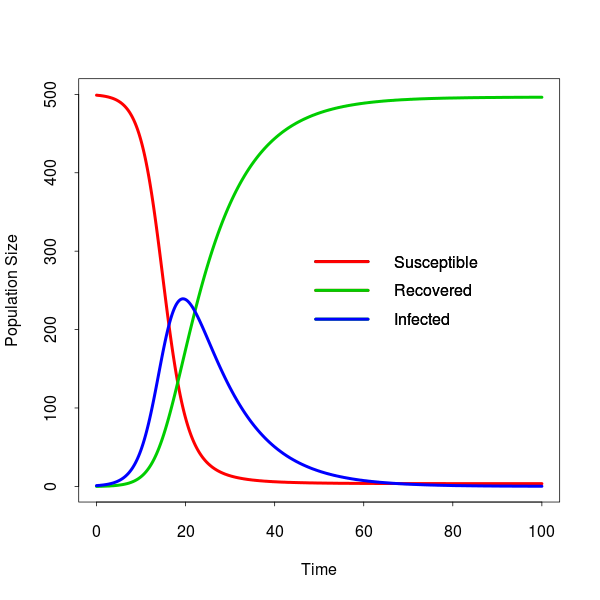
\includegraphics[width=120mm]{Rplot.png}
\caption{Generic example of the classic SIR model demonstrating the change in population size for each compartment as the epidemic unfolds}
\label{sir}
\end{figure}

\begin{equation*}
N = S(t) + I(t) + R(t)
\end{equation*}

The way in which individuals individuals move between these compartments are described by the following set of ODEs:
\begin{equation*}
	\begin{split}
	&\frac{dS}{dt} = -\beta IS, \\
	&\frac{dI}{dt} = \beta IS - \gamma I, \\
	&\frac{dR}{dt} = \gamma I
	\end{split}
\end{equation*}

The dynamics of these ODEs are influenced by two key parameters: the contact rate, $\beta$, and the recovery rate, $\gamma$. $\beta$ describes the probability of an infected person coming into contact with any susceptible person per unit time, whereas $\gamma$ describes the rate at which an individual recovers from the disease. When $\beta$ is large, the contact rate between individuals is high, and the disease spreads rapidly. Similarly, when $\gamma$ is large, then individuals recover rapidly and move to the recovered compartment quickly. Note that these parameters make global assumptions about the population, in that all individuals have an equal chance of interacting, and all individuals recover at the same rate. Infected individuals therefore come into contact with $\beta$$N$ individuals per unit time. Only susceptible individuals may become infected, and the number of new infections per unit time is therefore $\beta$$N(S/N)$, resulting in a new infection rate of $\beta$$N(S/N)I = $$\beta$$SI$. Finally, as individuals recover with rate $\gamma$, they are removed from the infected compartment and enter the recovered department with rate $\gamma I$.

Considering these parameters allow for useful insights into the dynamics of a given disease: a disease with a high $\beta$ and lower $\gamma$ will obviously spread more than one with a lower contact rate and higher recovery rate. With this in mind, we can make the intuitive leap to conclude that an infection will either: spread as an epidemic when each individual is causing more than one secondary infection; remain endemic in a population when each individual causes exactly one further infection before recovering; will die out when each individual causes less than one secondary infection before recovering. This idea is formalised by the concept of a \emph{basic reproductive number}, $R_0$ (not to be confused with $R(0)$, which denotes the initial size of the recovered population!). $R_0$ denotes the number of secondary infections caused by a single infected individual when introduced into an initial susceptible population, $S(0)$. As this infected individual will come into contact with $\beta N$ individuals per unit time over a period of $1/$$\gamma$ (the mean infectious period), the reproductive number will be given as the number of secondary infections per unit time multiplied by the amount of time that an individual can infect others:\cite{anderson, diekmann}

\begin{equation*}
R_0 = (\beta N)/\gamma
\end{equation*}

$R_0$ describes the number of secondary infections resulting from one individual in a completely susceptible population; however, this rate will obviously decrease as the proportion of susceptible individuals in the population decreases. Rather than considering the initial reproductive number, it is often more useful to consider the effective reproduction number, $R_n$ . In simplest terms, $R_n = R_0 \times s$, where $s$ is the proportion of the population that is susceptible ($S(t)/N$).

As an aside, it should be noted that calculating $R_0$ is a crucial stage in understanding how a disease will spread. A high $R_0$ (eg. malaria) means that the disease will spread rapidly, with each individual causing a high number of secondary infections, whereas a low $R0$ (eg. monkeypox) means that a disease will spread slowly.\cite{vynnycky} As discussed above, an $R_0$ greater than 1 is necessary for an epidemic to take hold. Even at an early stage of an epidemic, $R_0$ can be estimated based on the growth rate of an epidemic, as was the case during the 2003 SARS virus.\cite{sars} Therefore, decreasing the proportion of sucseptible individuals below a certain level (ie. through vaccination) will result in an effective reproduction number of less than 1, preventing the epidemic from taking hold. This critical threshold is defined as the \emph{herd immunity threshold}, and provides a crude but often effective target for immunization programmes:\cite{cockman}

\begin{equation*}
HIT = 1 - \frac{1}{R_0} = \frac{R_0 -1}{R_0}
\end{equation*}

The model shown above describes three compartments, however there are a number of extensions to this model where different compartments and interactions might be appropriate. For example, an "exposed" compartment might be added which encompasses individuals that have been exposed to the disease, but are not yet infectious. Such a model is known as the SEIR model. As well as additional compartments, the transitions between these compartments might be varied. For example, in cases where immunity is only transient, individuals might be able to re-enter the susceptible compartment following recovery (the SIRS model). Choosing the model structure is dependent on the nature of the disease and population under consideration. For example, using an SIS (infected individuals return to the susceptible state) to model HIV, or an MSIR model (initial maternal-derived immunity) in the case of measles.\cite{vynnycky} 

It should be noted that there are further considerations to take when modelling real epidemics. For example, the inclusion of birth and death rate, seasonal dynamics, stochasticity and age-dependent interactions.\cite{vynnycky} However, the basic principles discussed above are sufficient to begin considering how we might model the spread of other epidemic processes. 

With the solid theoretical basis described above, advanced mathematical and computational models are becoming increasingly central to making public health decisions. One recent application of mathematical models in epidemiology was to describe and predict the dynamics of an epidemic in real time.\cite{kerkhove} A study by Tizzoni et al. used a Monte Carlo Maximum Likelihood (MCML)-based approach on historical data from the 2009 flu pandemic to develop a global stochastic simulation model, referred to as GLEAM, to obtain basic model parameters.\cite{gleam, gleam2} (Note that this project will aim to similar methodologies to fit epidemic models in real time, and a brief overview of maximum-likelihood estimation and least squares estimation is provided in Box 1). Tizzoni et al. used GLEAM to estimate the seasonal transmission ability of the 2009 H1N1 pandemic, generating forecasts for the activity peaks in the northern hemisphere. The robustness of this stochastic forecast was also explored as a function of data completeness by fitting the model using only partial data.\cite{tizzoni} 

Tizzoni et al. showed that the GLEAM model was in good agreement with
the actual 2009 epidemic data, even when only partial data was used
(for example, pre-exposure immunity and adherence to vaccination
campaigns. However, a key feature of the model is that it accounts for
the way in which  populations interact and connect, and it was shown
that model accuracy was reduced considerably when using only a partial
dataset for population mobility. The GLEAM model uses three layers: a
population layer (a grid representing the population of the world); a
mobility layer (using real flight data to represent travel between
cells in the grid); and an epidemic model (consisting of susceptible,
latent, symptomatic infectious able to travel, symptomatic infectious
unable to trabel, asymptomatic infectious and permanently covered
compartments). Indeed, consideration of multiple networks layers in
epidemic modelling is a growing area of consideration for real
infectious diseases, as it alows for the consideration of more
realistic population dynamics.\cite{gefm} \\\\

\newpage
\begin{framed}
{\begin{center}{\bf Box 1}\end{center}}
To fit model parameters in real time, we consider two methods to fit a continuous-time model to a given set of data: least squares and Maximum Likelihood Estimation (MLE).

{\bf Least squares} is the simpler of the two approaches, and assumes that the only source of variability in the data is measurement error (which is distributed symmetrically with a constant variance eg. Gaussian). By estimating the "least squares" for a set of parameters, we aim to find the set of parameters that minimises the sum of the squares of the errors (ie. the difference between an observed value and the fitted value). 

More formally, given a simple data set of $n$ points of the form $(x_i, y_i)$, we aim to minimise the following formula:
\begin{equation*}
S = \sum\limits_{i=1}^n r_{i}^2
\end{equation*}

Where $r_i$ is the residual for each point, given by the difference between the actual value of the dependent variable and the variable fitted by the model: $r_i = y_i - f(x_i, \beta)$

In the context of our SIR model, we aim to find the $\beta$ and $\gamma$ values that provide the best fitting SIR model for a given epidemic dataset (we will use the Nelder-Mead algorithm with \emph{R}).\cite{marily2013}

{\begin{center} 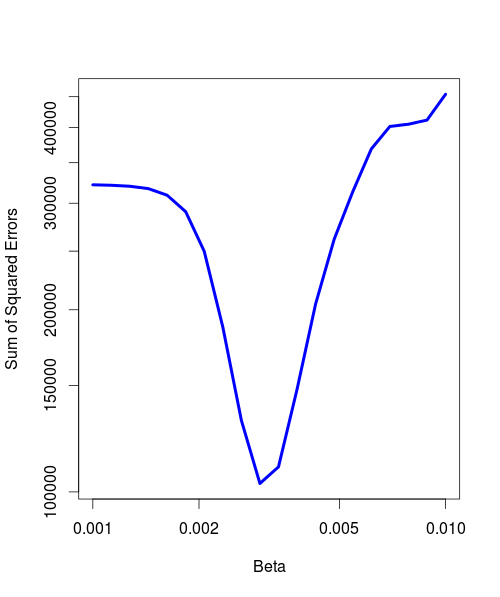
\includegraphics[width=100mm]{sse.png}\end{center}}

Shown above is an example sum of squared errors (SSE) plot demonstrating how a particular value for $\beta$ minimises the SSE to a given dataset at around 0.003. This plot was created using a test flu dataset. Note that this plot assumes a $\gamma$ value of 1, though multiple parameters may be optimised simultaneously using R's \emph{optim} (Nelder-Mead) function.

{\bf Maximum-likelihood estimation} (MLE) is the method of estimating the parameters of a statistical model based on a given hypothesis and a set of data that has occured. This method essentially selects the set of values for the model parameters that maximise the likelihood function:
\begin{equation*}
	\mathcal{L} (\theta | x) = P(x | \theta)
\end{equation*}
In other words, we aim to find the set of parameters that  provide a model fit would be most likely to produce our given data. As above, we aim to find the set of parameters, $\beta$ and $\gamma$ that maximise this likelihood function. Specifically, we calculate the negative log-likelihood of the data given some combination of parameters. Methods using MLE are very common when fitting epidemic models in real time.\cite{white, hall, nishiura}
{\begin{center} 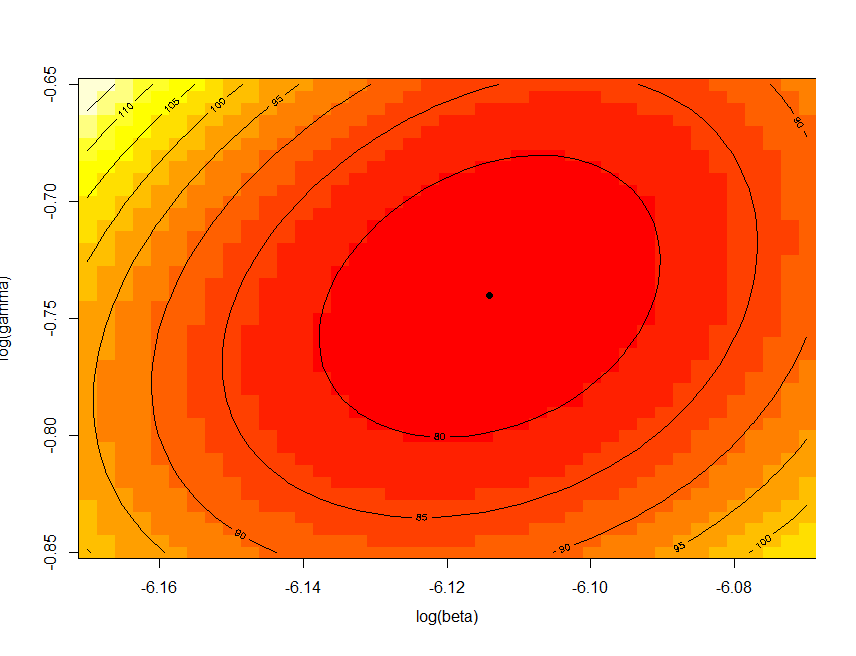
\includegraphics[width=140mm]{logmle.png}\end{center}}
The graph above depicts the two-dimensional parameter space (the likelihood surface) for beta and gamma when fit to a set of epidemic data. Note that we use log values to avoid underflow/overflow.  Each point represents a separate fit to the data, and the height of the surface shows the negative log-likelihood of that parameter combination. In this particular example, we find that a log(beta) value of ~-6.11 and a log(gamma) value of ~-0.74 provide the best fit. We can also show the confidence intervals for each parameter in the form of a likelihood profile, as shown below.

{\begin{center} 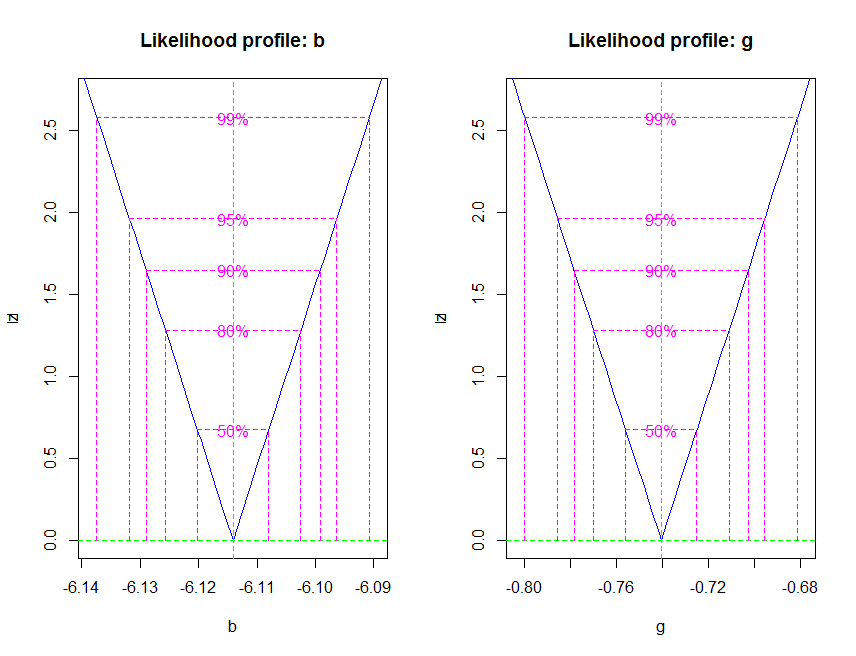
\includegraphics[width=140mm]{mle.png}\end{center}}

\end{framed}

\section{Epidemic Phenomena on the Internet}
A more recent application of epidemic modelling methods is to the spread of information and trends. In particular, the continual development of the internet has opened up a vast area of research into the dynamics of social networks, viral marketing and computer security. It is quite easy to see the analogy between the spread of an online trend to the spread of an infectious disease: individuals have either been exposed to the trend or not; may be actively spreading the trend; or may have lost interest in the trend. The relatively recent surge of interest in online social networks and rapidly rising occurence of viral phenomena has brought with it an interest in understanding and modelling these trends. In this section, we will briefly discuss the history of epidemiology-based analyses of information dissemination and the resulting application of classical epidemiology to online phenomena.

The first application of epidemiology in a social context was made by Goffman and Newill in 1964 who directed attention to the analogy between the spreading of an infectious disease and the dissemination of information.\cite{goffman} This was closely followed by Daley and Kendal, who examined the spreading of rumours using mathematical epidemiology.\cite{goffman} As in Kermack and McKendrick's SIR model, Daley and Kendal used three compartments to describe their population: those individuals that had not heard the rumour, those that were actively spreading the rumour and those that were no longer spreading the rumour. The way in which these compartments interacted was described by parameters indicating those that heard the rumour and those that lost interest or `forgot' the rumour, corresponding to $\beta$ and $\gamma$. Daley and Kendal found that the fit was somewhat limited by the difference in behaviours of a rumour and an infectious disease. Specifically, the way in which individuals "lost interest"  in the rumour was not comparable to recovery from an infectious disease. Although not a perfect fit, Daley and Kendal's study did highlight the potential application of mathematical epidemiology in a social context.

More recently, the ever increasing relevance of the internet to modern day life has resulted in more studies being undertaken to model and predict the spread of trends and information on the internet. Bauckhage et al. present one such study, investigating the application of statistical models in describing the spread of internet memes.\cite{meme} That is, viral catch phrases, images or videos that spread through instant messaging, blogs, forums and social networking sites. Bauckhage et al. use \emph{Google Trends} data as an indicator of search frequency and therefore interest in the internet population. Classiying these as `fads', Bauckhage et al. go on to fit established statistical distributions to over 200 meme related time series compared to a fitted Log-Normal model. Using a multinomial maximum likelihood fit, the authors find that the Weibull, Gompertz and Frechet distributions all provided a better model of general trends for meme related search activity, suggesting that growth dynamics cannot be attributed to chance. The authors conclude that these dynamics can be described as a `hype cycle', encompassing a period of rapid uptake followed by a gradual loss of appeal. Although Bauckhage et al. did not use epidemic modelling, they demonstrated that mathematical modelling could be effectively used to describe online trend dynamics.

\begin{figure}[ht!]
\centering
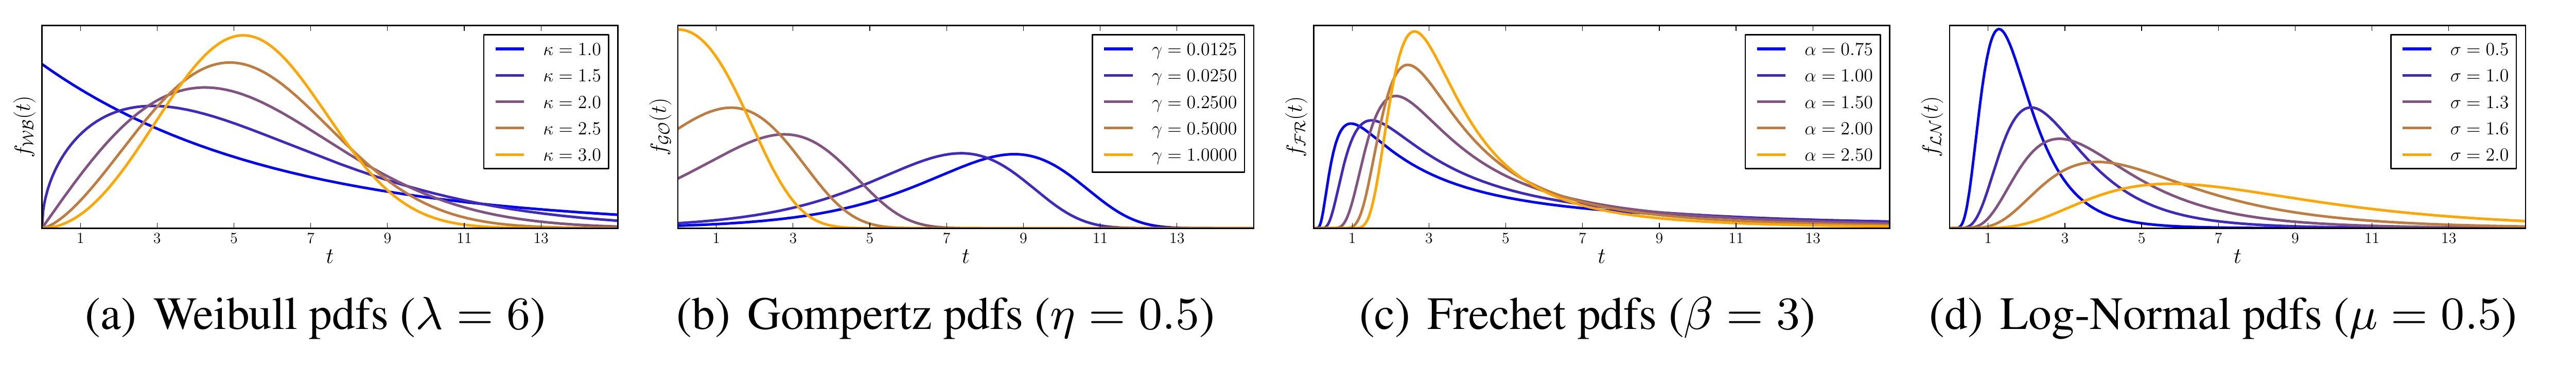
\includegraphics[width=160mm]{statsdist.png}
\caption{Examples of the statistical distributions considered in Bauckhage et al.\cite{meme}}
\label{sir}
\end{figure}

The study by Bauckhage et al. demonstrates the applicability of mathematical modelling to the dynamics of internet memes, however research has also been undertaken to describe the spread of internet `celebrities'. Tweedle and Smith undertook one such study, investigating the usefulness of SIR modelling in describing the spread of popularity of the music artist, Justin Bieber.\cite{bieber} Tweedle and Smith demonstrated that an SIR model could be fit to \emph{Google Trends} search data relatively well. Furthermore, the study investigated how `media effects' might impact epidemic spread (for example, an album release or television appearance). It was found that the inclusion of media effects improved the usefulness of the model in describing the search trend data. Although a fairly `tongue in cheek' study, Tweedle and Smith demonstrated that SIR modelling could be successfully used to describe the spread of online popularity, particularly when additional media effects are considered.

A recent study by Nika et al. showed the potential for epidemiology to explain and predict outbreaks of internet-based information spreading, with the novelty that the size of the initial susceptible population was assumed to be unknown.\cite{marily2013} The aim of this study was to fit SIR and SEIR models to celebrity outbreaks on the internet in real time, improving model fit as the epidemic progresses. Using the Nelder-Mead algorithm with a least-squares-based objective function to fit SIR and SEIR models in real time (see Box 1), Nika et al. were able to demonstrate real time model fitting with unknown initial parameters. The authors validate their approach on synthetic epidemic data, a historical influenza epidemic and BitTorrent and YouTube video views. Both the SIR and SEIR models fit the synthetic and historical data well, and showed good predictive power. However, whilse the models were fit to the internet-based data with some success, the authors acknowledge limitations in their methodology, such as the generation of confidence intervals without due regard for parameter uncertainty. This study demonstrates a promising framework for fitting parameters to data in real time, though highlights the limitations of classic SIR modelling in its basic form.

One recent study using similar methodology that recently received public interest was by Cannarella and Spechler, who investigated the use of SIR modelling in describing public interest in OSNs, namely MySpace and Facebook.\cite{cannarella} Cannarella and Spechler used an adapted SIR model that modified the dynamics of the recovering population such that contact between recovered and infected individuals was required for recovery.  That is, individuals would only stop using the OSN if they came into contact with someone who had already stopped using it. The authors named this adaptation the `irSIR' model. As in the above studies, Cannarella and Spechler used \emph{Google Trends} search data as a proxy for service usage. Similar to Nika et al., the authors used the Nelder-Mean algorithm to find a best fit curve based on sum of squared error, also assuming that all initial parameters, including population size are unknown. The study found that in the case of MySpace, whilst the basic SIR model did not fit particularly well, the modified irSIR model provided a good fit to the adoption and abandonment phases of the OSN. When applied to the ongoing OSN, Facebook, the authors found that Facebook had reached peak popularity in 2012 and was in the early stages of abandonment, predicting that the OSN would reach 20\% of its maximum size by the end of 2014. The authors do concede that there exists an infinite range of possible slower declining solutions. 

Facebook posted a rebuttal to the study, using similar methodology to show that Princeton would cease to exists by 2021 based on Google search results.\cite{facebook} Although not a formal, peer revewed study, Facebook's rebuttal did highlight some shortcomings with the methodology employed by Cannarella and Spechler. Namely the assumption that Google searches were an indicator of usage, and also the flawed assumption that Facebook would not `evolve' to keep users. These studies highlight the importance of making valid assumptions and using appropriate data when attempting to study a rapidly evolving area such as OSNs.

With huge implications for marketing and commercial success, Interest in viral phenomena has become an area of particular interest outside of the academic community. As a result, commercial circles have also taken an interest in attempting to understand the spread of online trends. A review posted by the global strategic insight agency, \emph{Facegroup}, inadvertantly touched upon the application of SIR modelling in explaining the spread of viral videos.\cite{facegroup} The main conclusion that  \emph{Facegroup} came to was that there is no single model of virality. Rather, different types of viral videos could be spread in different ways, proposing `spike' and a `growth' types depending on their spreading pattern. In the `spike' case, videos tend to peak early and drastically drop in views within a week. In the latter case, videos achieve their peak views after a few days and decline slowly, interrupted by secondary peaks of interest. 
\newpage
\begin{figure}[ht!]
\centering
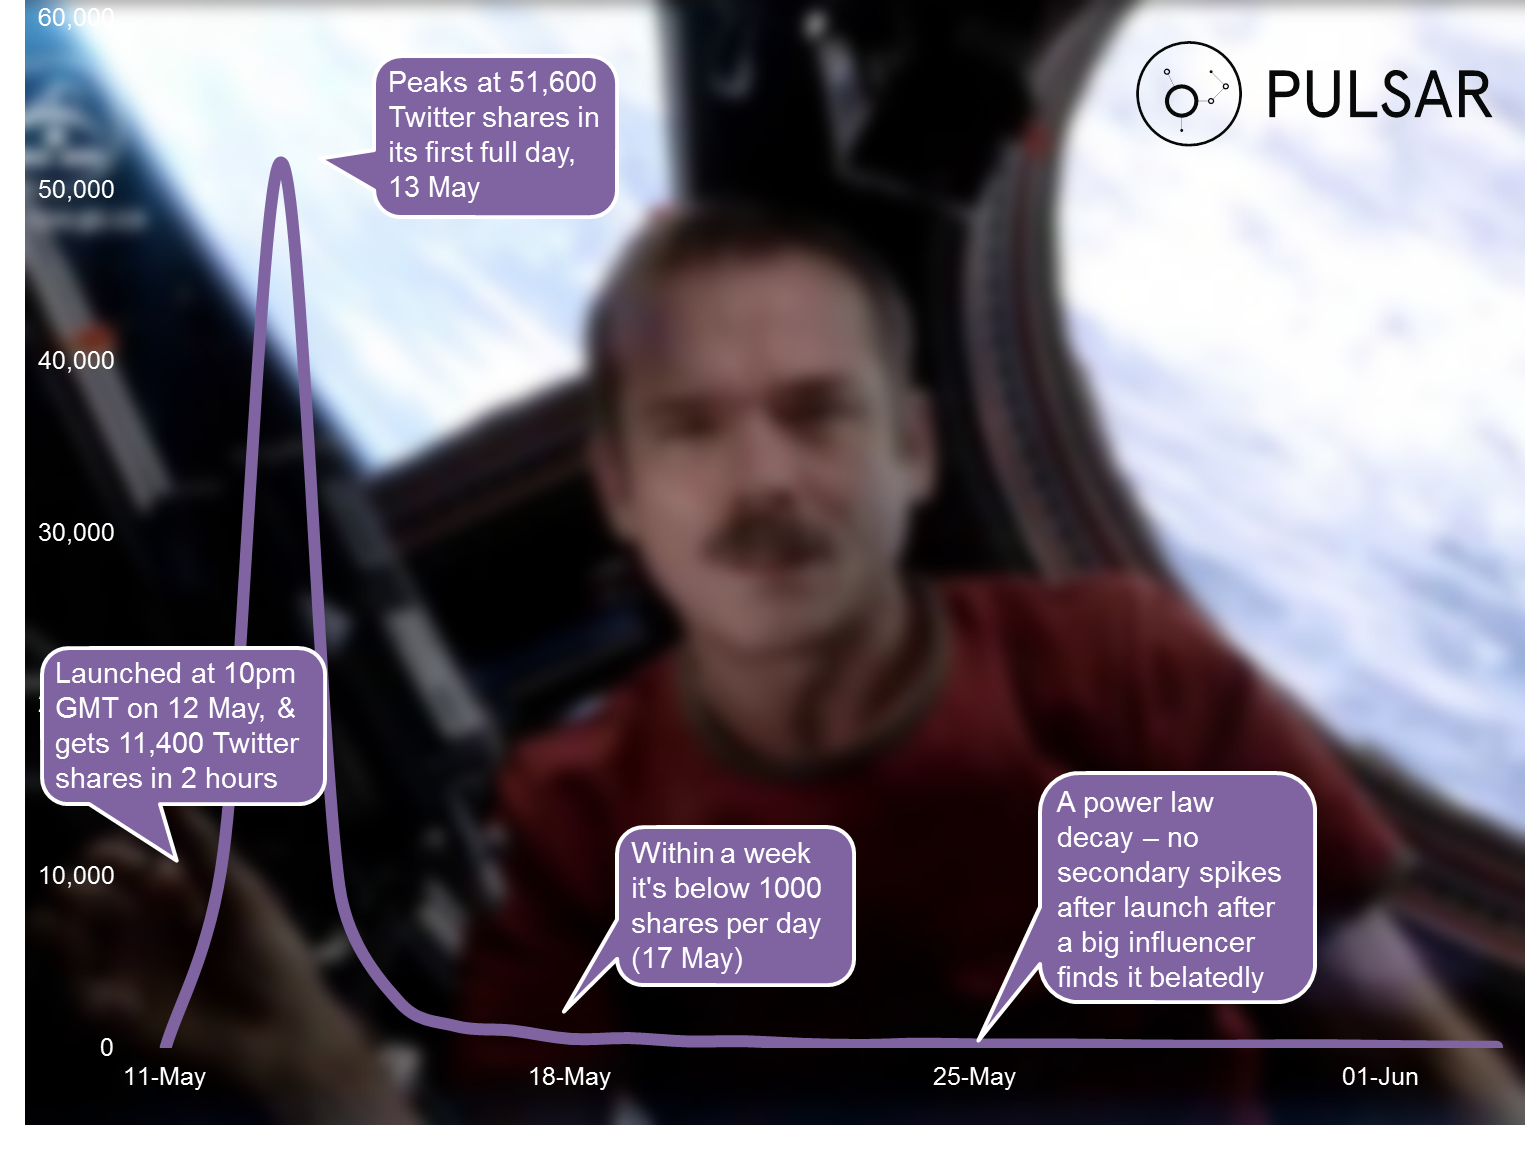
\includegraphics[width=120mm]{hatfield.png}
\caption{Graph \emph{Facegroup} depicting the uptake of the "Commander Hadfield" YouTube video, demonstrating the "growth" model as proposed by \emph{Facegroup}.\cite{facegroup}}
\label{sir}
\end{figure}

\begin{figure}[ht!]
\centering
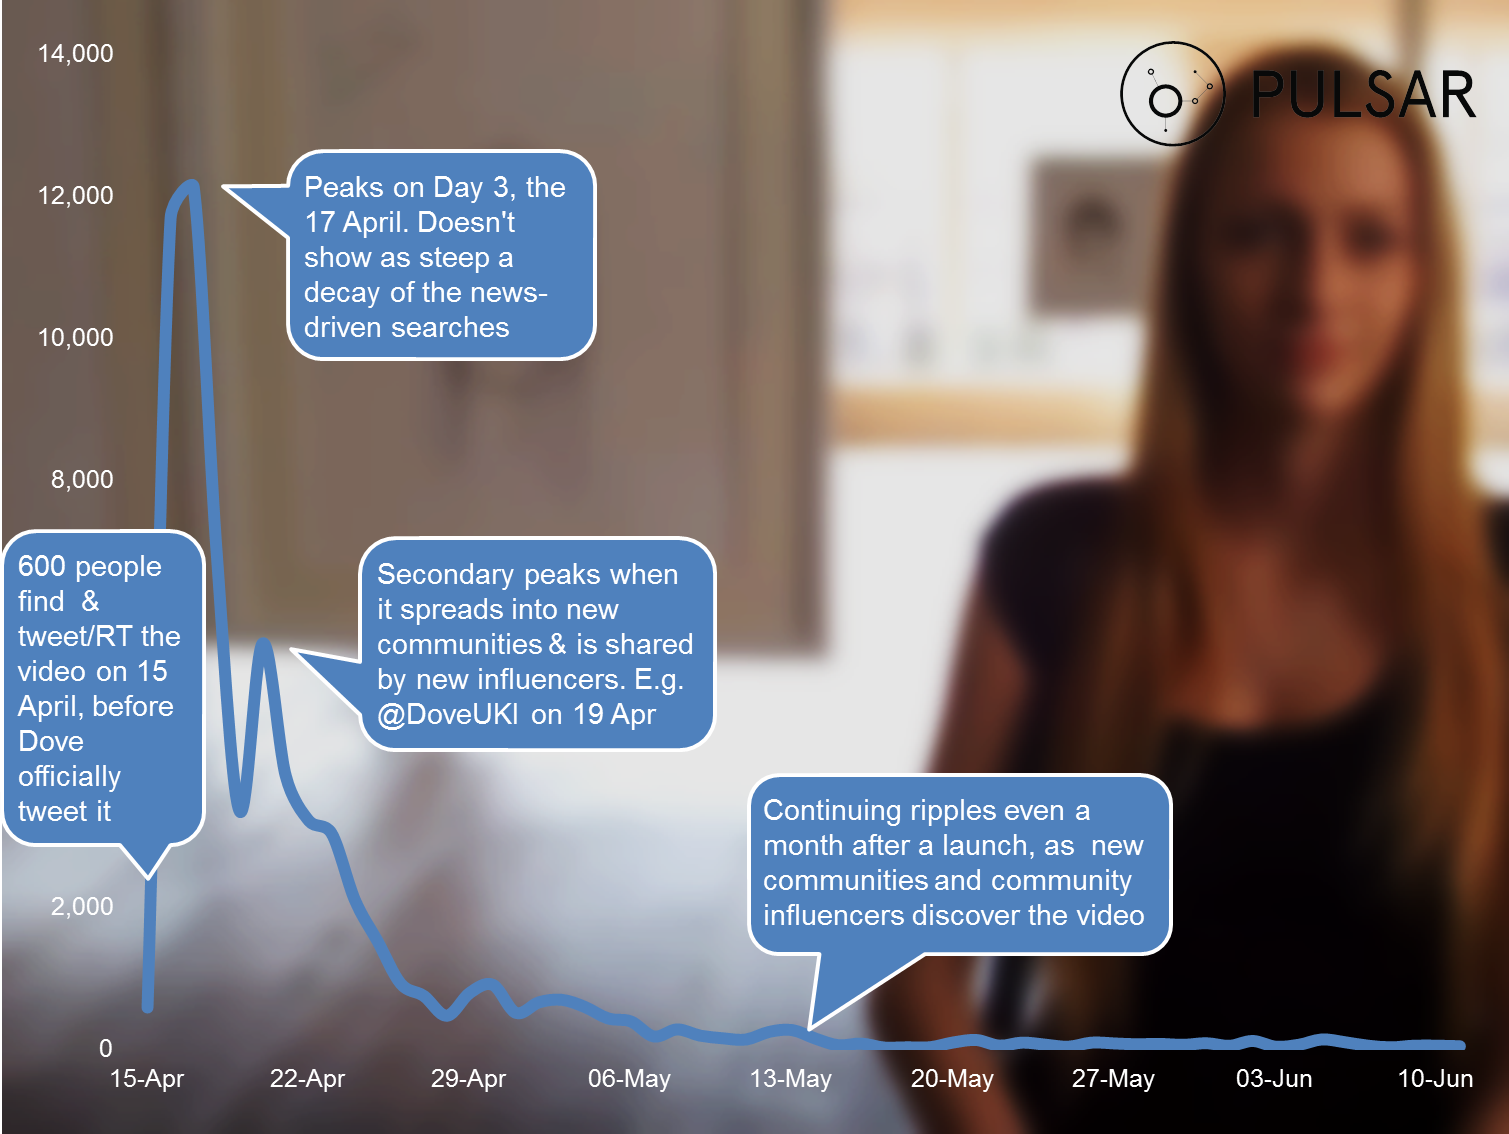
\includegraphics[width=120mm]{facegroup.png}
\caption{Graph from \emph{Facegroup} depicting the uptake of the "Dove Real Beauty Sketches" YouTube video, demonstrating the "spike" model as proposed by \emph{Facegroup}.\cite{facegroup}}
\label{sir}
\end{figure}
\newpage
Returning to an academic setting, Nika et al. recently undertook
another study to improve the fit of their real time fitting framework,
stating that, based on their previous study, a single epidemic is
inadequate to characterise a complex internet-based phenomena. This
may be because internet based trends may be influenced by multiple
underlying spreading mechanisms at different times, similar to the
`media effects' as described by Tweedle and Smith in their analysis of
`Bieber Fever'. Nika et al. took inspiration from Fourier analysis,
proposing that modelling and predicting internet-based phenomena could
be better described by considering multiple compartmental
epidemiological models. That is, an epidemic signal can be broken down
into a number of sub-epidemic models which, when recombined, can be
used as a predictive model (see Figure 1). Nika et al. go on to coin
the term \emph{synthedemic} from the field of syndemics - the idea
that infections can co-occur and interact with each other as well as
environmental factors. 

The term synthedemic is used to describe the co-occurence of a set of
infections, whether they are dependent or not. The aim of the study
was to account for the potential influence of multiple underlying
spreading mechanisms which may begin at different times by breaking an
incoming epidemic signal into component parts, and selecting the model
that best explains each component. Using only a classical SIR model
and exponential decay model as candidates, Nika et al. are able to
adequately characterise the evolution of synthetic data and four
real-world data sets from internet trends (BitTorrent downloads and
daily Youtube views) well. Please refer to Box 2 for a detailed
explanation of the theory used by Nika et al. Using synthetic double
epidemic data, the model by Nika et al. successfully predicts two
overlapping epidemics, predicting the peak of the second, spike
epidemic with a high RSquare value. The model is also fit successfully
to the BitTorrent downloads of two popular songs and a viral YouTube
video; detecting the presence of multiple outbreaks and exponential
decay of interest.
\newpage
\begin{framed}
{\begin{center}{\bf Box 2}\end{center}}
{\bf Methodology}:\\
The modelling procedure begins by considering a small, truncated
dataset of an epidemic outbreak. At each time point, an additional
data point is added until the end of the considered time frame is
reached. This might be a synthetic epidemic dataset, a historical
infectious disease epidemic, or some measure of interest in an online
phenomena (Nika et al. use BitTorrent downloads and daily YouTube
views). Nika et al. propose two candidate models that provide
theoretical analogues to the \emph{growth} and \emph{spike} trends as
proposed by \emph{Facegroup}: an SIR model to represent gradual
growth, and an exponential model to represent a rapid outbreak and
decay of public interest.\cite{facegroup}\\\\

At every time point, the multiple epidemic is optimised by attempting
to minimise the sum of squared error of the model against the data. At
each stage of fitting, the latest residuals are checked at each
additional time point for the presence of an additional epidemic
outbreak. If detected, a new epidemic is temporarily added to the
model from the list of candidate models. If the addition of this model
improves the $R^2$ value, then this additional epidemic is included in
all future model fittings. After the multiple epidemic model has been
optimised, an autoregressive model is fitted to capture the remaining
variability in the data. Finally, thefit of the multiple epidemic AR
model is assessed against benchmarked fitting procedures, such as a
single epidemic model, using a range of statistical tests, including
rSquare comparison.

{\bf Candidate Models}:\\
Let \emph{M} be the class of sub epidemic models under consideration: 

 \begin{equation*} M  = \{f_{1}^{(i)}, f_{2}^{(i)}\} \end{equation*}

Where $f_1^{(i)}$ and $f_2^{(i)}$ are defined as follows:
\begin{enumerate}[label=\Alph{*}.]
	\item $f_1^{(i)}$ denotes the SIR model $f_1^{(i)}(\theta^{(i)}, t)$ with parameter vector $\theta^{(i)} = [I_0^{(i)}, S_0^{(i)}, \beta^{(i)}, \gamma^{(i)}]$
\begin{equation*}
	\begin{split}
	&\frac{dS}{dt} = -\beta IS, \\
	&\frac{dI}{dt} = \beta IS - \gamma I, \\
	&\frac{dR}{dt} = \gamma I
	\end{split}
\end{equation*}
	\item $f_2^{(i)}$ denotes the Exponential decay model $f_2^{(i)}(\theta^{(i)}, t)$ with parameter vector $\theta^{(i)} = [I_0^{(i)}, \gamma^{(i)}]$
\begin{equation*}
	\frac{dI}{dt} = - \gamma I
\end{equation*}
\end{enumerate}
	
Parameter \emph{t} denotes a particular time, where $S_0^{(i)}$ and
$I_0^{(i)}$ denote the initial number of susceptible and infectious
individuals at time \emph{t}, whilst $\beta^{(i)}$ and
$\gamma^{(i)}$denote the infection and recovery rate. Furthermore, the
current number of sub epidemics within the overall model is given by
\emph{k}, where the combined value of the epidemic model at time
\emph{t} is given by the following formula:

\begin{equation*}
	\hat{y}(\theta ,t) = \sum\limits_{i=1}^k f^{(i)}(\theta^{(i)} ,t)
\end{equation*}
\end{framed}

Global mathematical models of epidemic processes provide a useful
insight into infectious disease dynamics; however, they make a number
of potentially unrealistic assumptions. Most notably, SIR models
assume complete mixing of the population. That is, each individual in
the population has an equal chance of coming into contact with every
other individual in the population. Although this assumption may hold
in certain scenarios (it is generally safe to assume that the internet
population observes random mixing), it may not be applicable to many
systems that are affected by local dynamics. Consider the population
of a town comprising of schools, offices and homes. Obviously a
student will mix much more frequently with other students and their
family rather than office workers. In such cases, the approach of SIR
based modelling may not be sufficient to capture the underlying
dynamics of the population. Many researchers have therefore developed
extended models to investigate stochasticity, multiple compartments
representing different subpopulations, branching processes and
chain-binomial models.\cite{computational}

One recent approach of particular relevance to the study of epidemic
phenomena in a social context is that of networked epidemiology: an
approach that encompasses individual behaviour, heterogenous
multiscale networks and the dynamical processes on these
networks. Although this particular project focuses on the application
of classical SIR modelling, it is worth discussing networked
epidemiology in brief to give a complete picture of the field.

\section{Networked Epidemiology and Social Networks} 

We have briefly touched on the idea of networks in epidemiology with
reference to multi-layered epidemic models, however it is worth
discussing the basics behind network considerations.\cite{tizzoni,
  gefm} Networked epidemiology takes its inspiration from graph
theory, using nodes to denote individuals and edges to denote
interactions. 

Let \emph{G(V,E)} denote a contact graph on a population of \emph{V}
individuals, where each edge, \emph{e = (u, v) $\in$ E} denotes those
individuals, \emph{u, v $\in$ V} that come into contact. As in the SIR
model, each node might be in the \emph{ S, I} or \emph{R}
state. However, the key difference is that the infection may only
spread from \emph{u} to \emph{v} along an edge with a probability of
$\beta$(\emph{e, t}) at time instant \emph{t} after \emph{u} has
become infected. Similarly, a node only remains infected for a set
amount of time denoted by $\tau$(\emph{u}). After this time, the node
\emph{u} switches to state $R$. By considering this network model over
a given number of time steps, the dynamics of an epidemic taking place
in a network can be modeled. With this basic idea, it is easy to see
how real world networks structures and data can be used to vastly
improve models of epidemic processes in reality, thereby improving
approaches to vaccination and disease control programmes.\cite{danon}
On the other hand, the reality of transmission networks is not quite
so ideal, with information regarding population connectivity and
interactions being limited. In this section, we will discuss a sample
of studies that build on the concept of local network approaches, and
discuss some approaches that have been taken towards applying these to
online trends.

With the basis for another approach to epidemic modelling, we can
begin to consider general frameworks to describe local dynamical
processes. One such approach is called the graphical discrete
dynamical system (GDDS)\cite{bisset}, which is defined as a tuple
(\emph{G, F, $\pi$)}), where: \emph{G = (V, E)} represents the
underlying contact network;  \emph{F = \{f\textsubscript{v}$|$v $\in$
  V\}} is a set of local functions for each node, \emph{v}, to compute
the state of \emph{v} based on its neighbours; and $\pi$ is a schedule
that specifies the order in which the stages of the nodes are
updated. It is possible to view the configuration space of a GDDS as a
Markov chain, \emph{M}, where each node in \emph{M} is the state
vector of the node states in the GDDS, \emph{G}. For example, in the
SIR model these three states correspond to the susceptible, infectious
and recovered states. 

A conceptually simpler approach to local network modelling is that of
a cellular automata model. Cellular automata models take into
consideration local behaviour and heterogeneity by ascribing each
individual to a particular cell as part of a grid. Individual cells
may have a certain state, such as infected or susceptible, and may
interact with other cells depending on the assumptions made. Turner et
al. provide one such example of this type of model, proposing two
spatial host-pathogen models that are described as equivalent to a
density and frequency dependent global model.\cite{turner} Another
example is provided by Zanette and Risau-Gusman, who investigate the
effect of evolving connections between individuals affects the spread
of an infection. Zanette and Risau-Gusman use an SIS based model where
susceptible agents are able to break their links with infected agents
either temporarily or permanentely, showing that a moderate contact
reconnection frequency is sufficient to suppress
infection.\cite{zanette}  It is possible to stretch the analogy of
human networks to the internet, with towns and cities representing
various internet communities. However, the drastically higher level of
connectivity and transmission speed on the internet does limit the
applicability of these locally driven models.

Global models may provide a more appropriate approach to global
internet trends compared to locally driven models; however, research
into using network based models to describe the dynamics of social
networks has recently shown some success. The aim of such models are
largely to predict future viral trends. One such example is a study by
Altshuler et al., who investigated the use of social diffusion models
in trend prediction in an online social trading
community.\cite{altshuler} Altshuler et al. set out to answer the
following question: given a snapshot of a social network with some
behaviour occurences, what is the probability that these occurences
will result in a viral diffusion and a wide-spread trend? The authors
model the diffusion process using scale-free networks (ie. probability
that \emph{v} has \emph{d} neighbours follows a power law); taking
into account local fluctuations and heterogeneity. From this,
Altshuler et al. develop a theoretical mathematical model to
understand trend diffusion in social networks. However, as the authors
points out, their framework needs to be tested in the field by
conducting an active experiment in which the emergence of a trend is
predicted in real time.

\section{Summary}
Research into the mathematical modelling of epidemic processes is now
an established field, with the majority of work based on the original
SIR model as proposed by Kermack and McKendrick.\cite{kermack}
Extensions of the SIR model take into account additional compartments
and inter-compartment dynamics, such as the inclusion of an `exposed'
group or of births and deaths. By customising model parameters and
structure, public health authorities and researchers can improve their
understanding of the way in which infectious diseases spread. For
example, using an SIS (infected individuals return to the susceptible
state) to model HIV, or an MSIR model (initial maternal-derived
immunity) in the case of measles.\cite{vynnycky} Understanding these
population dynamics in combination with the critical vaccination
threshold, given by the reproductive ratio of the virus, allows for
effective vaccination and control strategies. Particular topics of
note in recent years are the use of multi-layered epididemic models
and the use of maximum-likelihood estimations to predict the spread of
an epidemic in real time. \cite{tizzoni, gefm, white, hall, nishiura}

Although infectious diseases are the focus of mathematical modelling
of epidemic processes, a novel application is in the modelling of
internet-based phenomena and trends. As online social networks and
content sharing site become increasingly popular, the relevance of
understanding the dissemination of information online becomes an
increasingly important area of research both from an academic and
commercial perspective.\cite{cannarella, facebook} Studies in this
area are still at an early stage, though a few recent studies have
shown promising early results. \cite{marily2013, marily2014, bieber}
The study by Nika et al. shows promising results be considering the
presence of multiple, overlapping epidemics to describe one epidemic
phenomena in real time using a least-squares based fit. That is, the
popularity of a single online trend may be described through
considering its underlying sub-epidemic components. Nika et
al. consider two types of sub epidemic model as proposed by the
strategic insight agency, \emph{Facegroup}, and is the first study to
consider multiple overlapping epidemics to explain the spread of
internet trends. 

Although applying epidemic modelling techniques to the spread of
internet trends has shown promising results, there are a number of
limitations and flawed assumptions that must be considered. Firstly,
the analogy between an internet trend and an infectious disease is
limited. Nika et al. point out that whereas normal SIR modelling will
be able to make realistic assumptions or measurements regarding the
size of the initial susceptible population, this is not possible when
considering online trends. This $S_0$ value must therefore be treated
as an additional unknown parameter.\cite{marily2013} Furthermore, the
spreading mechanisms and lifecycle of internet trends are different to
those of infectious diseases. Whereas infectious diseases must be
passed on through physical contact, internet trends can be spread
instantaneously to any other user through a `tweet' or `share'. Trends
such as online videos or memes may also typically experience media
spikes when a video or celebrity is shown on television or highly
frequented web pages. The dangers of making such assumptions can be
observed in the study by Cannarella et al. who attempted to show that
Facebook would be abandoned by 2015, neglecting to consider that
Facebook will continue to `evolve' to keep users.\cite{cannarella,
  facebook} Proxies for interest in internet trends such as
\emph{Google Trends} search results should therefore be used with
caution.

Despite these limitations, promising early results encourage the
pursuit of further research. There are a number of other techniques
and models currently being investigated in infectious disease
modelling that might be applicable to the spread of internet
trends. For example, the use of maximum-likelihood estimations rather
than least squares;\cite{tizzoni} the use of multi-layered epidemic
models that might account for underlying social network structure (for
example, the spread of a viral video on or between social network
sites);\cite{altshuler, tizzoni} and the consideration of alternative
compartmental models or statistical distributions.\cite{meme}

With so many potential routes to follow, this project will focus on furthering the work done by Nika et al. to fit a multiple epidemic model in real time to the spread of online phenomena.

\section{Development Environment}
\subsection{Programming Languages}
There were a number of candidate programming languages, each with
their own strengths and weaknesses. In the end, R and C++ were chosen
for intitial and final implementations. Previous
approaches to epidemic and synthedemic model fitting frameworks use R
due to its readily available ODE solvers, optimisation functions and
graph plotting functionality.\cite{marily2013,marily2014} R therefore
provided an ideal means to implement the single and multiple epidemic
fitting frameworks initially. Once this initial model fitting
framework was implemented, we went on to provide a C++ implementation
with the aim of providing a faster, more transparent `from scratch'
fitting methodology.

At the start of the project, it was desirable to begin exploring and
understanding the theory behind epidemic modelling and otpimised model
fitting. As such, the first development consideration was to decide on
a language that was well adapted for easy implementations with a large
number of available packages and functions. R and Matlab were
candidates for this initial approach. Whilst Matlab has an arguably
better programming environment with better documentation, R has
already been shown to be effective in epidemic model fitting. The R
community provides a number of statistical analysis tools and is suited to dealing with non-typed data
sets, making it an ideal choice. These packages can easily be obtained
via the Comprehensive R Archive Network (CRAN).

The nature of parameter optimisation means that fitting a large number
of parameters simultaneously can be extremely slow, and an approach to
providing a faster implementation was to reimplement the model fitting
procedure in C++. C++ has been shown to be considerably faster than
both R and Matlab when solving stochastic neoclassical growth models,
suggesting that an efficient C++ implementation might provide a much
faster fitting framework than an R counterpart.\cite{languagespeed}
However, the trade off with run time speed is the fact that coding the
same algorithms and functions in C++ is very time consuming. Whilst
there are R packages readily available that allow parameter fit optimisation,
maximum likelihood estimations and graph plotting in only a few lines
of code, the equivalent functionality in C++ had to be implemented
from scratch. A significant challenge of this project was therefore to
find, adapt or create source code for the essential functions of the
model fitting framework. For graph plotting, a Gnuplot iostream was called from C++
code. 

Python and Java were also considered as potential languages for a
faster implementation. However, the relatively lower speed of Python and
unfamiliarity with Java meant that C++ remained the ideal choice.

It should be noted that whilst C++ provides an ideal way of speeding
up computational bottlenecks in the model fitting procedure (namely
the optimisation step), it it may still be desirable to call R
functions from within the C++ program. For example, the generation of
a likelihood profile. This can be achieved using the
Rcpp library if needed. Furthermore, the quick generation of synthetic
data with which to evaluate and develop the fitting framework is
clearly not a limiting factor. R therefore remained the ideal language
for syynthetic data generation using \emph{GillespieSSA} package,
exporting the data as a .csv file to be imported in the C++ implementation. 


% body of thesis comes here
\chapter{Single Epidemic Fitting}
\label{ch:single}

In this section we explore the theory and implementation behind a
model fitting framework for single SIR models with unknown
parameters. To provide a simulation of real time model fitting, we
iteratively fit a new, independently optimised model at each data point. Firstly, a
least-squares fitting procedure is implemented in R for a single SIR
epidemic where beta and gamma are assumed to be entirely
unknown. We then extend the implementation to include the number of
initial susceptible individuals, S0; the start time
of the epidemic, t0; and the initial number of infected individuals, I0. This also raises
the issue of epidemic outbreak detection and candidate model selection, which we
will revisit in section SECTIONNNN!. We go on to use a maximum
likelihood based approach which allows for the generation of
confidence intervals. Finally, we reimplement the above approaches in
C++ to provide a much faster fitting framework.

\section{Epidemic Data}
The data that we wish to characterise is the change in number of
infected individuals over time. In this context, the term `infected individuals' may be
defined as individuals infected with a disease, or individuals that
have viewed a particular \emph{YouTube} video or `liked' a particular
\emph{Facebook} post. Examples of this type of data are shown in
Figure~\ref{figure:examples}. \emph{R} is ideally suited for the easy management and
manipulation of data through the use of the `data frame' type. In C++,
we import data as .csv files and carry out all manipulation and use
using vectors.


\begin{center}
\begin{figure}[ht!]

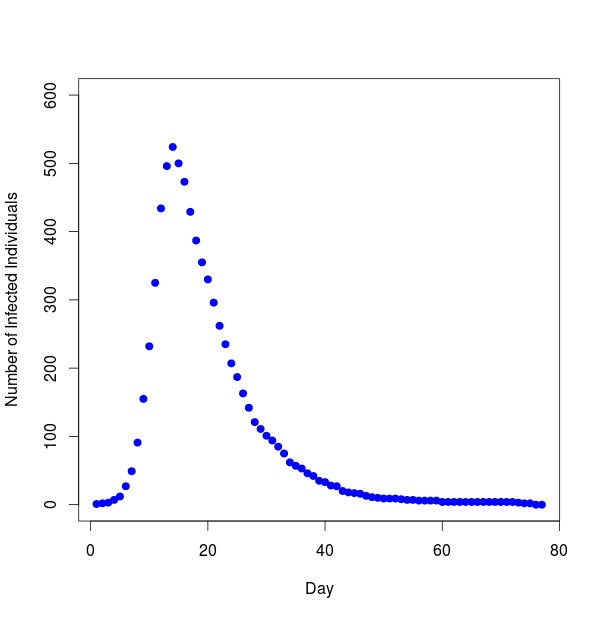
\includegraphics[width=15cm]{simplesir.png}
\caption{Example synthetic epidemic data generated using the
  \emph{GillespieSSA} algorithm in \emph{R}. In this model: $beta =
  0.0015, gamma = 0.1, S0 = 800, I0 = 1$.}
\label{figure:examples}
\end{figure}  
\end{center}

We use the results of solving ODEs with known parameters and
independent runs of the \emph{GillespieSSA} algorithm to test the
framework's ability to find the true model
parameters. \emph{GillespieSSA} provides an easy to use, extensible
means of generating simulated trajectories of finite population
continuous-time models. Algorithm 1 shows a basic implementation of the
SIR model in R using \emph{GillespieSSA} for generation of synthetic data.

\begin{algorithm}
  \captionof{figure}{Implementation of the SIR model using the GillespieSSA package}
  \begin{algorithmic}
    \Function{gillespie.ssa.sir}{$params, I0, time, i$}
    \State \emph{\# Define parameters}
    \State parms $\gets$ c(beta=params[1],gamma=params[2])
    \State
    \State \emph{\# Define system}
    \State x0 $\gets$ c(S=params[3], I=I0, R=0) \Comment{Initial state vector}
    \State nu $\gets$ matrix(c(-1,0,1,-1,0,1),nrow=3,byrow=T)
    \Comment{State-change matrix}
    \State a  $\gets$ c("beta*S*I", "gamma*I")  \Comment{Propensity vector}
    \State tf $\gets$ time \Comment{Final time}
    \State
    \State \emph{\# Run the simulations}
    \State nf $\gets$ layout(matrix(c(1,2,3,4),ncol=2,byrow=T))
    \State
    \State \emph{\# Direct method}
    \State set.seed(i)
    \State out $\gets$ ssa(x0,a,nu,parms,tf,method="ETL",tau=1,
    simName,verbose=FALSE)
    \State return out.data
\EndFunction
\label{algorithm:gillespie}      
 
\end{algorithmic}
\end{algorithm}


\section{Solving Candidate Models}
As we aim to find a model that best describes our data, the next
consideration is the generation of model data that might fit our
epidemic data. With a candidate set of model equations in mind,
namely the \emph{SIR} model, and a set of candidate parameters (beta,
gamma and S0), we solve the model ODEs to generate a series of
discreate data. We can then assess how well this chosen model fits the
epidemic data.

When implementing the model fitting
framework in \emph{R}, we utilise the \emph{ode} function from the
\emph{deSolve} package to return sub-population values calculated from a
given set of parameters, a set of ODEs and a desired time frame. A
simple \emph{R} implementation of the \emph{SIR} is shown in
Figure~\ref{fig:sirR}. In the C++ implementation, an ODE solving
framework is written from scratch.

\begin{algorithm}
\label{fig:sirR}
\captionof{figure}{Implementation of the Kermack-McKendrick SIR model}
\begin{algorithmic}
  \Function{closed.sir.model}{$time, data, parameters$}
  \State S $\gets$ data[1]
  \State I $\gets$ data[2]
  \State R $\gets$ data[3]
  \State
  \State beta $\gets$ parameters[1]
  \State gamma $\gets$ parameters[2]
  \State
  \State dS $\gets$ -beta*S*I
  \State dI $\gets$ beta*S*I - gamma*I
  \State dR $\gets$ gamma*I
  \State
  \State list(c(dS,dI,dR))
  \EndFunction
\end{algorithmic}
\end{algorithm}
  
  
With a model solving framework and a set of data that we wish to fit,
one can begin to visualise how the model fitting process might take
place. Even with completely unknown parameters, candidate models can
be generated by choosing parameters that might fit the
data. Figure~\ref{fig:sircurves} depicts how using various model
parameters results in different
shaped curves. 

\begin{center}
\begin{figure}[ht!]

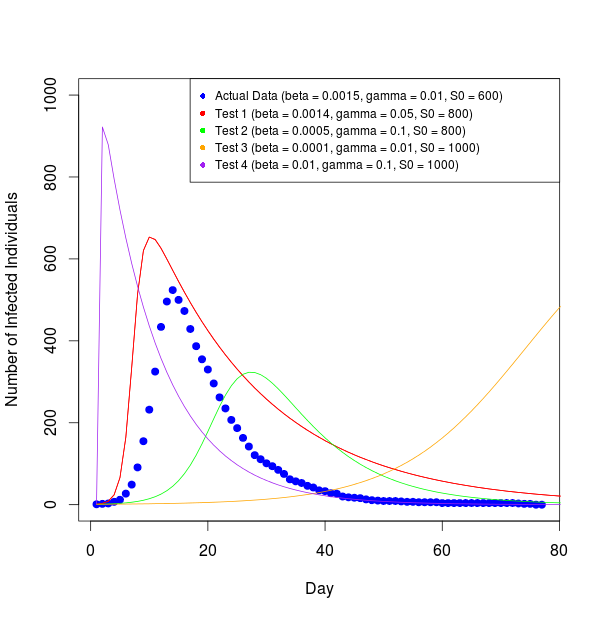
\includegraphics[width=15cm]{Rplot01.png}
\caption{Graph demonstrating various levels of model fit}
\label{fig:sircurves}
\end{figure}  
\end{center}

As a theoretical aside, it should be highlighted that the
\emph{ode} function uses the LSODA integration method by default,
based on FORTRAN code. The benefit of the LSODA method is that is
automatically switches between stiff and non-stiff systems, and is
very robust. However, in our C++ implementation, we provide a `from
scratch' ODE solver using the Runge-Kutta method in an attempt to
speed up the model fitting process. A theoretical introduction to ODE
solving is provided in Box 4.  

\newpage
\begin{framed}
{\begin{center}{\bf Box 4: Solving Ordinary Differential Equations}\end{center}}

The epidemic models take the form of ordinary differential
equations (ODEs), wherein the dynamics of the population are described by the
transition of individuals between different compartments. In the case
of the the \emph{SIR} model, individuals transition from susceptible,
to infected and finally to recovered. As discussed in Box 1, the rate
of transition between these states depends on the model parameters
(namely beta and gamma), as well as the number of individuals
currently in each compartment. 

For the purpose of model fitting, it is necessary to calculate the
number of individuals in each compartment at each time point. This
requires the set of ODEs to be solved. Given a set of parameters and
initial compartment sizes, we wish to find the number of individuals
over the course of the epidemic at each time point. For a simple
differential equation, it is possible to find the closed form
solutions. Given a function, \emph{g}, we wish to find the solution
such that:

\begin{equation}
\begin{split}
  &Y'(t) = g(t)\\
  &Y(t) = \int g(s)ds+c
\end{split}
\end{equation}

where \emph{c} is an arbitrary constant, and the value of Y(t) can be
obtained at a given time point: \begin{equation} Y(t_0) = Y_0 \end{equation}

In the case of
first-order differential equations (as is our case), we take the above
equation as the initial value condition and are presented
with an initial value problem of the form:\cite{atkinson} 

\begin{equation}
\begin{split}
  &y'(t) = f(t,y(t)),\\
  &y(t_0) = y0
 \end{split}
 \end{equation}

It is often impractical to derive analytical solutions to
differential equations. In the case of models in epidemiology, the
first-order different equations are often
non-integrable.\cite{shabbir} Considerable work has been undertaken to attempt to solve
\emph{SIR} models analytically using Lie analysis and homotopy
analysis.\cite{nucci, khan} Such approaches are difficult to implement
and are not fit for the purpose quickly solving ODEs in a
generalisable way. We therefore turn to numerical
analysis.

Numerical methods are used to find numerical approximations to the
solutions of ODEs rather than solving them analytically. For the
purpose of obtaining population values that can be used in model fit
assessment, such numeric approximations are sufficient. The simplest
numerical method for solving the initial value problem is \emph
{Euler's method}, which involves finding an approximate nearby point
on the curve by moving along a line tangent. Euler's method forms
the basis for a highly popular group of
methods for solving initial value problems known as Runge-Kutta
methods, which are relatively easy to implement. 

The most basic member of the Runge-Kutta methods is simply known as
the ``classical Runge-Kutta method'', and is the method that we chose
to implement in C++. Given the above initial value problem and an
initial condition, we can attempt to find later values of y(t) with
the following definitions:

\begin{equation}
\begin{split}
  &y_{n+1} = y_n + \frac{h}{6}(k_1 + 2k_2 + 2k_3 + k_4)\\
  &t_{n+1} = t_n + h
 \end{split}
\end{equation}
for \emph{n} = 0, 1, 2, 3..., using
\begin{equation}
\begin{split}
  &k_1 = f(t_n,y_n),\\
  &k_2 = f(t_n + \frac{h}{2},y_n+ \frac{h}{2}k_1),\\
  &k_3 = f(t_n + \frac{h}{2},y_n+ \frac{h}{2}k_1),\\
  &k_4 = f(t_n+h,y_n+hk_3)
\end{split}
\end{equation}

Note that $y_{n+1}$ is the Runge-Kutta approximation of $y(t_{n+1})$,
where $y_{n+1}$ is determined by the weighted average of four
increments of $y_n$ at interval size, \emph{h}, with the estimated
slope specified by the right hand side of the differential
equations. Note that greater weighting is given to the increments at
the midpoint of the chosen interval.
\end{framed}

\section{Parameter Optimisation}
We now have now clearly identified our problem and the
means by which we can attempt to solve it. That is, can we find a set
of ODE parameters that generate a model that accurately fits our epidemic
data. Given an initial set of test parameters, we attempt to optimise
these parameters to best fit our data using an optimisation algorithm
alongside an objective function measuring model fit.

\subsection{Initial Test Parameters}
In classical epidemiology, it is often possible to obtain estimates of
many important model parameters based on disease biology and
population dynamics. For example, the initial susceptible population
of an isolated influenza outbreak might be estimated as the school-aged
population of a country. Similarly, the infection and recovery rates of a
new strain of virus might be estimated based on phylogenetic relationships
to previous viruses of known parameters.\cite{volz} Another potential method is to measure
transmission rates in experimental populations, as demonstrated by
Bouma et al., who estimated the transmission parameters of the H5N1
avian influenza virus using a small number of birds in an experimental
tranmission study.\cite{bouma} However, it is easy to imagine
situations where parameter estimation might be infeasible. Estimating
the susceptible population size for a viral \emph{YouTube} video, for
example, might be difficult. Do we assume that the entire internet
population is at risk of exposure, or will the video be limited to only
certain internet communities? Such a scenario is not unimaginable for
infectious diseases. Should a new, uncharacterised disease arise in
only an unknown demographic, the task of estimating model parameters
becomes very difficult.

In scenarios where parameter estimation is infeasible, we aim to find
the true model parameters without making any assumptions as to where
they might lie other than within a realistic range. In the presented
model fitting framework, we begin the parameter optimisation procedure
with random parameter values taken from a realistic range with
reasonable limitations imposed. For example, we seed the optimisation
procedure with a random beta value between 0.0001 and 0.01. It is also
important to ensure that a number of realistic conditions are adhered
to:

\begin{enumerate}
  \item The basic reproductive ratio must be sufficient to allow an
    epidemic to take off, $R0 > 1$. For this to be adhered to, gamma
    must be greater than beta.
  \item The initial number of susceptible individuals, $S_0$ must be
    positive and within a reasonable range. Seeding with an
    very high or low values might prevent the optimisation
    procedure from converging on an optimal solution.
  \item The initial number of infected individuals, $I_0$, must be
    greater than 0. Whilst $I_0$ does not necessarily need to be bound
   from above by $S_0$, it is generally the case that $S_0$ is
   much greater than $I_0$. 
\end{enumerate}

One heuristic for estimating the start value of $I_0$ is to take the
first data point as the initial number of infected
individuals. However, this causes the model to be highly dependent on
the first data point, neglecting to consider that the first data point
might not represent the start of the epidemic. A more reasonable
approach would be to consider $I_0$ as another unknown parameter to be
optimised, or to assume that there is initially only one infected
patient, or `patient zero'. In the case of online phenomena, an $I_0$
of 1 may represent the initial posting of a video or meme. In the case
of infectious disease dynamics, $I_0$ might need to be seeded
higher. For example, multiple infecteds might enter a population
simultaneously on the same flight. We initially make the assumption
that $I_0$ is always 1, and then go on to adapt our
implementation to include $I_0$ as an unknown parameter.


\subsection{The Objective Function}
With a set of model equations, potential model parameters and the
resulting model data at each time point, the next step is to assess
how well the proposed model fits the given data. It is only through
quantifying this measurement that we can then go on to find the best
fitting model parameters. As discussed in section BACKGROUND, the
first assessment of fit that we implement is the least squares
fit. This uses the total squared difference between each model
value and dataset value at each time point. The smaller this `sum of
squared errors' (SSE), the better the model fit. Clearly our aim is to find
the set of parameters that minimises this SSE. A central part of the
model fitting framework is therefore the implementation of this
`objective function' (Figure~\ref{algorithm:objective}). Once the objective function is
defined, the final step in the optimisation procedure is to transform
the model parameters until the SSE is minimised.

\begin{algorithm}
 \captionof{figure}{Least Squares Fitting Objective Function}
\begin{algorithmic}
  
  \State \# Takes a set of parameters and a set of
  epidemic data. The \emph{ode} function then uses the LSODA solver to
  evaluate the \emph{SIR} model. The sum of squared
  errors is then calculated from the generated model and provided data.
  \State
  \Function{sir.sse}{$params, data$}

  \State t $\gets$ data[,1]
  \State cases $\gets$ data[,2]
  \State
  \State beta $\gets$ params[1]
  \State gamma $\gets$ params[2]
  \State
  \State S0 $\gets$ params[3]
  \State I0 $\gets$ 1
  \State R0 $\gets$ 0
  \State
  \State out $\gets$ as.data.frame(ode(y=c(S=S0,I=I0,R=R0),
  times=t,closed.sir.model,parms=c(beta,gamma),
  atol=1e-15,hmax=1/120))
  \State sse $\gets$ sum((out\$I-cases)\^2)
  \EndFunction
 \end{algorithmic}
\label{algorithm:objective}
\end{algorithm}


\subsection{Optimisation Algorithm}
The next step in the model fitting framework is an implementation of
an optimisation procedure to find the set of parameters that minimise
the result of the objective function. In the initial \emph{R}
implementation, this is done by passing the initial seed parameters,
the objective function and the data to the \emph{optim}
function. \emph{Optim} uses the Nelder-Mead algorithm to find the set
of parameters in the parameter space that return the minimum objective
function value. That is, the set of parameters that evaluate to a
model that most closely fits the provided data. Box 4 provides a
theoretical overview of the Nelder-Mead algorithm. 

The \emph{optim} function also provides the option to use other optimisation methods,
including the ``BFGS'' quasi-Newton method, the ``CG'' conjugate
gradients method and the ``L-BFGS-B'' method. However, we settle on the
Nelder-Mead due to its robustness, and in the case of C++, its ease of
implementation. 

Figure~\ref{fig:simple}  illustrates the results of running \emph{optim} on a
\emph{GillespieSSA} generated model with known parameters.

\begin{centering}
\begin{figure}
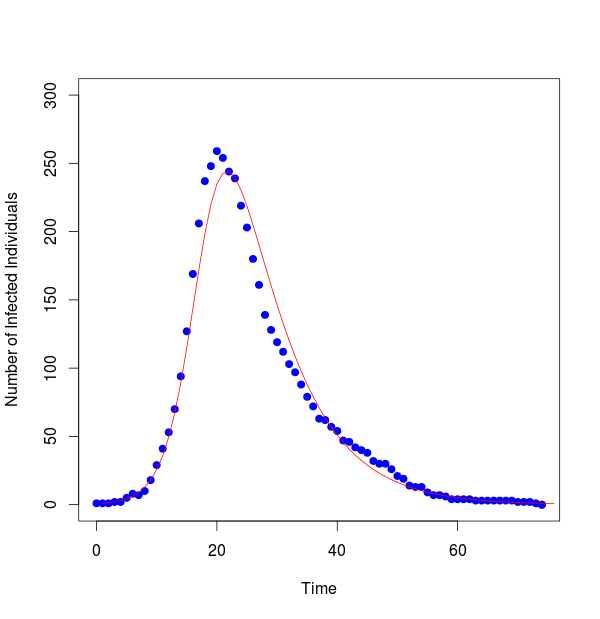
\includegraphics[width=15cm]{simplefit.png}
\caption{The Gillespie algorithm is run with original parameter values of $\beta =
  0.001, \gamma = 0.1, S_0 = 500$. The \emph{optim} function returns
  fitted parameter values of $\beta = 0.0008018066, \gamma = 0.1273486, S_0
  = 618$. This results in a SSE of 5120.06.}
\label{fig:simple}
\end{figure}
\end{centering}



\newpage
\begin{framed}
{\begin{center}{\bf Box 5: The Nelder-Mead Algorithm}\end{center}}
The Nelder-Mead algorithm, or simplex search algorithm, is one of the
best known and commonly used algorithms for multidimensional
unconstrained optimisation without derivatives. The algorithm is
relatively simple to understand and implement, which makes it an ideal
candidate for solving parameter estimation problems. The method
ultimately approximates a local optimum of a problem with $N$
variables when provided with an objective function to be minimised.

Given a nonlinear function, $f : {\mathbb
  R}^n \to {\mathbb R}\ .$, the Nelder-Mead algorithm uses a
simplex-based search method to minimise $f$, where a simplex, $S$
in ${\mathbb R}^n$ is defined as the convex hull of $n + 1$ vertices,
$x_0,...,x_n \in {\mathbb R}^n$. In the case of ${\mathbb R}^2$, the
simplex is a triangle, whereas in the case of ${\mathbb R}^3$, the
simplex is a tetrahedron. In the case of epidemic model fitting, each
vertex of the simplex corresponds to a set of model parameters.

Starting with a set of $n+1$ points (the initial `seed' parameters)
and a corresponding set of function values at the vertices, $f_i :=
f(x_i),$ for $j = 0,...,n$, the Nelder-Mead method performs a sequence
of transformations on the working simplex S with the aim of decreasing
the function values at its vertices. Once the method has satisfied
some minimisation condition, whether it be a number of steps or a
desired minimisation range, the final simplex can be used to return
the optimised parameters.

The Nelder-Mead algorithm follows the following set of
steps:

\begin{enumerate}
\item Construction of the initial working simplex, $S$, around an initial
  point based on initial parameters
\item Repeat the following steps until maximum number of iterations
  reached or minimisation condition satisfied:
  \begin{enumerate}
  \item Calculate the function value for the current working simplex
  \item Check if terminiation criteria met
  \item If not met, transform towards the best vertex of the working simplex to give new
    vertex values with the following sub steps:
    \begin{enumerate}
      \item Determine the order of vertices in terms of function
        values (from best to worst)
        \item Calculate the centroid, $c$ of the side opposite the
          worst vertex
\item Compute a new working simplex from the current simplex using a
  series of transformations
\end{enumerate}
  \end{enumerate}
\item Return the best vertex of the current simplex, S, along with
  its associated function value.
\end{enumerate}

In the transformation step, replacing the worst vertex is achieved by reflection, expansion or contraction with respect to the best
side. Firstly, the worst vertex is replaced with a reflection of the
best vertex. If this point provides an improvement on the current best
value, then the simplex is expanded towards the new point. Otherwise,
the simplex is contracted towards the current best point.If
successful, then the new point replaces the worst vertex of the
working simplex. If not, then the simplex is shrunk towards the best
vertex. A later addition of the algorithm is to shrink the entire
simplex in the event of failed contractions, though this is a rare and
slow step.

\begin{center}
  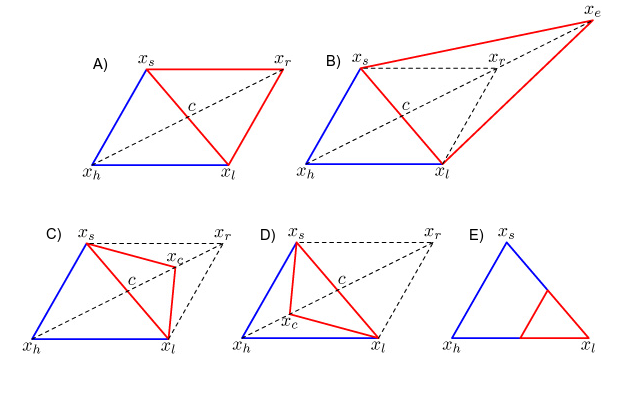
\includegraphics[width=15cm]{nelder.png}
  \captionof{figure}{A) Reflection. B) Exansion. C) Outside
    contraction. D) Inside contraction. E) Shrink transformation}
\end{center}

The Nelder-Mead method is a fast and relatively simple
algorithm for obtaining a good reduction in function value in a
relatively small number of function evaluations. For optimisation
problems where a precise optimum (eg. parameters are subject to noise)
is not necessarily required, the Nelder-Mead method is ideal. However,
it i s possible for the
Nelder-Mead algorithm to undertake an extremely high number of
iterations with little to no function value improvement at a region
far from the actual minimum. A heuristic solution to this problem is
to restart the algorithm at multiple start points and to only allow a
small number of iterations during each run.\cite{nelder,singer}
 
\end{framed}


\subsection{Parameter Transformations and Bounding}
When left unmodified, the Nelder-Mead algorithm will search the parameter
space in the range of $-\infty$ to $+\infty$. However, in the context
of epidemic modelling, it does not make sense to consider negative
parameters. By doing so, we increase the chance of the algorithm
getting stuck in a local minimum and therefore returning infeasible results. We therefore carry out a \emph{log transformation} on each
parameter, only carrying out the reverse \emph{exp} transformation
within the objective function. This constrains the search space to
between $0$ and $+\infty$, ensuring that we do not generate
meaningless parameter vectors. 

Another potential transformation that may be applied is through the
use of the \emph{logistic} function. Originally studied in the context
of population growth, maps the parameter search space from between $0$ and $1$
to between $-\infty$ and $+\infty$. The function is
defined as:
\begin{equation}
logistic(x)=\frac{1}{1+e^{-x}}
\end{equation}
The inverse of the logistic function, the \emph{logit} function, can
therefore be used to map the search space of a parameter, \emph{p},
from between $-\infty$ and $+\infty$ to between $0$ and $1$. The logit
function is defined as:
\begin{equation}
logit(p) = log(\frac{p}{1-p})
\end{equation}
The logit function can be modifed to transform the search space from
between $0$ and $1$ to one between $0$ and $max$ as follows:
\begin{equation}
newLogit(x) = \frac{max}{1+e^{-x}}
\end{equation}
with the inverse defined as:
\begin{equation}
newLogistic(x)=log(\frac{x}{max-x})
\end{equation}

The logic behind this modification can be expanded further to use the
logistic function to provide lower bounds as well as upper bounds. As
$x\rightarrow +\infty$, $logit(x)\rightarrow 1$. Similarly, as
$x\rightarrow-\infty$, $logit(x)\rightarrow 0$. We can therefore modify
the logistic function as follows:
\begin{equation}
f(x) = \frac{x_{max}-x_{min}}{1+e^{-x}} + x_{min}
\end{equation}.

We can see that as $x\rightarrow +\infty$, $f(x)\rightarrow x_{max}$,
and as $x\rightarrow -\infty$, $f(x)\rightarrow x_{min}$. By limiting
the parameter search space to a predetermined range of expected
values, we ensure that the optimisation procedure does not get stuck
in a local minimum far away from the actual parameter values. However,
doing so requires us to make assumptions regarding where the real
parameter values might lie. Whilst a good model fit might be produced
within a provided range of parameter values, this fit might be sub
optimal compared to the model produced from a set of entirely
unexpected parameters. 

An alternative, simple approach to bounding parameter values in the
optimisation procedure is to modify the results returned by the
objective function. As the Nelder Mead algorithm transforms parameter
values with the aim of minimising the objective function, we can
direct the parameter search by ensuring that the objective function
returns high values when venturing into an undesirable parameter
space. For example, we can include a simple check of each parameter
with each call of the objective function; returning a high SSE value
if the parameter is outside our desired range. This method was
implemented initially; however, it appeared to result in the Nelder
Mead algorithm returning nonsense values more frequently as it failed
to identify any local minima. This is due to the fact that the
optimisation surface becomes much less smooth, as each check outside
of the specified bounds results in a sudden spike in function value.  


\section{Evaluating Goodness of Fit}
Although the SSE provides a value which the optimisation process can
aim to minimise, it's magnitude is largely meaningless without
appropriate context. We therefore use the coefficient of
determination, $R^2$, to provide an evaluation of model fit. $R^2$ is
a widely used measure of goodness of fit in statistical modelling, and
provides an ideal means for comparison between different model
fits. $R^2$ provides a measure of what proportion of total variation
in the data is explained by the model. A mathematical definition of
the $R^2$ measure is provided in Box 5.

\newpage
\begin{framed}
{\begin{center}{\bf Box 6}\end{center}}
{\bf The Coefficient of Determiniation}:\\

Consider a data set with observed values $y_i$. We would like to assess how
well a set of predicted values $f_i$ fits our data. Firstly, we
consider the amount of variability in our data set using the sum of
squares:

\begin{equation}
  SS_{tot} = \sum\limits_{i}(y_i - \bar{y})^2
\end{equation}

Where $\bar{y}$ denotes the mean of the observed:

\begin{equation}
  \bar{y} = \frac{1}{n}\sum\limits_{i=1}^n(y_i)
\end{equation}

Next, we calculate the sum of squares of the residuals. That is, the
amount of discrepancy between the data and the predicted values:

\begin{equation}
SS_{res} = \sum\limits_{i}(y_i - f_i)^2
\end{equation}

The final step is then to evaluate the amount of unexplained variance of
the model with the total variance of the data. This gives us the
\emph{coefficient of determination}, $R^2$:

\begin{equation}
  R^2 \equiv 1 - \frac{SS_{res}}{SS_{tot}}
\end{equation}

The resulting value is usually a number between 0 and 1, where 1
suggests that the predicted values explain all of the variance of the
data (a perfect fit), and a value close to 0 implies that it explains
very little of the data
variance (a poor fit). Values of less than 0 are also possible, which indicates
that the mean of the data provides a better model fit than the model.

\end{framed}

\section{Iterative Least Squares Fitting Framework}
\subsection{R Implementation}
Due to the availibility of relevant packages and its suitability for
data manipulation, the initial fitting framework was implemented in
R. The flow of control of the basic implementation is depicted in
Figure~\ref{process}. The framework takes a matrix or data frame of epidemic data
to be fit and begins the optimisation procedure. Random seed
parameters are generated and given to the optimisation function,
\emph{optim}, along with the objective function to be minimised. As
the Nelder-Mead algorithm can converge on sub-optimal solutions due to
the presence of local minima, the optimisation function is restarted
twenty times with different seed parameters. The best fitting set of
parameters are stored and passed to the analysis procedure, which
evaluates the model for the given parameters and calculates the
accompanying R-Square value. Finally, all of the results are passed to
the output procedure for graph plotting and results saving.  

\begin{centering}
\begin{figure}[ht!]
  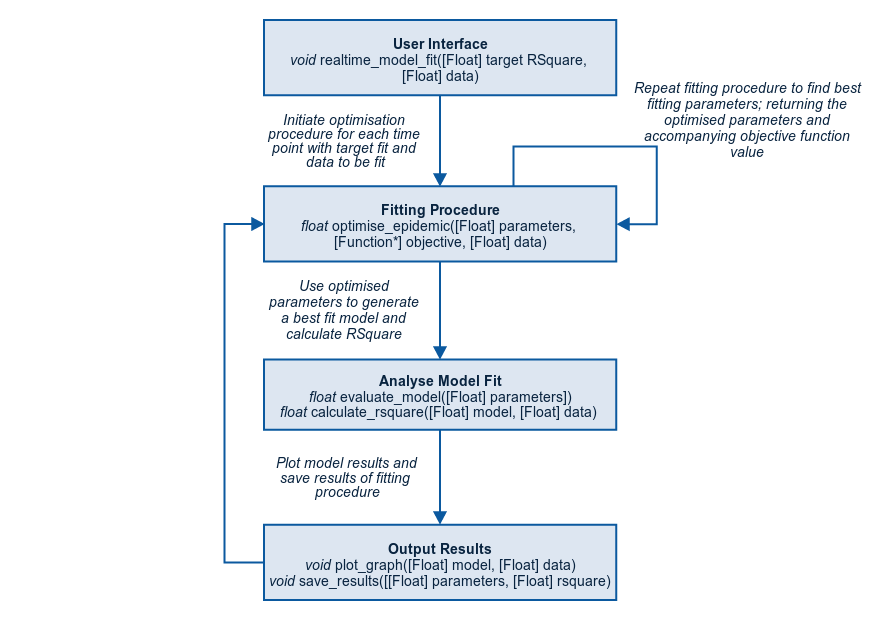
\includegraphics[width=15cm]{images/process.png}
 \caption{Control flow of the basic model fitting framework} 
\label{fig:process}
\end{figure}
\end{centering}

To begin with, the optimisation procedure only considers beta and
gamma to be unknown. The other important model parameters, S0, I0 and
R0 are set to the correct values. We then adapt the framework to also
consider S0 to be a completely unknown parameter. Figure~\ref{fig:sir} shows how the optimisation
procedure unfolds over time. The framework fits the available data
points well early on; however, it does not accurately predict the main
peak until sufficient data has become available. By the 40th data
point, a very high R-Square value is achieved, with parameters that
closely match the ground truth parameters (beta=0.00111, gamma=0.0946,
S0=506). The inclusion of S0 as an additional unknown parameter allows
a closer model fit to be calculated.

\begin{centering}
\begin{figure}[h!]
  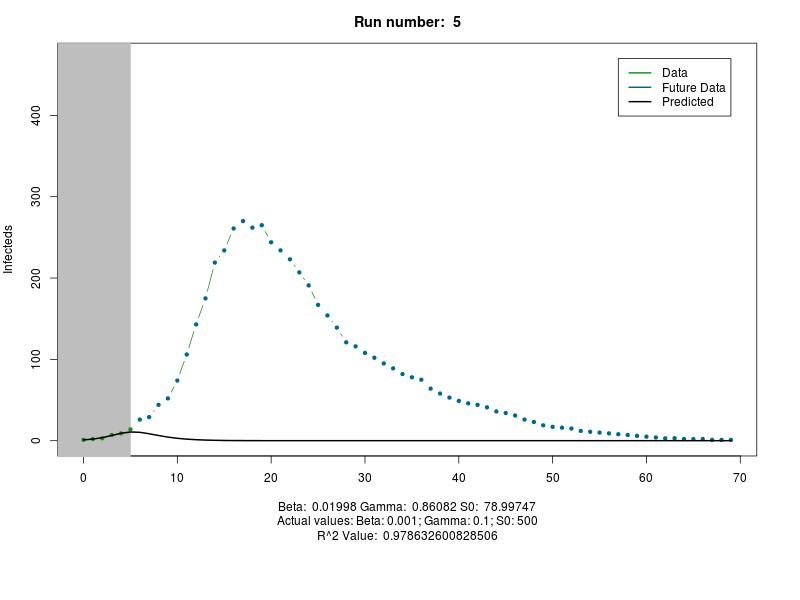
\includegraphics[width=8cm]{images/sirs0_5.jpeg}
  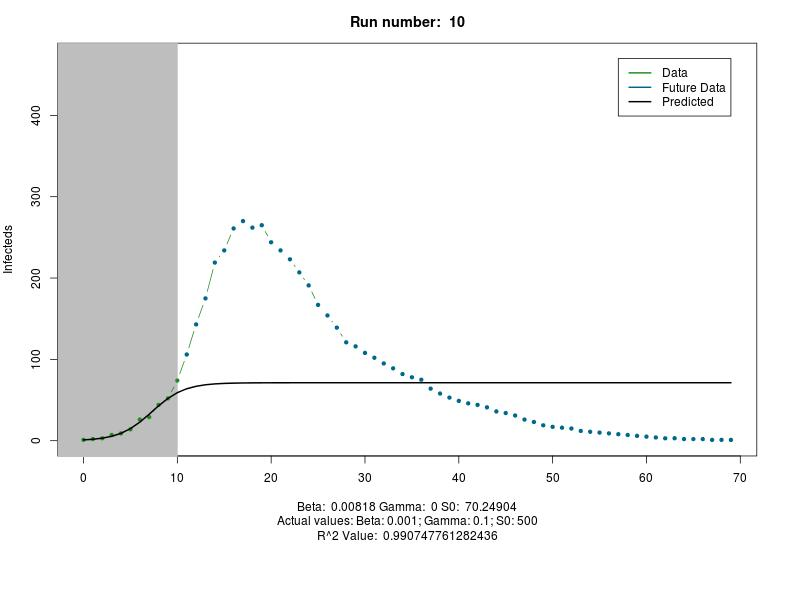
\includegraphics[width=8cm]{images/sirs0_10.jpeg}
  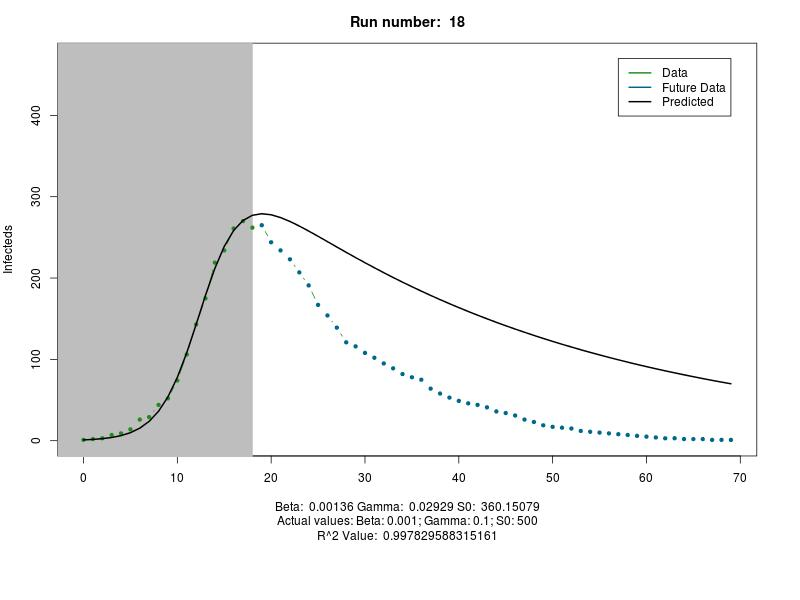
\includegraphics[width=8cm]{images/sirs0_18.jpeg}
  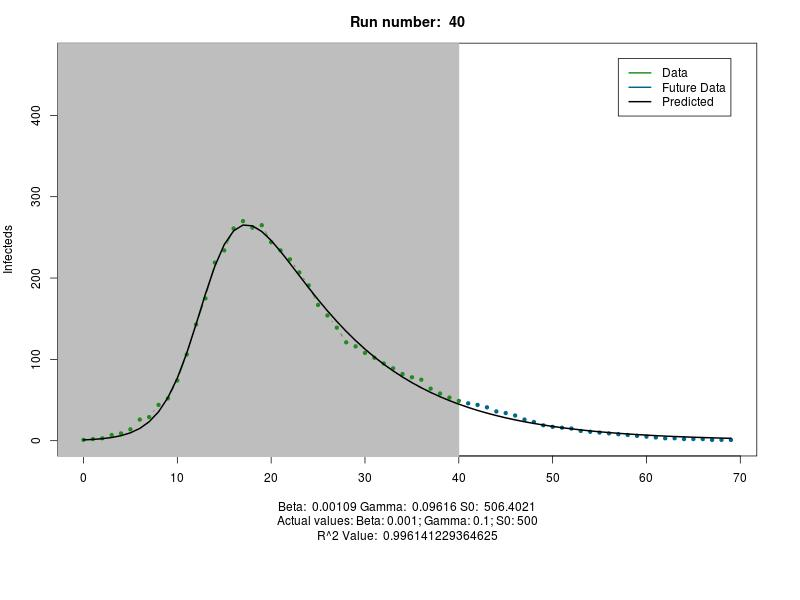
\includegraphics[width=8cm]{images/sirs0_40.jpeg}
\caption{Iterative model fitting over time using least squares
  minimisation.}
\label{fig:sir}
  \end{figure}
\end{centering}

The model fitting procedure can be extended further to include the
number of initial infected individuals, I0. Data from real epidemic
phenomena might not become available until well into the start of the epidemic, and number of initial infected individuals might not immediately
be available. For example, consider a \emph{YouTube} video where views
data are not collected until the video has already become viral. By
including I0 in the optimisation procedure, we
are able to predict the dynamics of the epidemic as soon as it is
detected. Including additional unknown parameters in the
optimisation procedure provides a closer model fit but runs the risk
of increase instability during optimisation as parameter
transformations have a greater impact on the objective
function. Figure~\ref{fig:siri0} shows the run of the optimisation procedure where
beta, gamma, S0 and I0 are all assumed to be unknown. Although the
fits seem comparable to Figure~\ref{fig:sir}, Figure~\ref{fig:siri0wrong} demonstrates how the
goodness of model fit is reduced when our initial assumptions about I0
are incorrect.

\begin{centering}
\begin{figure}
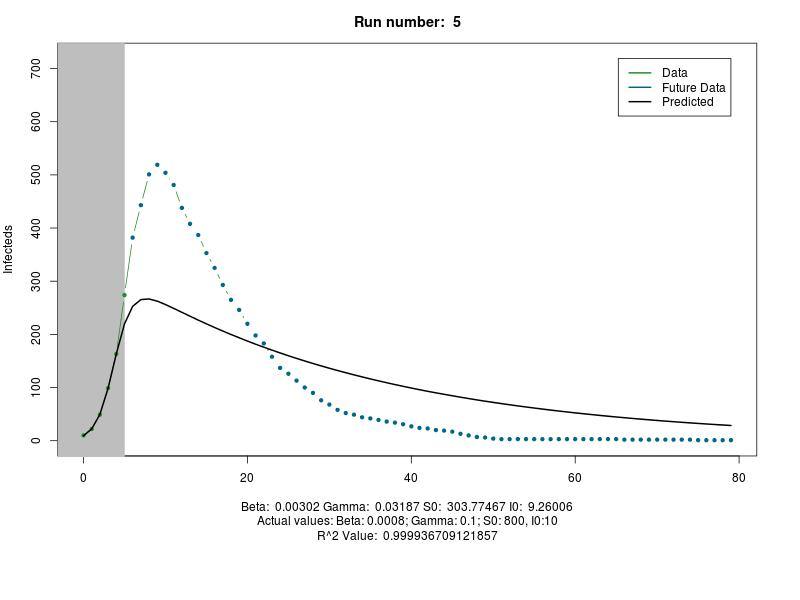
\includegraphics[width=8cm]{images/siri0_5}
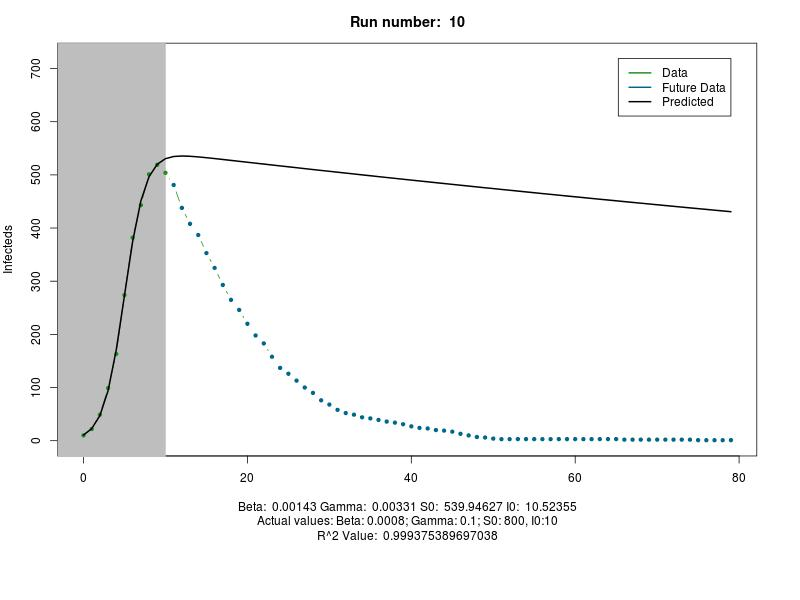
\includegraphics[width=8cm]{images/siri0_10}
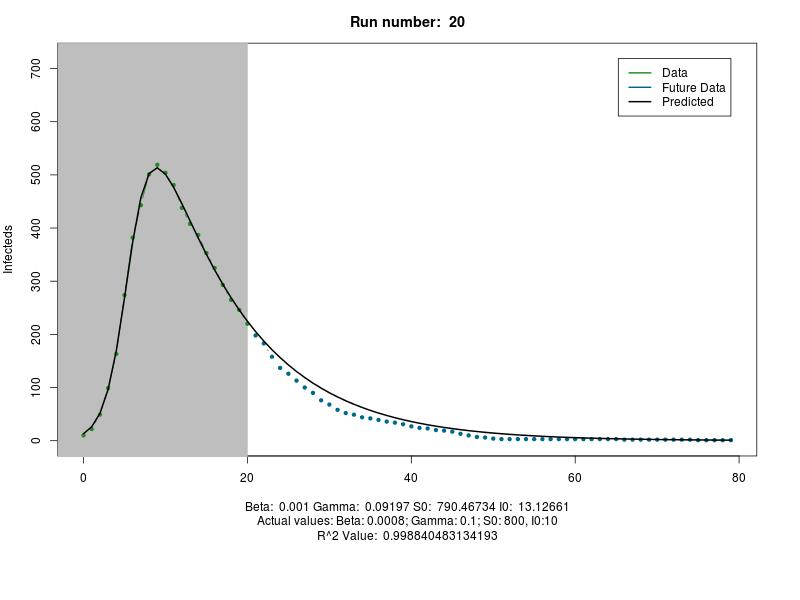
\includegraphics[width=8cm]{images/siri0_20}
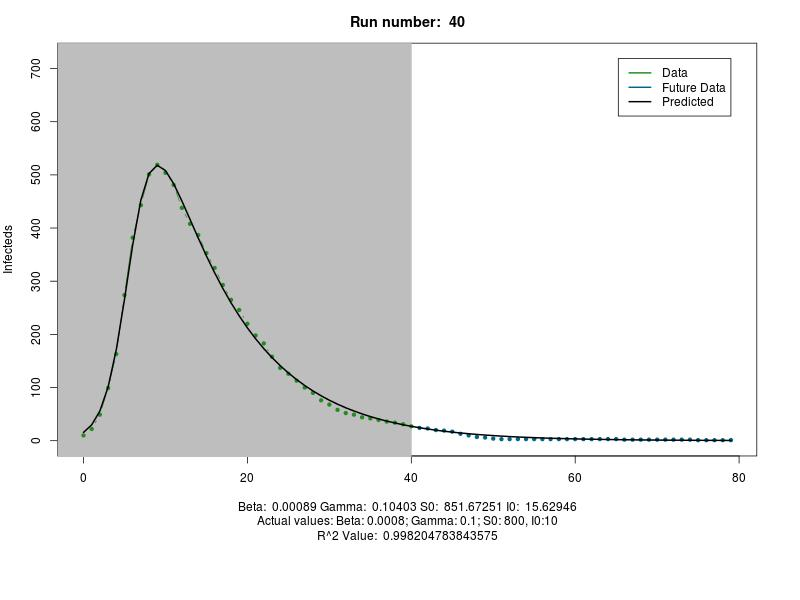
\includegraphics[width=8cm]{images/siri0_40}
\caption{Iterative model fitting over time using least squares
  minimisation. I0, S0, beta and gamma unknown.}
\label{fig:siri0}
\end{figure}
\end{centering}


\begin{figure}
  \centering
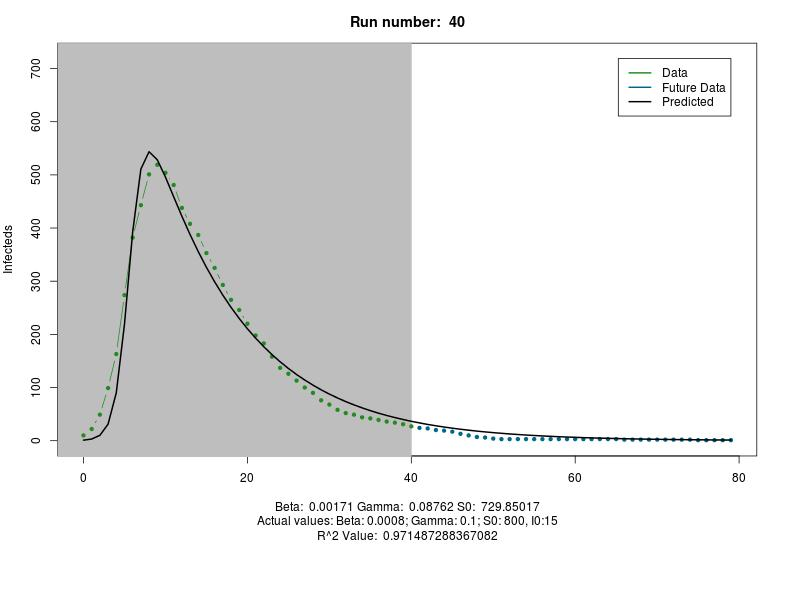
\includegraphics[width=10cm]{images/siri0_unknown}
\caption{Goodness of fit reduced when inaccurate parameter assumptions
  are made.}

\label{fig:siri0wrong}
\end{figure}

\subsection{C++ Implementation}
Although the implementation in R provides a simple and relatively quick
fitting framework, it depends heavily on independently provided
packages. By implementing the fitting framework from scratch, we are
able to address any potential bottlenecks to performance. Furthermore,
it has been found that C++ is much faster than R in modelling
tasks.\cite{languagespeeds} On the flip
side, the lack of available methods imposes a significant cost in
terms of coding time on the project. A significant contribution of this project
is the implementation of model fitting framework from scratch using a
generalisable, objected oriented approach, allowing for the easy
addition of candidate epidemic models. Figure~\ref{fig:uml}  depicts a simplified
UML diagram of the object oriented model fitting framework.


\begin{figure}
  \centering
 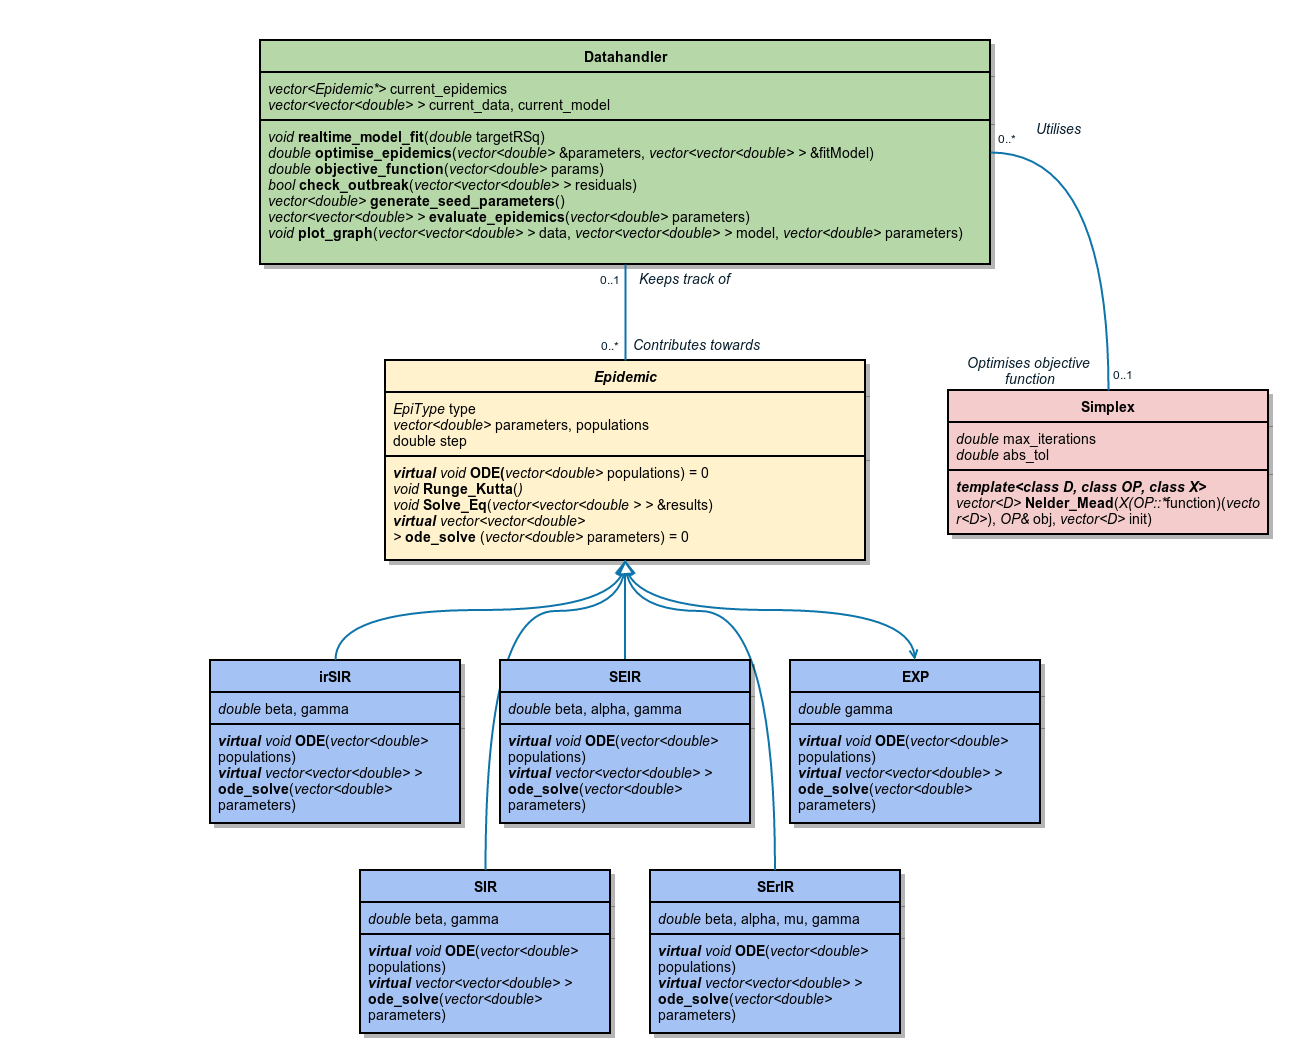
\includegraphics[width=15cm]{images/uml}
\caption{UML diagram of the model fitting framework}
\label{fig:uml}
\end{figure}

The Datahandler class keeps track of the currently available data,
best fitting parameters, current model and currently active
epidemics. The fitting procedure is initiated with a desired fit
level, and the Datahandler proceeds to manage the overall fitting
process. An objective function is formed by solving and summing the
ODEs for each active epidemic, and calculating the SSE against the
available epidemic data. This objective function is passed to the
Simplex class, which carries out the Nelder-Mead algorithm to return
an optimised set of parameters. Note that the Epidemic class is an
abstract class, with each sub class having its own set of parameters
and set of ODEs. The Epidemic class also holds the Runge Kutta method
for solving a given set of ODEs. This allows the framework to be easily extendible to
include additional types of candidate model. The Datahandler class
also manages the analysis of model fit and the plotting of any desired
graphs through the use of Gnuplot. Figure~\ref{fig:sirc} shows the output of the
iterative fitting procedure on synthetic data, where beta, gamma and
S0 are assumed to be unknown.

\begin{figure}
  \centering
  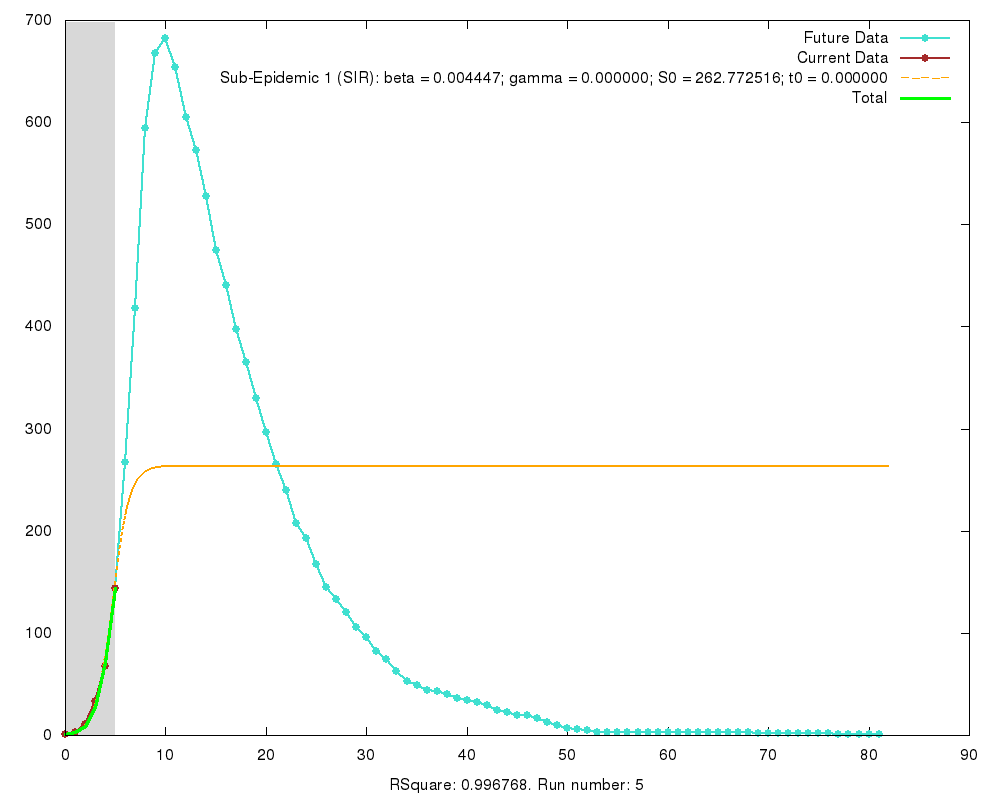
\includegraphics[width=8cm]{images/output5}
  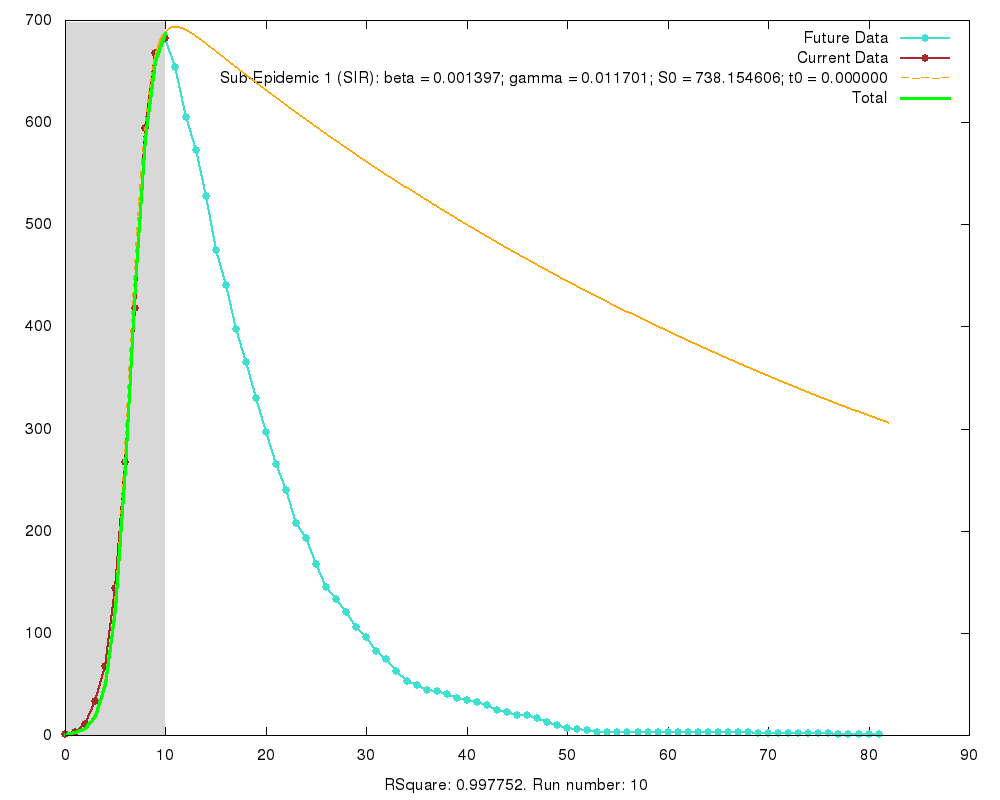
\includegraphics[width=8cm]{images/output10}
  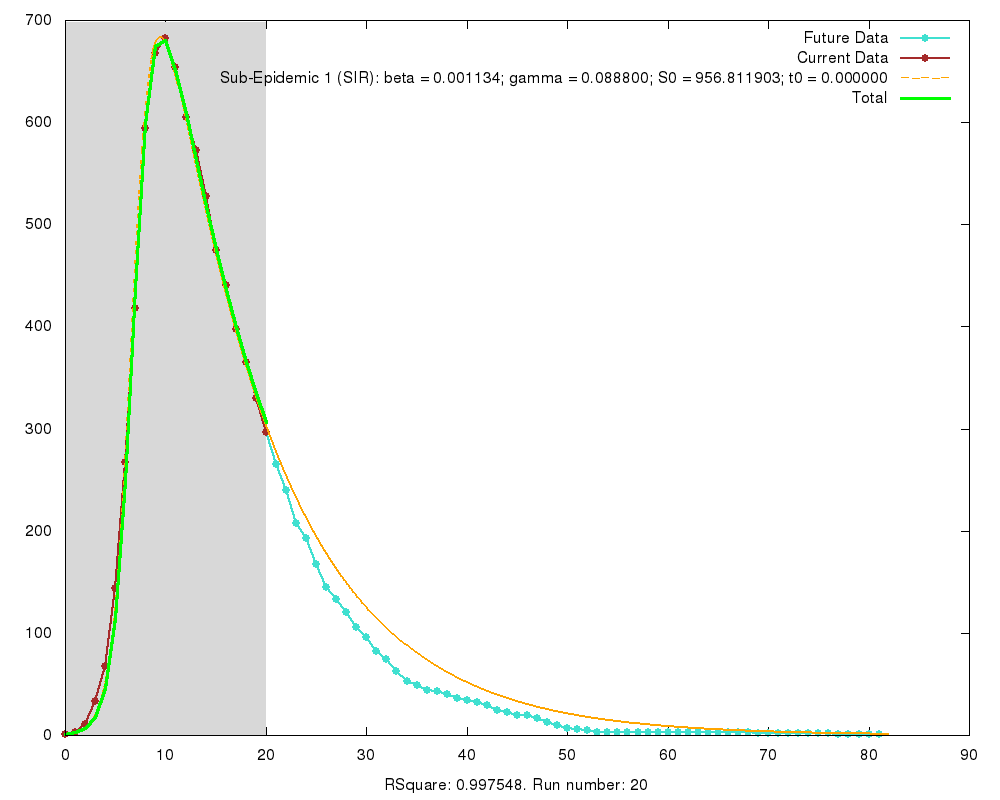
\includegraphics[width=8cm]{images/output20}
  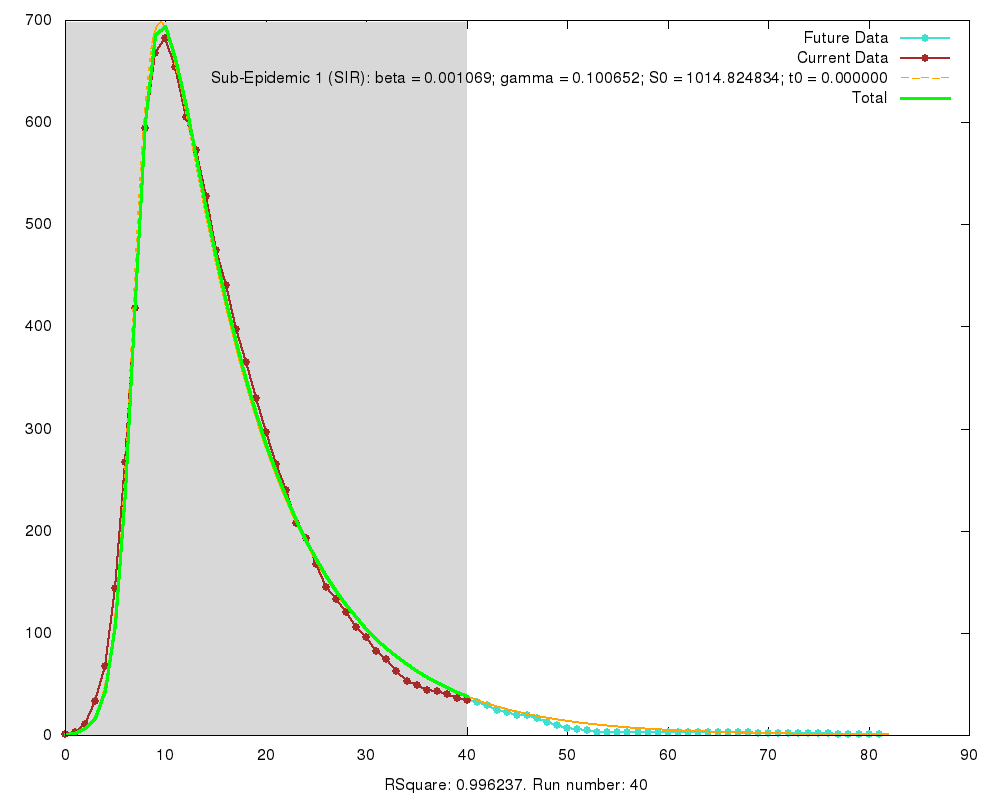
\includegraphics[width=8cm]{images/output40}
\caption{Graphical output of the C++ single model fitting
  framework. Beta = 0.001, gamma = 0.1, S0 = 1000, I0 = 1}
\label{fig:sirc}
\end{figure}


\section{Alernative Candidate Models}

The generalised C++ implementation allows for alternative candidate
models to be fit to our epidemic data. In classical epidemiology, many
infectious diseases are better explained by adaptations of the
\emph{SIR} model. For example, The HIV virus is best explained by the
\emph{SIS} model, where infected individuals do not recover but rather
return to the susceptible compartment.\cite{vynnycky} Similarly, some online epidemic
phenomena have been shown to be better described by an adaptation of
the \emph{SIR} model known as the \emph{irSIR} model, which suggests
that the recovery rate is additionally dependent on the number of
recovered individuals (as themes become `out of
fashion').\cite{cannarella} As discussed in section BACKGROUND, it has
also recently been proposed that online viral trends might spread as either gradual
``growth'' or sudden ``spike'' epidemics, depending on whether the
trend is spread slowly through social networks, or rapidly through
mass exposure. An improved model fitting framework would
therefore allow for the selection of a best fitting candidate model
from a list of potential models.

\subsection{Additional Models}
The present fitting framework considers the SIR and SEIR as initially described
in classical epidemiology.\cite{vynnycky} We also include the Exponential Decay model
to represent a ``spike'' epidemic and the irSIR mdoel as proposed by
Cannarella et al.\cite{cannarella} Furthermore, we propose a novel
adaptation of the SEIR model named the SErIR model. In this model, we
consider the number of exposed individuals rather than the number of
infected individuals as our population of interest. The rationale
behind this is that in
online phenomena, an individual is recorded as having seen or viewed a
video regardless of whether or not they are actively spreading the
epidemic. Furthermore, this model adds an additional parameters,
$\pi$, which represents the rate at which individuals who are exposed
to the `infection' move to the recovered compartment without spreading the infection.

\begin{figure}
\centering
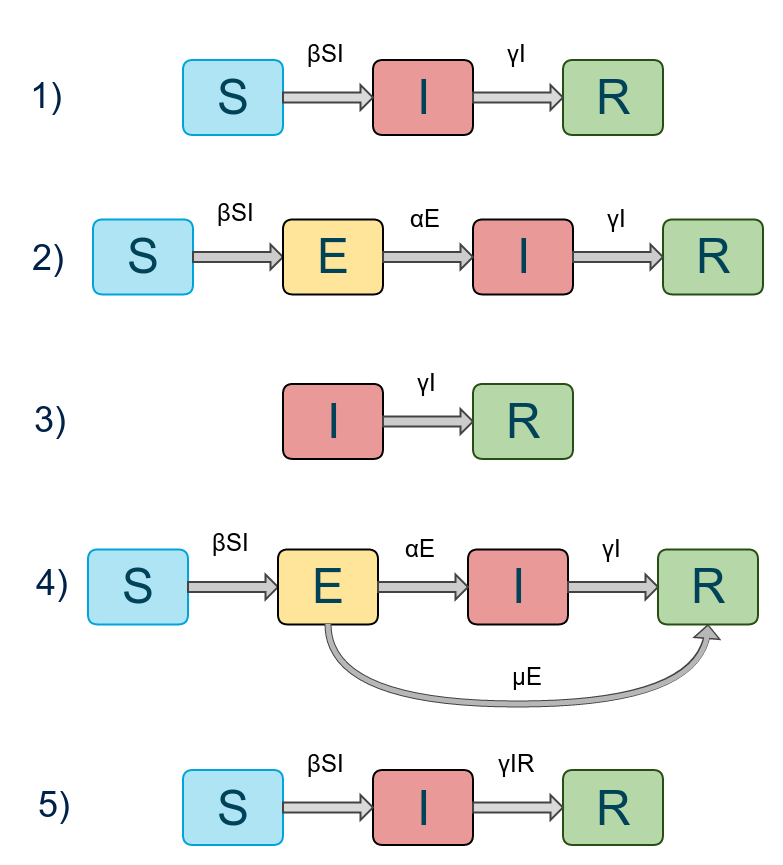
\includegraphics[width=16cm]{images/models}
\caption{1) SIR model. 2) SEIR model. 3) Exponential decay model. 4)
  Modified SErIR model. 5) irSIR model}
\end{figure}

\newpage
\begin{framed}
{\begin{center}{\bf Box 5: Candidate Epidemic Models}\end{center}}
In addition to the \emph{SIR} and \emph{Exponential Decay Model}
described in Box 2, we include the following epidemic models in our
fitting framework:

{\bf The irSIR Model}\\
Originally proposed by Cannarella et al., the \emph{irSIR}
model is an adaptation of the \emph{SIR} model to consider that the
rate of recovery depends on the number of recovered
individuals. The classic \emph{SIR} model considers that infected
individuals recover with a set rate, $\gamma$ as they fight off the
infection. The idea behind the irSIR model is that an individual is
more likely to recover from an infection if they come into contact
with an already recovered individual. For example, Cannarella et
al. suggest that individuals are more likely to stop using a social
network site as overall usage decreases. The \emph{irSIR} model has the following parameter vector and set of
equations:
\begin{equation}
\centering \theta^{(i)} = [I_0^{(i)},
  S_0^{(i)}, \beta^{(i)}, \gamma^{(i)}]
\end{equation}
\begin{centering}
\begin{equation}
	\begin{split}
	&\frac{dS}{dt} = -\beta IS, \\
	&\frac{dI}{dt} = \beta IS - \gamma IR, \\
	&\frac{dR}{dt} = \gamma IR
	\end{split}
\end{equation}
\end{centering}\\
{\bf The SEIR Model}\\
The \emph{SEIR} is another simple adaptation of the \emph{SIR} model
that aims to better describe the course of a disease. Rather than
transitioning from susceptible to infected immediately, many diseases
go through a long incubation period before the infected individual
becomes infectious.\cite{aron} This incubation period is described by
the parameter $\alpha$, where $1/\alpha$ is the mean latent period of
the disease. The \emph{SEIR} model has the following parameter vector
and set of equations:
\begin{equation}\centering\theta^{(i)} = [I_0^{(i)},
  S_0^{(i)}, \beta^{(i)}, \alpha^{(i)}, \gamma^{(i)}]\end{equation} 
\newpage
\begin{centering}
\begin{equation}
	\begin{split}
	&\frac{dS}{dt} = -\beta IS, \\
        &\frac{dE}{dt} = \beta IS - \alpha E, \\
	&\frac{dI}{dt} = \alpha E - \gamma IR, \\
	&\frac{dR}{dt} = \gamma IR
	\end{split}
\end{equation}
\end{centering}\\
{\bf The SErIR Model}\\
A novel candidate model proposed here is the \emph{SErIR} model; an
adaptation of the SEIR model that takes into account incomplete infection
spreading. Whereas individuals affected by an infectious disease will
invariably spread the infection upon contact, individuals that are
exposed to online viral phenomena might not go on to become
spreaders. Furthermore, the measure interest becomes the `exposed'
rather than `infected' compartment, as non-spreaders will contribute
towards the data of interest. Consider the example where an individual
views a \emph{YouTube} video, but does not go on to `share' the link
with anyone else. We introduce the parameter, $\pi$ to describe the
rate at which individuals move from the exposed to the recovered
compartment, where $1/\pi$ might be termed the ``ignoral rate''. The
\emph{SErIR} model has the following parameter vector and set of
equations:
\begin{equation}\centering\theta^{(i)} = [I_0^{(i)},
  S_0^{(i)}, \beta^{(i)}, \alpha^{(i)}, \pi^{(i)}, \gamma^{(i)}]\end{equation} 
\begin{centering}
\begin{equation}
	\begin{split}
	&\frac{dS}{dt} = -\beta IS, \\
        &\frac{dE}{dt} = \beta IS - (\alpha + \pi)E, \\
	&\frac{dI}{dt} = \alpha E - \gamma IR, \\
	&\frac{dR}{dt} = \gamma IR + \pi E
	\end{split}
\end{equation}
\end{centering}

\end{framed}

Figure~\ref{figure:candidates} shows the trajectories of the various
candidate models when seeded with similar parameters. As individuals
move out of the compartment of interest at a greater rate (namely in
the \emph{irSIR} model), the peak becomes much lower. Furthermore, the
introduction of an incubation period as in the \emph{SEIR} and
\emph{SErIR} models delays the peak of the epidemic.

\begin{figure}
\centering
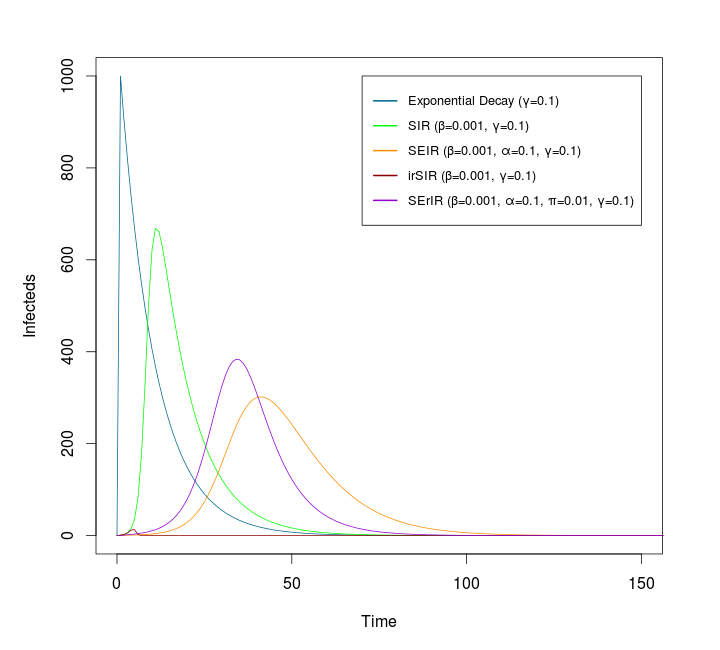
\includegraphics[width=16cm]{images/candidates}
\caption{Dynamics of candidate models with similar parameters and
  starting susceptible population of 1000}
\label{figure:candidates}
\end{figure}

\subsection{Selecting a Model}
The implementation described here allows the user to either fit a
specified epidemic type to the set of data. All relevant
transition rate parameters (eg. beta, gamma) and S0 are included in the
optimisation process, and we allow the user to optionally include I0
as an unknown parameter. The user may also decide to allow the fitting
framework to select the best fitting model for the data. In this case,
the framework attempts to fit each candidate model and tracks the best
fitting result, settling on the candidate model that best describes
the data. This process is not as simple as choosing the model
with the best R Square value. The shape of models with more parameters
is much more adaptable by nature, as the increased number of
parameters results in more inflection points. As all of the candidate
models are extensions of the \emph{SIR} model, the more complex models
(\emph{SEIR}, \emph{SErIR}) will tend to be selected simply due to
their increased complexity. To prevent this overfitting, the relative
model complexity must also be taken into consideration when selecting the best candidate model.

The aim of the candidate model selection procedure is therefore to
select the simplest model that provides a good fit to the data. A
heuristic approach to this problem is to select the model with the
fewest parameters that provides a sufficiently good fit. When
considering which model to add, we first check the R Square value for
each model type and only consider those models that provide a fit
above a pre specified threshold. If more than one model provides a
sufficiently good fit, we choose the model with the fewest
parameters. If two or more models have the same number of parameters
and provide a sufficiently good fit, then we are able to choose the
with the highest R Square value. 

A formal measure of the above heuristic is known as the \emph{Akaike
  information criterion}, or \emph{AIC}.\cite{burnham} Based on information theory, the \emph{AIC} is a measure
of statistical model quality for a given set of data that takes into
account both goodness of fit and model complexity. In general terms, the \emph{AIC}
value of a model is defined as:
\begin{equation}
AIC = 2k - 2ln(L)
\end{equation}
where $k$ is the number of free model parameters, and L is the maximised
likelihood function. The preferred candidate model is that with the
minimum \emph{AIC} value, which therefore minimises information loss. As we are only interested in the comparative
\emph{AIC} values, we can use the $\delta$\emph{AIC} value between two
models. Furthermore, we can also make adjustments for small sample
sizes, as is the case with our epidemic data early on in the fitting
procedure. This \emph{AICc} puts a greater penalty on complex models
than the basic \emph{AIC} score, and is defined as:
\begin{equation}
AICc = -2ln(L) + 2k + \frac{2k(k+1)}{n - k - 1}
\end{equation}
In the scenario where we use the residual sum of squares as our
objective function value, we use the following \emph{AIC} definition:
\begin{equation}
AIC = nln(RSS/n) + 2k
\end{equation}

where $n$ is the number of data points and $RSS$ is the residual sum
of squares.

In terms of implementation, we calculate the \emph{AICc} value for
each candidate model and track the candidate model with the lowest
\emph{AICc} value. Once all candidate models have been considered, the
final model with the lowest \emph{AICc} value is chosen as the best
fitting candidate model. As the first window of data points might not
be representative of the entire data set, we perform this selection
every 10 data points to ensure that the best model is chosen in light
of recent data. 

\section{Maximum Likelihood Based Estimation}
An alternative to least squares based fitting is the use of Maximum
Likelihood Estimation (MLE) as an objective function. The theory  ,

\chapter{Synthedemic Modelling}
\label{ch:multi}
The classic epidemic model brings to mind images of a single curve
with a single peak. When measuring the spread of a single infectious
disease within a closed population, this is often a realistic
characterisation. For example, the number of people in London infected
with a new strain of flu virus might resemble this curve. 

Recent work has highlighted the limitations of the single epidemic
based approach in characterising certain epidemic phenomena, particulary with
regards to viral internet trends.\cite{marily2013, marily2014} A
recent adaptation of the field of \emph{synepidemiology} termed
\emph{synthemics} has been proposed as a potential avenue of further
research. The key challenges of the synthedemic modelling procedure are to
identify the number of underlying epidemics, to identify when these
sub epidemics start, and to identify the type of epidemic model that
best describes each sub epidemic. Furthermore, as the number of
included sub epidemics increases, so to do the number of parameters to
be optimised the corresponding parameter search space. 

In this section we discuss an implementation that aims to address these challenges,
and the particular problems and solutions that arise during the course
of the project.


\section{Identifying Sub Epidemic Start Time}
In the single epidemic fitting framework, it is assumed that there is
only one epidemic in the dataset, and that it can be considered to
have started right at the beginning of the dataset. However, when
considering multiple epidemics simultaneously, it is not possible to
make this assumption, as multiple sub epidemics might start and finish during
the iterative fitting procedure. Furthermore, when multiple epidemics
are progressing simultaneously, it might not be possible to detect the
start of a new epidemic until it is well underway. The start time of
the epidemic therefore might (and probably will not) match the
detection time. The first step in developing a
synthedemic model fitting framework is therefore to implement a means
to detect and record epidemic start times, and to consider how these
start times will be included in the optimisation procedure.



\subsection{Epidemic Detection}
The aim of detecting an epidemic outbreak is to determine when the
level of infected individuals has begun to rise above the expected
baseline level. In most cases, there will be a certain number of
background infecteds that are endemic in the population. For example,
consider that there will be some individuals infected with flu
throughout the year. The first step in our detection procedure is
therefore to establish a baseline level, taken as the mean of the data
points up until detection.

At each time point, residuals are generated from the difference
between the current best fitting model and the available data. If
there are no active epidemics, the best fitting model is taken as the
baseline level. We then check the latest residual for signs of an
epidemic outbreak. If the latest residual lies a certain number of
standard deviations away from the mean of the previous residuals, then
we suspect that an outbreak might have occured. As the detection
procedure is dependent on the variation in the past residuals, the sensitivity of
outbreak detection is dependent on the noise of the data itself. If
the data set shows very low variation, then the standard deviation of
the residuals will be low; resulting in a low detection
threshold. Similarly, if the standard deviation is very high (as might
be the case with real world data), then the threshold will be very
high. In terms of implementation, we therefore couple the residual
detection threshold with a measure of the current model fit. If the
current model fit is less than a certain value, then the model fit has
deteriorated sufficiently to consider the addition of another sub
epidemic.

Although the above detection method is a sound heuristic approach, the
dependence on the quality of the data means that detection time may
be inaccurate. When the outbreak begins gradually, the change to the
mean and standard deviation of the residuals may be small enough that
the latest residual is never outside of the detection
range. In epidemic outbreaks of infectious diseases, proxies for
detection might be used in place of analysing the epidemic data
itself. Please refer to section EVALUATION for further discussion of
alternative approaches to outbreak detection.


 For example, the World Health Organisation gathers reports and
rumours of suspected outbreaks from various informal sources and
national health organisations in the hopes of
investigating and catching a potential outbreak as early as
possible. CITE WHO. One tool used by the WHO is the Global Public
Health Intelligence Network



\subsection{Optimising Epidemic Start Times}
Once an epidemic outbreak has been detected, the next challenge is to
find the actual start time of the epidemic. Simply using the detection
time of the sub epidemic as the actual start time is unsatisfactory,
as it assumes that the detection procedure will pick up a new outbreak
as soon as it starts. Some sub epidemics will be hidden within larger
outbreaks and may not be detected until well into their course. 

An initial naive approach to finding the start time of each sub
epidemic might be to consider each possible combination of epidemic
start times. If we consider every possible start time, this would
result in \emph{n}
optimisations for a single epidemic, where \emph{n} is the number of
data points currently available. As soon as multiple epidemics are
considered simultaneously, this quickly becomes infeasible as the
complexity increases with the number of sub epidemics. An heuristic adaption to this is to only consider a subset of start
time combinations. For example, we can consider only the start times
within a window of the detection time, and assume that the ordering of
start times does not matter. This results in \emph{tCn} combinations
of start times, where \emph{t} is the number of time points under
consideration, and \emph{n} is the number of epidemics to be
fit. 

Although such heuristics  might provide a
conceptually simple optimisation approach, they avoid the problem of
including $t_0$ in the optimisation procedure directly. Doing should
allows for the start time of each sub epidemic to be found
precisely. Furthermore, doing so allows us to consider the start time
as a continuous variable, making the model fit much more accurate. We
therefore chose to initially include $t_0$ as an unknown parameter in
the optimisation procedure. Giving the Nelder Mead algorithm a
completely random time as a seed value risks producing an extremely
high initial SSE value. We therefore use the detection time minus a
small value (to account for delayed detection) of the epidemic
as the seed value for the optimisation procedure. 

\section{Initial Approach}
The initial approach aims to iterate over a set of epidemic data,
where it is not assumed that there is an ongoing epidemic from the
start. We include the transition parameters, beta and gamma, as well
as S0 and t0 in the optimisation procedure. As in the single fitting
framework, at each time point we produce random seed values and choose
the best run from ten independent as the best fitting model. T0 is
seeded as the detection time of the epidemic. We first fit the
currently known \emph{k} epidemics, and then consider the addition of
an epidemic when the model fit has deteriorated sufficiently and
the latest residual is a certain number of standard deviations away
from the previous residuals' mean. By only adding an additional
epidemic when the model fit has deteriorated sufficiently, we avoid
needlessly overfitting the data when an outlying data point might
falsly suggest the start of a new epidemic.

We initially consider only SIR models, which result in a combined
parameter set of $(\beta^{(k)},\gamma^{(k)},\S_{0}^{(k)},t_0^{(k)})$ to
be optimised. One risk of only considering the addition of epidemics
is that we risk overfitting the data. To avoid this, we also consider the removal of a
sub epidemic at each time point. This is done by removing each sub
epidemic from the current set in turn and reoptimising the remaining
model. If this fit of $k-1$ epidemics is sufficient, we
permanently remove the epidemic from the list.

\subsection{Practicality Considerations}
As the fitting process is a computationally time intensive procedure,
we adhere to the following heuristics to prevent the run time from
becoming infeasible:

\begin{enumerate}
\item Only one epidemic is added or removed at each stage.
\item For SIR epidemics (and sub types in later implementations) we assume that the number if initial infected
  individuals is 1. 
\item For EXP epidemics, the number of infected individuals is
  included as an unknown parameter. A potential simplification of this
  is to use the difference between the current best fitting model and
  the time point at which the epidemic is detected. However, this
  does not allow for the possibility that our current best fitting
  model might not be optimal.
\item The seed time for $t_0$ for SIR type epidemics is taken as the
  detection time minus 10, and searched within the range
  $t-50\leftarrow t$, where $t$ is the detection time.
\item At each time point, we choose the best of 10 independent
  optimisation runs for $k$ epidemics and $k-1$ epidemics, testing the
  removal of all current epidemics to prevent overfitting. When adding
  epidemics, we consider adding each candidate model if the latest
  residual is over three standard deviations away from the mean residual size.
\end{enumerate}

\subsection{Initial Testing}
The multiple epidemic fitting framework was firstly tested using
synthetic data generated by the \emph{GillespieSSA} algorithm in R. To
simulate multiple overlapping epidemics, we run \emph{GillespieSSA}
for each sub epidemic and offset the values by the desired $t_0$;
adding the infected values of each sub epidemic on the corresponding
time points. Two \emph{SIR} models were combined with the following
parameters:

$\beta^1=0.001, \gamma^1 = 0.1, S_0 = 500, t_0 = 10$\\
$\beta^1=0.0008, \gamma^1 = 0.008, S_0 = 800, t_0 = 30$

The initial implementation detected the start of the first epidemic at
$t = 14$, and proceeded to accurately fit the the epidemic. At around
$t = 30$, the second epidemic was detected and added to the
optimisation procedure. The R Square value for the model fit to the
currently known values remains high throughout the fitting procedure
at over 0.99, though it does occasionally fall to around 0.95. This is
likely due to poor initial seed values.

\begin{centering}
\begin{figure}[h!]
  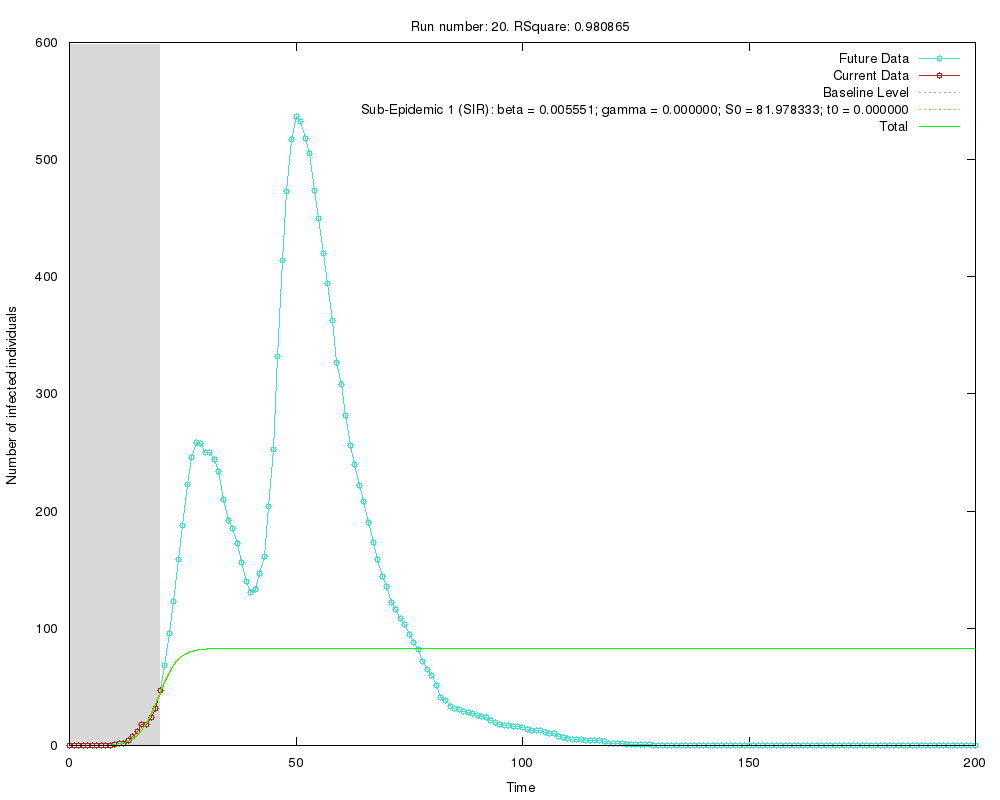
\includegraphics[width=8cm]{images/multi/sirsir1.png}
  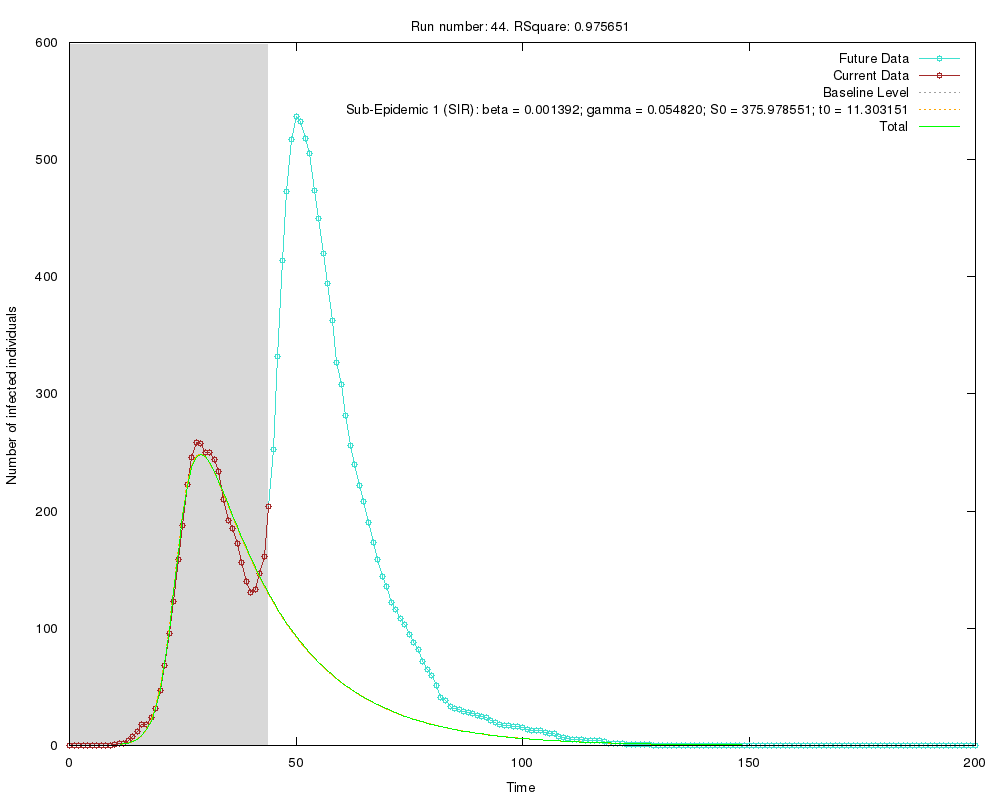
\includegraphics[width=8cm]{images/multi/sirsir2.png}
  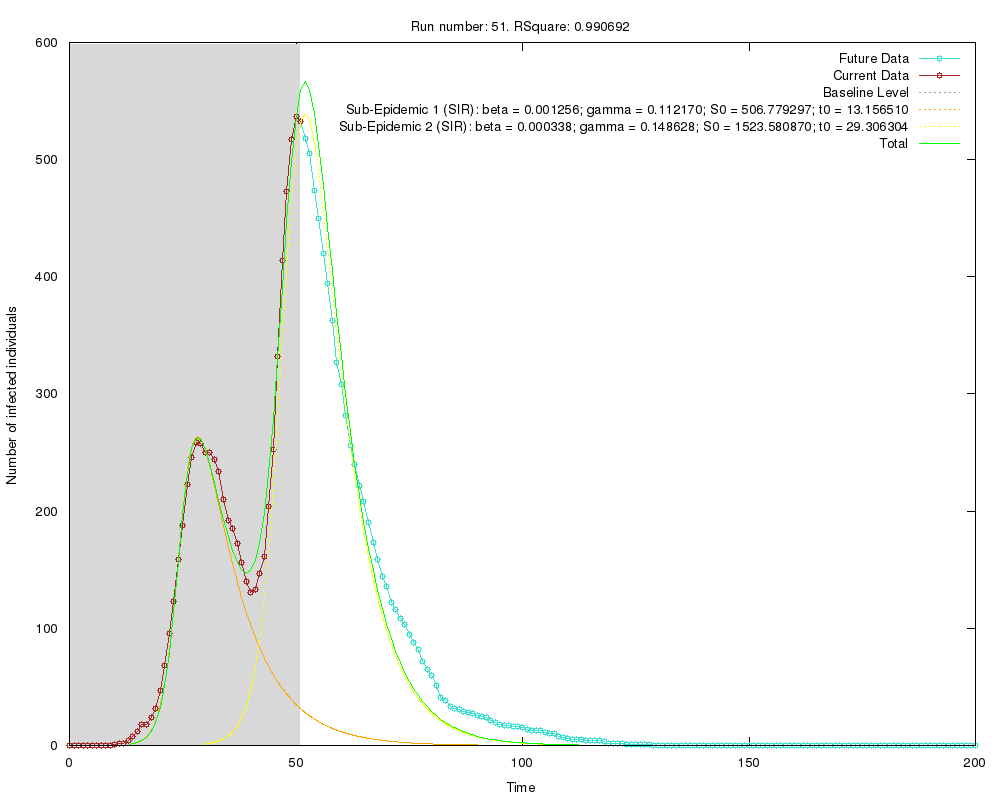
\includegraphics[width=8cm]{images/multi/sirsir3.png}
  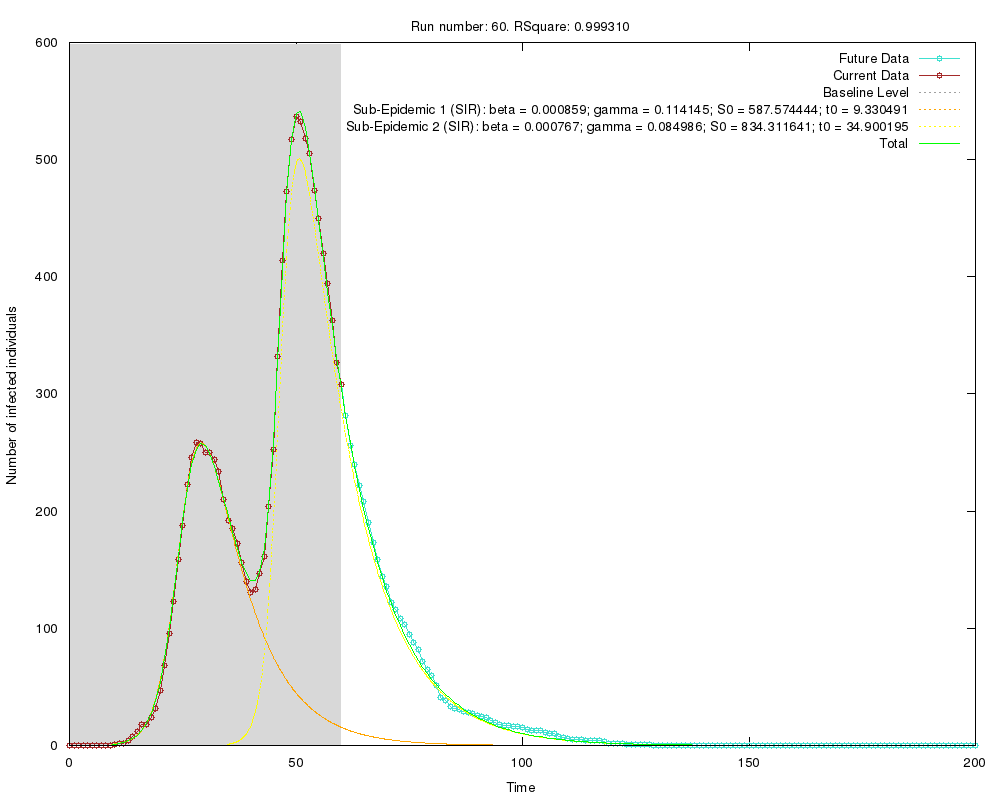
\includegraphics[width=8cm]{images/multi/sirsir4.png}
  \caption{Multiple epidemic fitting procedure on two overlapping SIR models}
\label{fig:sirsir1}
  \end{figure}
\end{centering}

As in the single epidemic fitting framework, a problem that
occasionally occured was that the the optimisation procedure
occasionally tended towards values far outside the range of realistic
values. For example, the optimisation makes $S_0$ very large as it
explores a particular local minimum. Furthermore, the inclusion of
$t_0$ as an additional parameter makes the optimisation procedure much
less stable, particularly when uncertainty in other model parameters
is high. This results in a model fit that is not quite as good as we
might hope, particularly when considering earlier sub epidemics. 


\subsection{Parameter Transformations and Bounding}
A potential way of limiting the space in which the Nelder-Mead
algorithm searches for parameters is to bound the parameters. As
discussed in section SECTION, it is often desirable to transform the model parameters into log space. Another potential transformation that may be applied is through the
use of the \emph{logistic} function. Originally studied in the context
of population growth, maps the parameter search space from between $0$ and $1$
to between $-\infty$ and $+\infty$. The function is
defined as:
\begin{equation}
logistic(x)=\frac{1}{1+e^{-x}}
\end{equation}
The inverse of the logistic function, the \emph{logit} function, can
therefore be used to map the search space of a parameter, \emph{p},
from between $-\infty$ and $+\infty$ to between $0$ and $1$. The logit
function is defined as:
\begin{equation}
logit(p) = log(\frac{p}{1-p})
\end{equation}
The logit function can be modifed to transform the search space from
between $0$ and $1$ to one between $0$ and $max$ as follows:
\begin{equation}
newLogit(x) = \frac{max}{1+e^{-x}}
\end{equation}
with the inverse defined as:
\begin{equation}
newLogistic(x)=log(\frac{x}{max-x})
\end{equation}

 The logic behind this modification can be expanded further to use the logistic function to provide lower bounds as well as upper bounds. As
$x\rightarrow +\infty$, $logit(x)\rightarrow 1$. Similarly, as
$x\rightarrow-\infty$, $logit(x)\rightarrow 0$. We can therefore modify
the logistic function as follows:
\begin{equation}
f(x) = \frac{x_{max}-x_{min}}{1+e^{-x}} + x_{min}
\end{equation}.

We can see that as $x\rightarrow +\infty$, $f(x)\rightarrow x_{max}$,
and as $x\rightarrow -\infty$, $f(x)\rightarrow x_{min}$. By limiting
the parameter search space to a predetermined range of expected
values, we ensure that the optimisation procedure does not get stuck
in a local minimum far away from the actual parameter values. However,
doing so requires us to make assumptions regarding where the real
parameter values might lie. Whilst a good model fit might be produced
within a provided range of parameter values, this fit might be sub
optimal compared to the model produced from a set of entirely
unexpected parameters. 

An alternative, simple approach to bounding parameter values in the
optimisation procedure is to modify the results returned by the
objective function. As the Nelder Mead algorithm transforms parameter
values with the aim of minimising the objective function, we can
direct the parameter search by ensuring that the objective function
returns high values when venturing into an undesirable parameter
space. For example, we can include a simple check of each parameter
with each call of the objective function; returning a high SSE value
if the parameter is outside our desired range. This method was
implemented initially; however, it appeared to result in the Nelder
Mead algorithm returning nonsense values more frequently as it failed
to identify any local minima. This is due to the fact that the
optimisation surface becomes much less smooth, as each check outside
of the specified bounds results in a sudden spike in function value.  

Using the above methodology, we initially add constant limits to $S_0$
and $t_0$; ensuring that $S_0$ stays within the range 100-15000, and
$t_0$ stays within the range of data (typically 0-200). Although this
did improve the stability of the fittnig procedure, it was found that
the range of possible $t_0$ values could be limited further. Rather
than using 0-200, we use a window of time around the detection
time. We use the detection time of the epidemic as the upper bound of
the transformation, and $t-40$ as the lower bound.

\section{Implementation Revision with Parameter Bounding}
Figure~\ref{fig:sirsir2} shows the results of the fitting procedure on
the same two overlapping SIR models usnig logitic bounding on $S_0$
and $t_0$. As in the previous implementation, the fitting procedure
maintains a high R Square value throughout, and accurately detects the
second epidemic. With an effective multiple SIR fitting framework, we
then attempt to consider the addition of an EXP model. As dicussed in
the context of single epidemic model fitting, we add the candidate
model that produces the best model fit in terms of \emph{AICc}
value. For $t_0$ bounding, we use a very narrow optimisation for the
EXP epidemic. Figure~\ref{fig:sirexp1} shows that the framework is able to
accurately detect and fit both the SIR and EXP model throughout the
fitting procedure.


\begin{centering}
\begin{figure}[h!]
  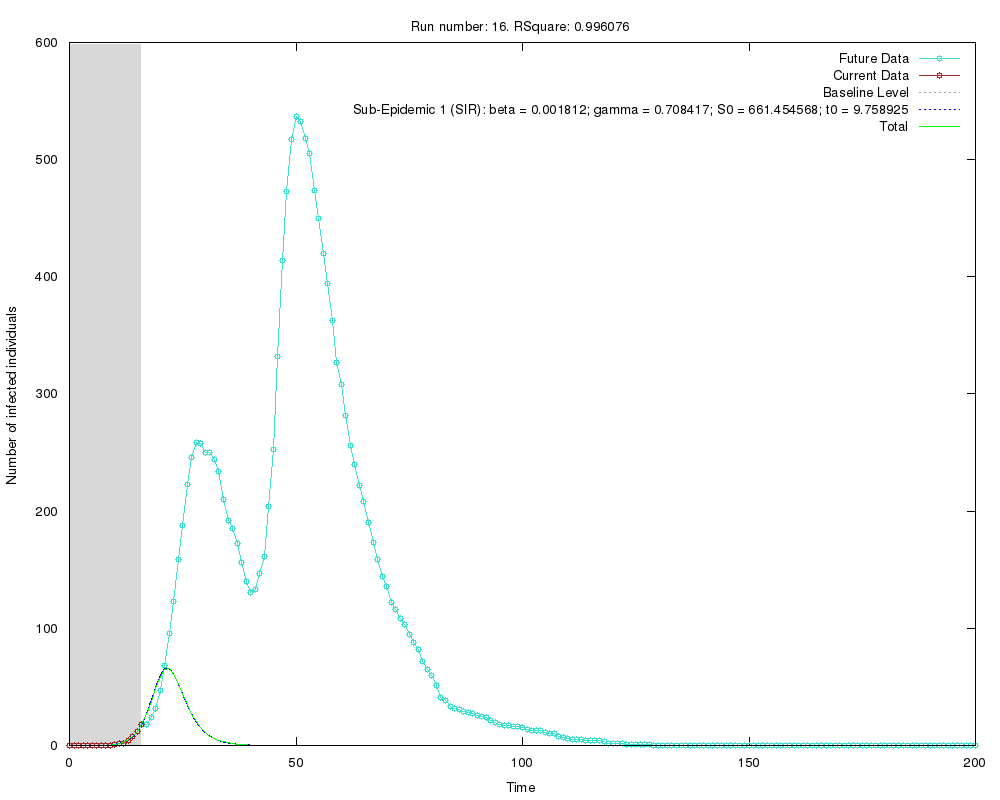
\includegraphics[width=8cm]{images/multi/sirsir6.png}
  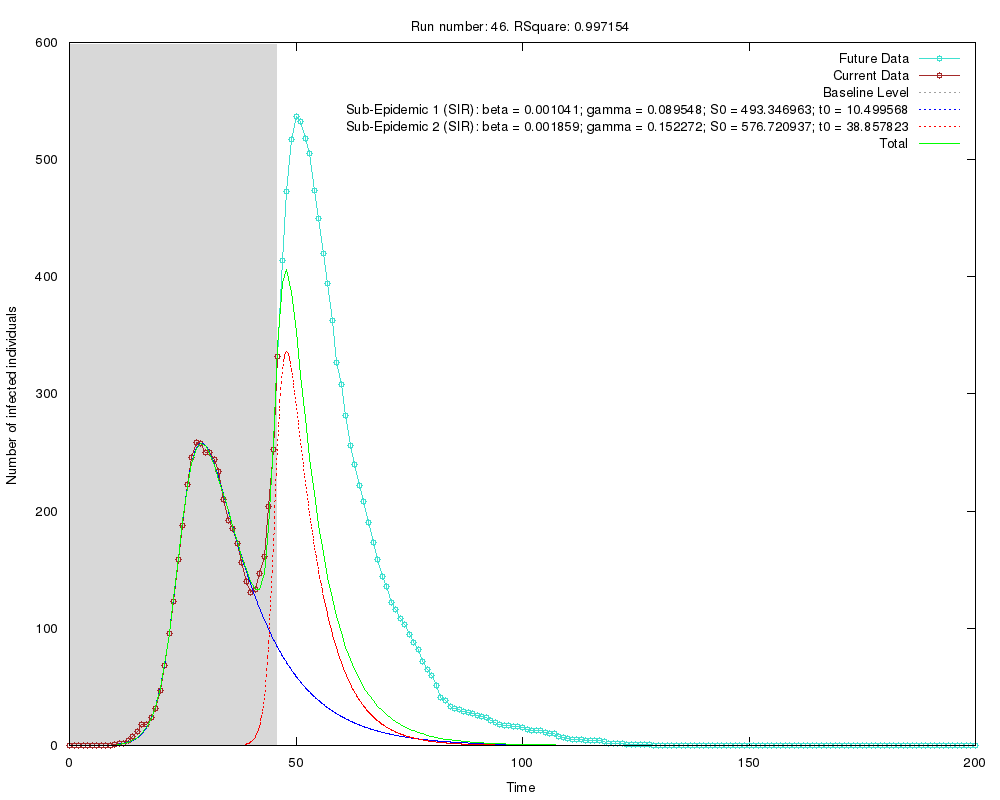
\includegraphics[width=8cm]{images/multi/sirsir7.png}
  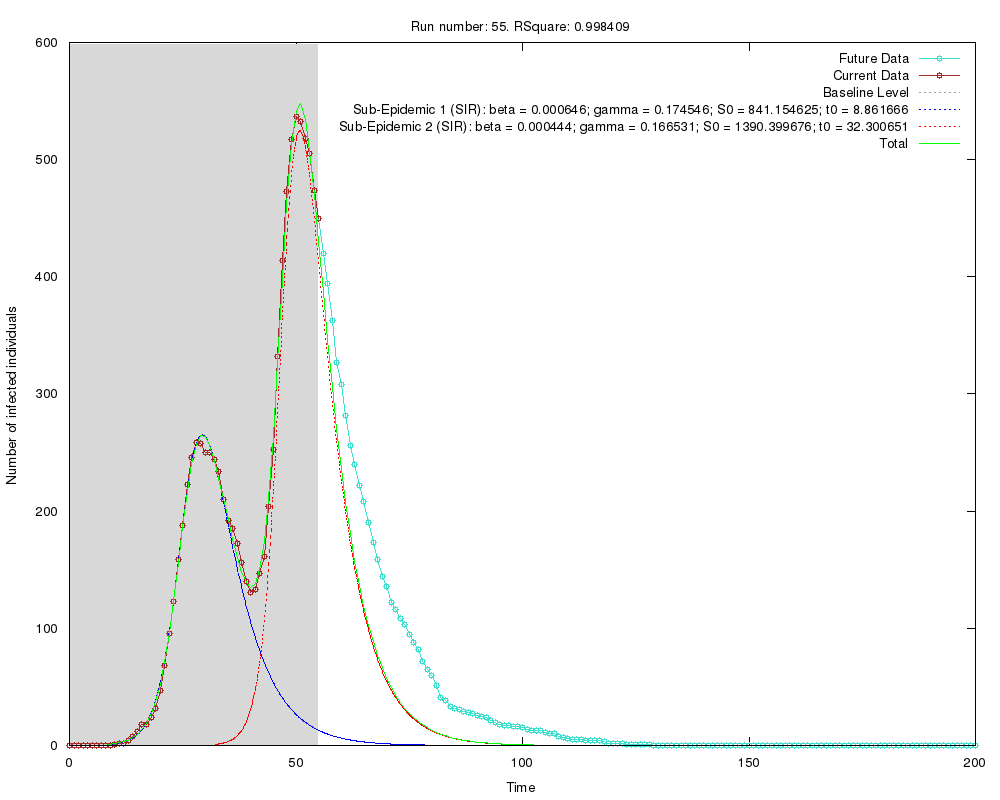
\includegraphics[width=8cm]{images/multi/sirsir8.png}
  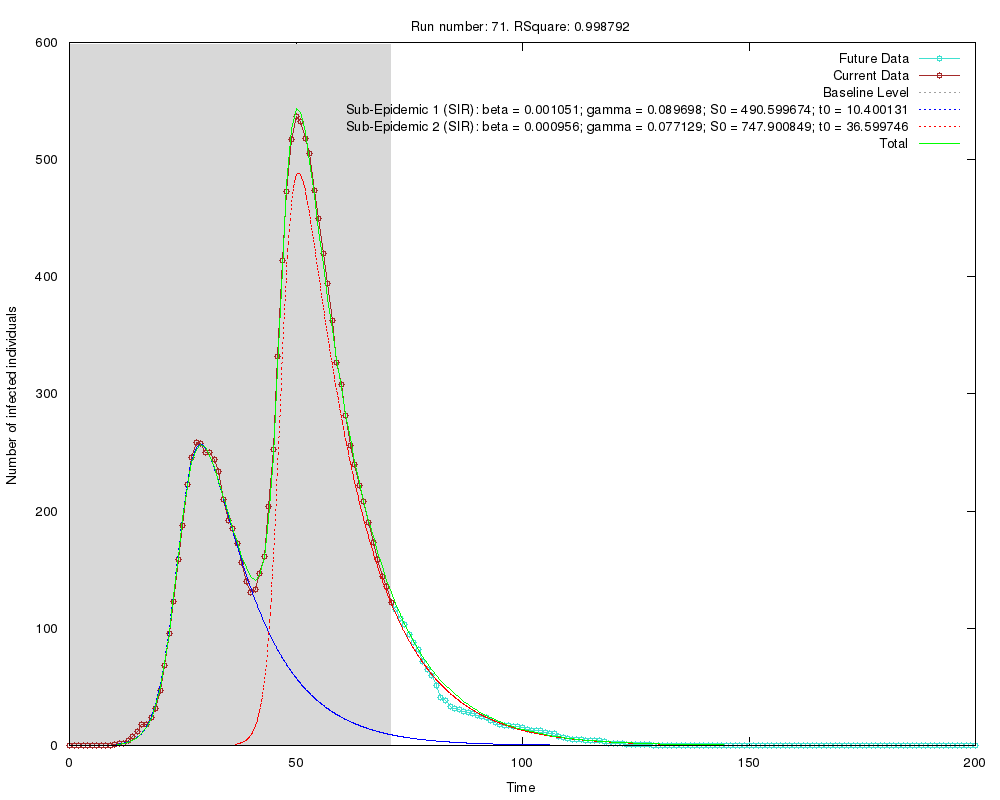
\includegraphics[width=8cm]{images/multi/sirsir9.png}
  \caption{Multiple epidemic fitting procedure on two overlapping SIR
    models with logistic bounding}
\label{fig:sirsir2}
  \end{figure}
\end{centering}


\begin{centering}
\begin{figure}[h!]
  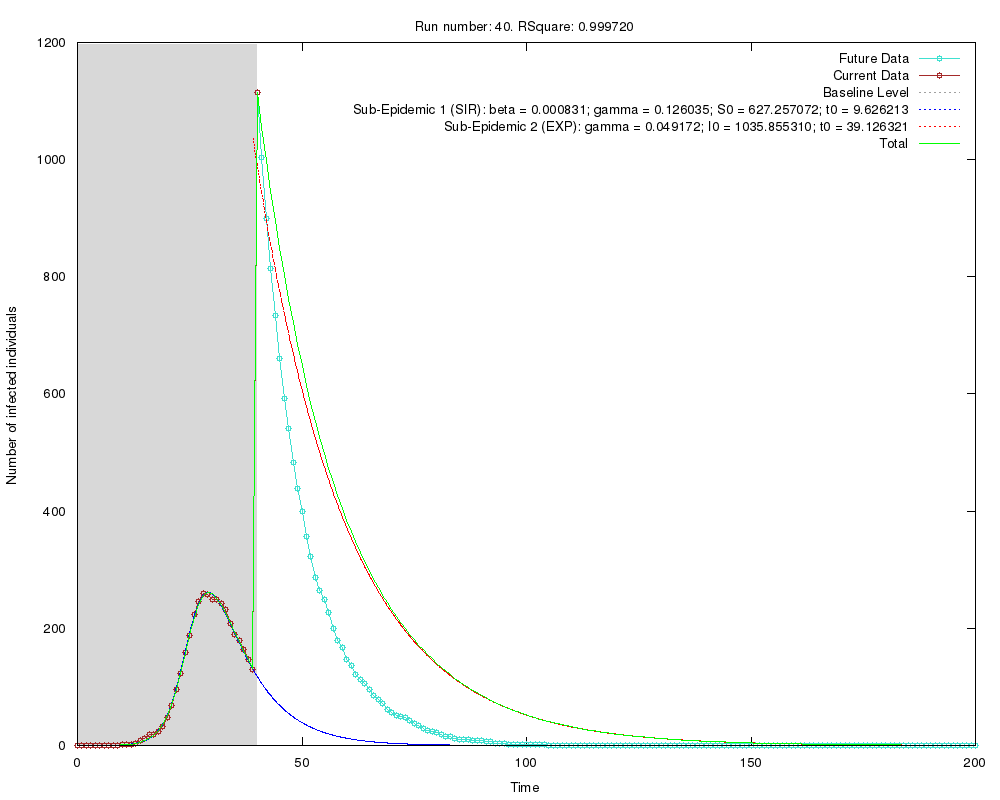
\includegraphics[width=8cm]{images/multi/sirexp1.png}
  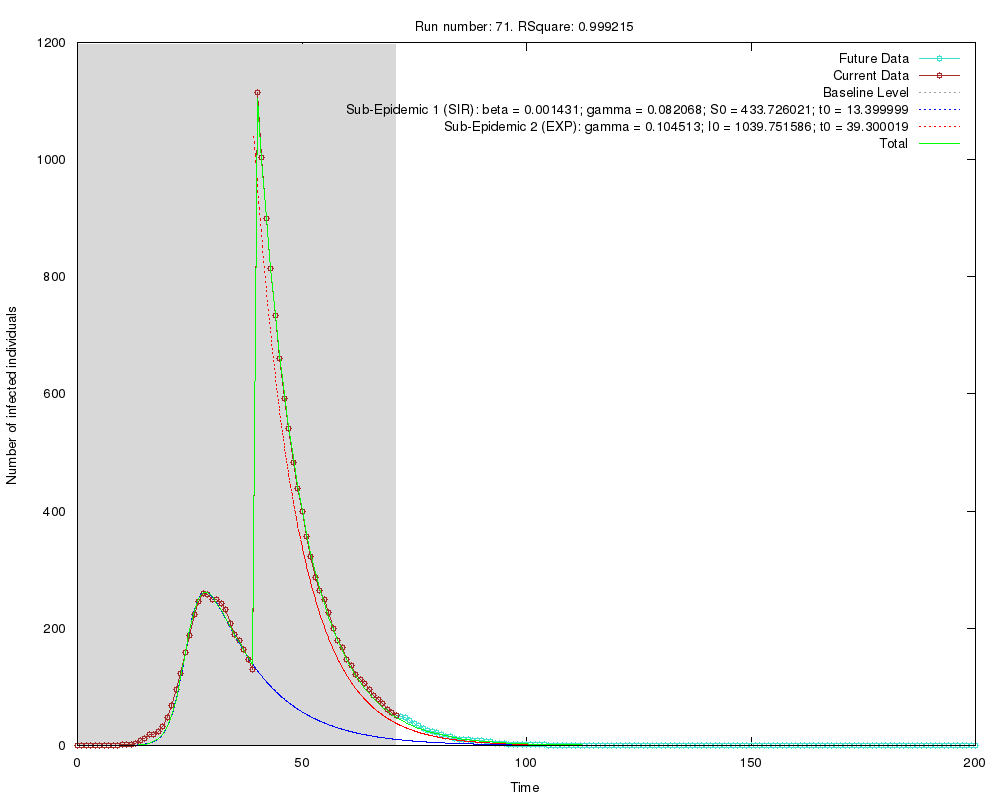
\includegraphics[width=8cm]{images/multi/sirexp2.png}
  \caption{Multiple epidemic fitting procedure on an SIR and EXP models with logistic bounding}
\label{fig:sirexp1}
  \end{figure}
\end{centering}

The true parameters used in figure~\ref{fig:sirexp1} are:

$SIR: beta = 0.001, gamma = 0.1, S_0 = 500, t_0 = 10$ \\
$EXP: gamma = 0.1, S_0 = 1000, t_0 = 40$


\section{Final Implementation}
With a multiple epidemic fitting framework implemented, we then went
on to test our epidemic fitting framework on real epidemic data. To
put the framework to the test, we firstly attempted to characterise
the viral internet sensation, ``Blurred Lines'' by Robin Thicke. To
speed up the fitting process, we only consider SIR and EXP models. We
use the number of \emph{BitTorrent} downloads between As
a first attempt, the model provided a reasonable fit to the data,
characterising the overall shape fairly well. However, as can be seen
in figure~\ref{fig:rt1}, there are a number of shortcomings in the
present approach:

\begin{enumerate}
  \item The characterisation of the first SIR epidemic worsens during
    the fitting procedure, particularly towards the end.
  \item The long term projection of the epidemic varies throughout the
    run. For example, whereas the first graph predicts that there will
    constantly be around 4000 infected individuals, the second graph
    predicts that the epidemic will eventually die out.
  \item The procedure is unable to pick up the epidemic peaks at
    around day 180 and day 220.
\end{enumerate}


\begin{centering}
\begin{figure}[h!]
  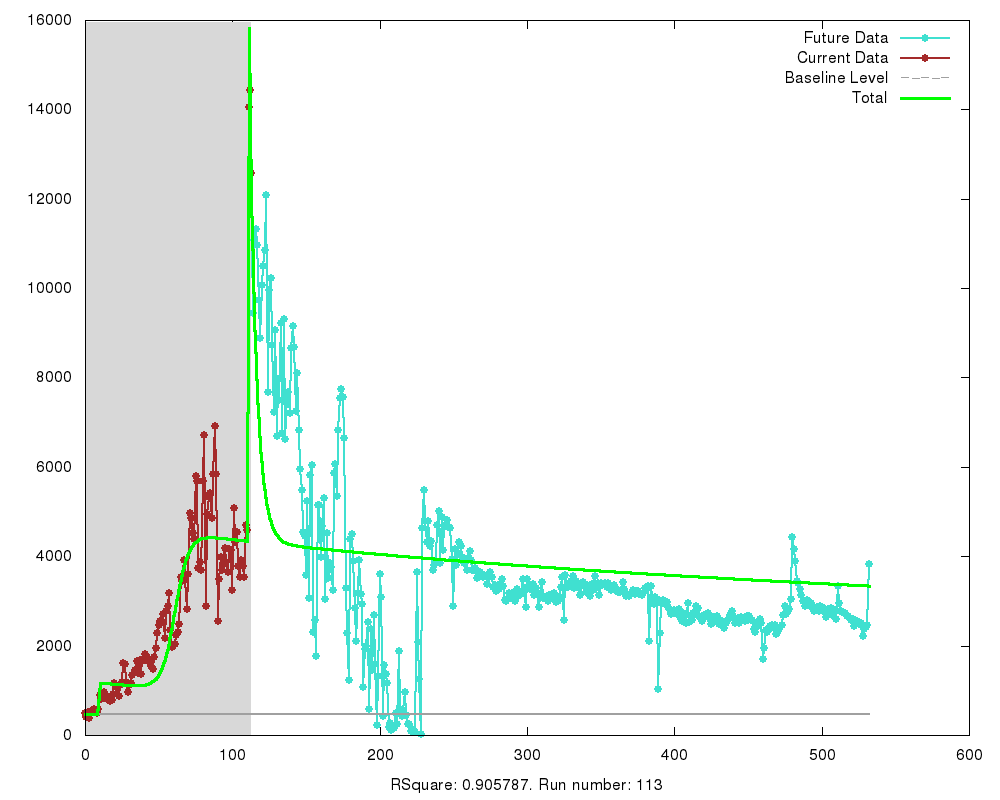
\includegraphics[width=8cm]{images/multi/badrt1.png}
  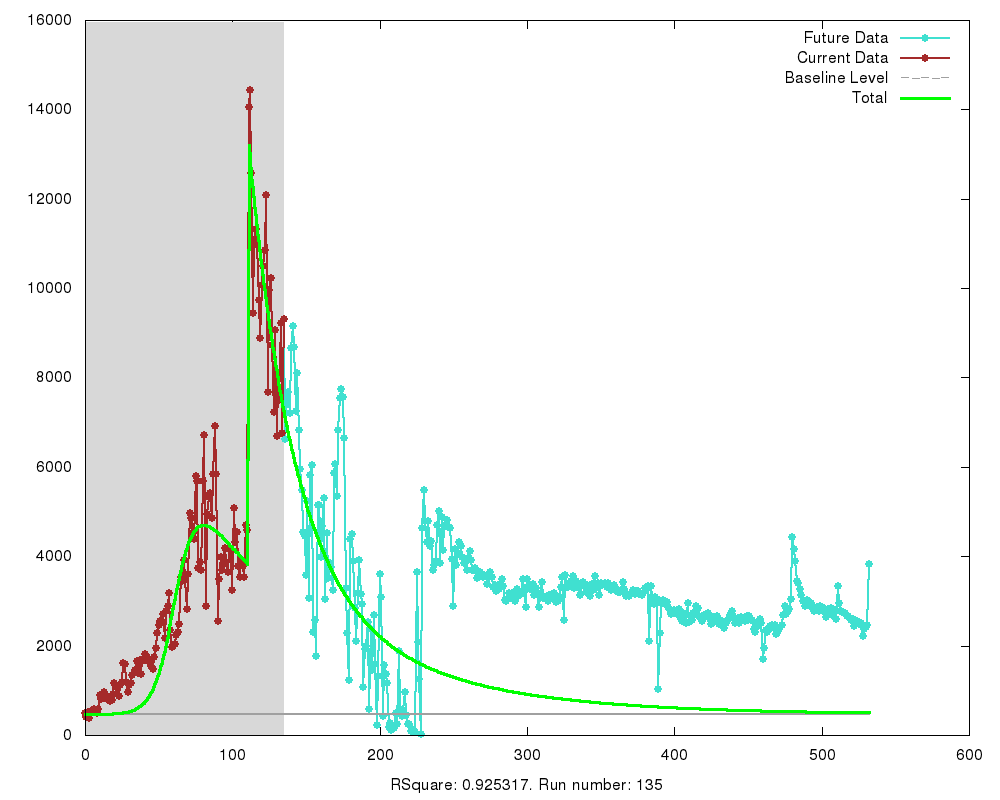
\includegraphics[width=8cm]{images/multi/badrt2.png}
  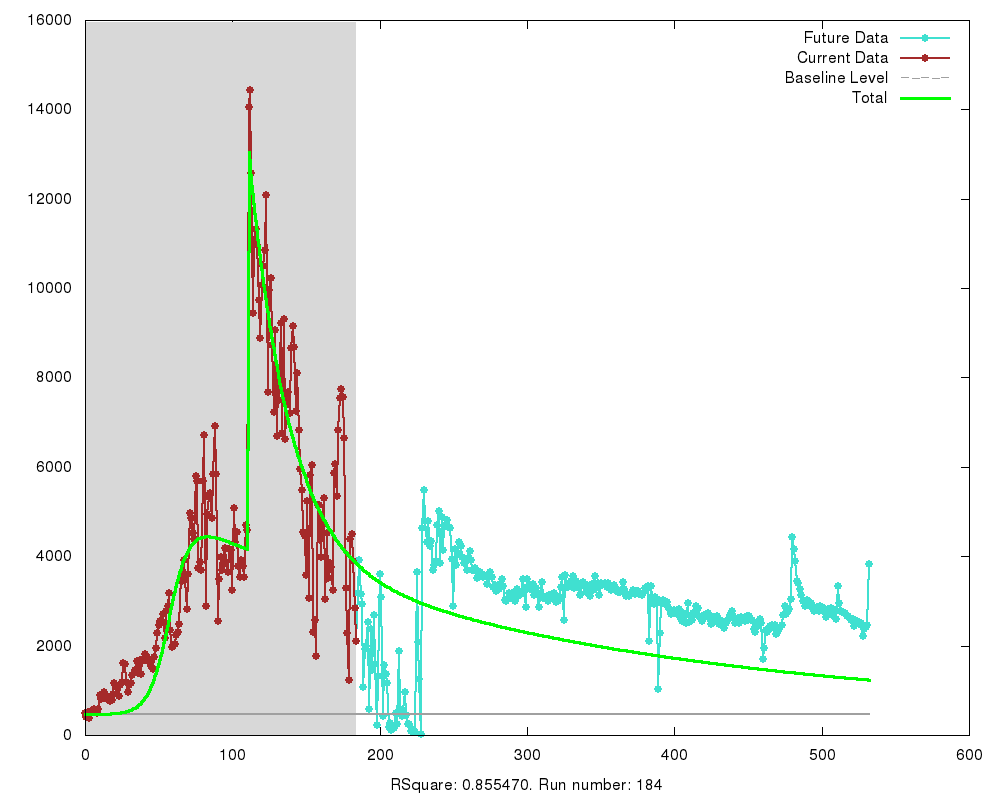
\includegraphics[width=8cm]{images/multi/badrt3.png}
  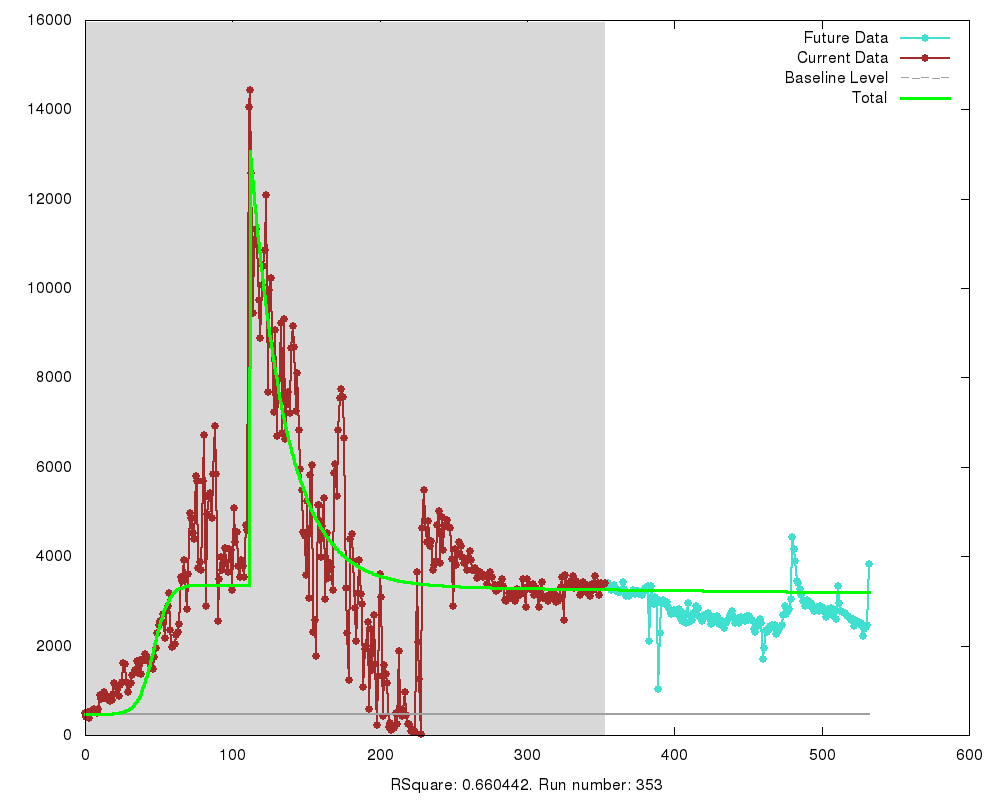
\includegraphics[width=8cm]{images/multi/badrt4.png}
  \caption{Multiple epidemic fitting procedure on the number of
    \emph{BitTorret} downloads of the song ``Blurred Lines'' by Robin
    Thicke. Number of downloads on the y-axis and day on the x-axis}
\label{fig:rt1}
  \end{figure}
\end{centering}

The main reasons for the this instability and inaccuracy can be
attributed to the following:

\begin{enumerate}
\item \textbf{Problem:} Not constraining the transition parameters (eg. beta and gamma)
  results in a number of optimisation runs that do not converge on a
  decent fitting solution. Furthermore, using a potential seed range
  of parameters that are too far from the correct value results in a
  number of unstable runs. For example, if the basic reproduction
  number, $R_0$ is less than one (where $R_0 =\frac{\beta}{\gamma}$),
  then the epidemic will not take off. It was found that seeding the
  optimisation with a high value of $S_0$ often produced non
  convergent runs.\\
  \textbf{Solution:} The seed times of the transition parameters
  should be adapted to ensure that they are within a reasonable
  range. Secondly, we can use the logistic transformation to bound
  these parameters within a sensible range. We also seed $S_0$ with a
  lower than expected value and allow the optimisation algorithm to
  `grow' the value.
\item \textbf{Problem:} The detection threshold for new epidemics is set too high. In
  the above run, we use a threshold R Square value for 0.8, which
  potentially allows for outlying data points to be ignored.\\
  \textbf{Solution:} The target R Square value is increased, and the
  distance to latest residual from the mean of the residuals is
  reduced to two standard deviations.
\item \textbf{Problem:} The time taken to run ten optimisations is
  longer than desirable.\\
  \textbf{Solution:} We investigated the effect of changing the
  scaling parameters in the Nelder-Mead algorithm itself. We initially
  used parameter values of 1.0, 1.0, 0.5 and 0.5 for reflection,
  expansion, contraction and secondary contraction respectively. The
  expansion parameter is particularly troublesome, as it currently
  does not stretch the simplex towards the best vertex. We therefore
  changed these values to 1.1, 1.5, 0.4 and 0.4 respectively, which
  resulted in a significant decrease in optimisation time.
\end{enumerate}

Following the above modifications, the framework was rerun on the
``Blurred Lines'' download data as shown in
figure~\ref{fig:goodrt}. Note that the number of data points is
reduced by taking every fourth data point to reduce run time.

\begin{centering}
\begin{figure}[h!]
  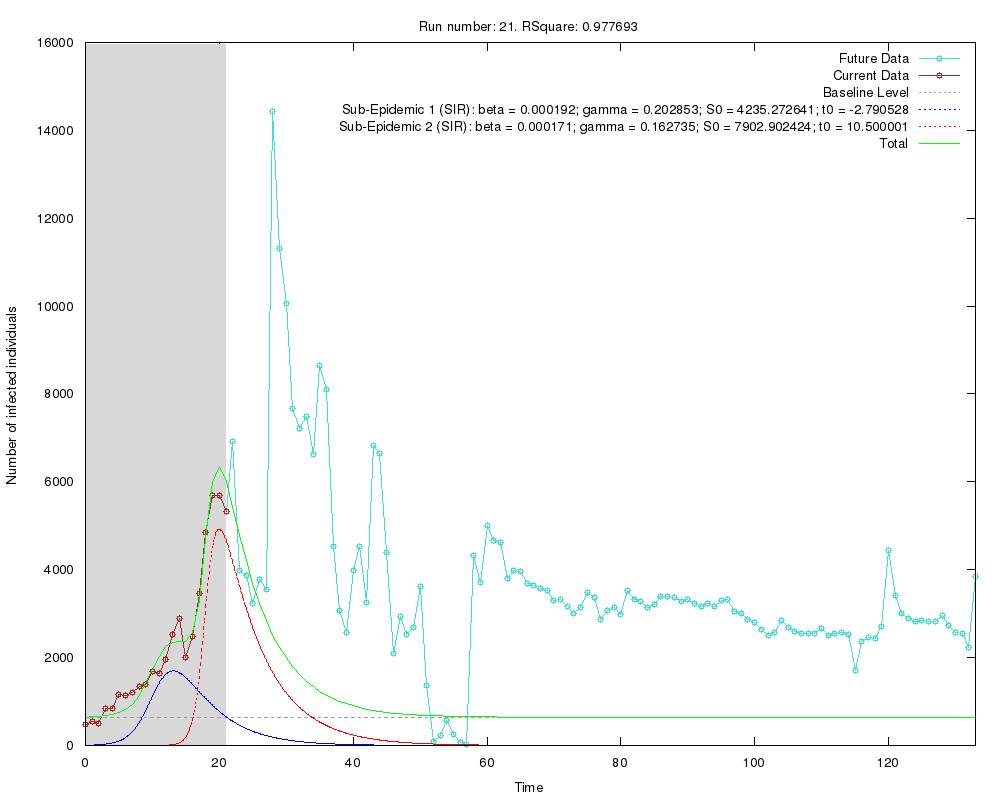
\includegraphics[width=8cm]{images/multi/goodrt1.png}
  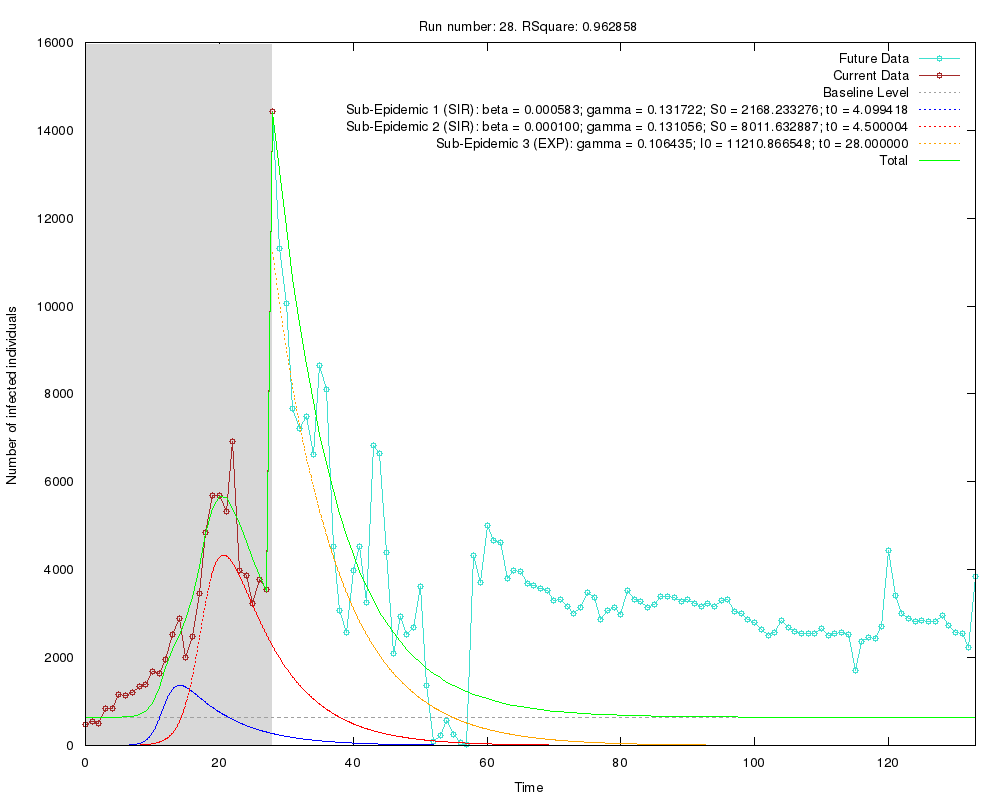
\includegraphics[width=8cm]{images/multi/goodrt2.png}
  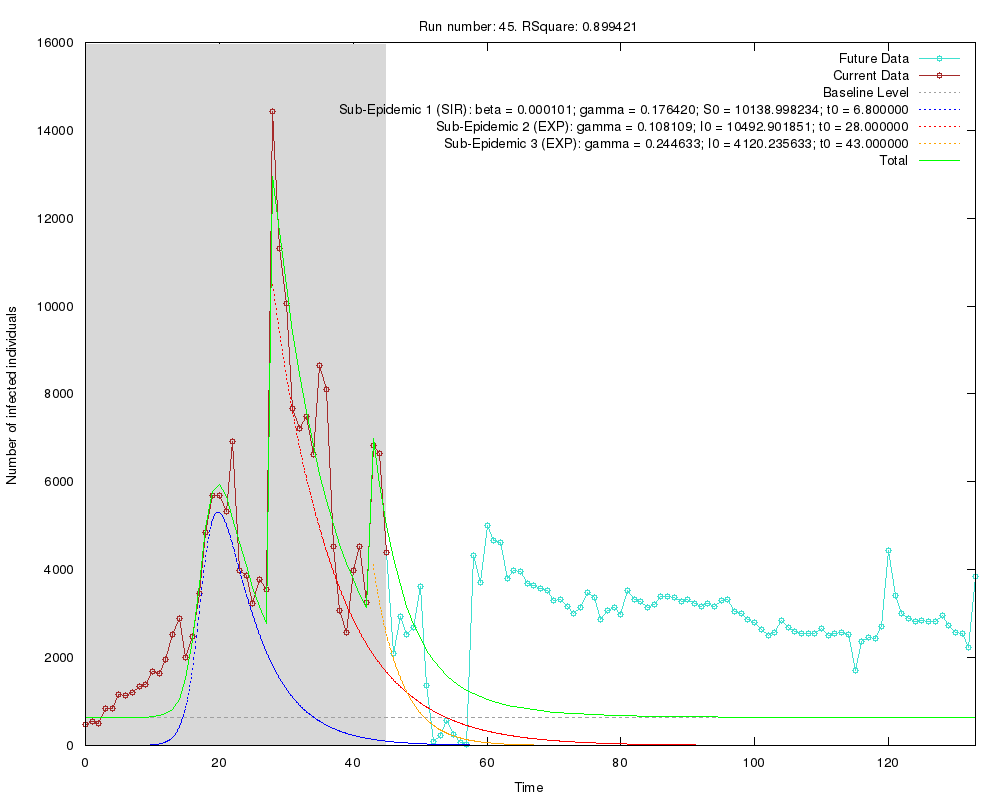
\includegraphics[width=8cm]{images/multi/goodrt3.png}
  \caption{Second multiple epidemic fitting procedure on ``Blurred
    Lines'' download data using additional logistic binding and
    modified Nelder-Mead algorithm }
\label{fig:goodrt}
  \end{figure}
\end{centering}

The updated implementation provides a much better fit throughout the
course of the run, and accurately locates the start of constituent
epidemics. Interestingly, these sub epidemics can be ascribed to real
world events that resulted in the sudden expose of ``Blurred
Lines''. The initial SIR shaped epidemic seems to be a result of the
initial video upload in March 2013. The second, larger spike epidemic
immediately follows the exposure of Robin Thicke on the US television
show, ``Jimmy Kimmel Live''. Another epidemic is detected at around
day 200, which coincides with the live performance of ``Blurred
Lines'' on the 2013 ``MTV Video Music Awards''. Finally, the final
epidemic at around day 250 immediately follows Robin Thicke's appearance on the TV show ``X Factor''.  



\section{Implementation Summary}
The model fitting framework proposed in figure~\ref{fig:uml} was
adapted to form the final synthedemic fitting framework. The flow of
control is summarised as follows:

\begin{enumerate}
\item An instance of the Datahandler class imports the desired
  epidemic data from a .csv file into a vector.
\item The Datahandler object begins the iterative fitting procedure
  with a target R Square value, as shown in \ref{fig:realtime}.
\item The fitting procedure starts with no epidemics, and attempts to
  find an optimal synthedemic model fit to the currently available
  data at each time point. This is done by passing the objective
  function in \ref{fig:objective} to an instance of the ``Nelder
  Mead'' class.
\item To prevent overfitting, the framework also attempts to optimise
  all possible $k-1$ epidemic combinations at each time point. If the
  resulting R Square value is above the threshold, the epidemic is
  permanently removed.
\item If the R Square value is below the desired threshold and a new
  epidemic outbreak has been detected, we
  consider adding each candidate model. We then choose to add the
  model with the lowest AICc score.
\item At the end of each time point, we plot the results of the
  optimisation and reset all temporary parameters.
\end{enumerate}

The Datahandler class stores a number of attributes that are used in the
optimisation procedure. For example, the currently avaiable data, the current best
fitting model and a vector of Epidemic objects. The reasoning behind
storing so many variables as properties rather than declaring them
locally is to speed up the optimisation procedure. The presented
implementation also uses logistic bounding on all parameters within a
sensible range to reduce the chance of the optimisation algorithm from
getting stuck in a bad local minima. The start time of each epidemic,
$t_0$ is also included in the optimisation procedure. By using
different bounds for each Epidemic sub class, we are able to limit the
parameter search space for each sub epidemic depending on the epidemic
type.

\begin{algorithm}
  \captionof{figure}{Synthedemic Fitting Framework Function}
  \begin{algorithmic}
    \Function{realtime\_model\_fit}{targetRSq, data} 
    \State //\emph{Begin the iterative procedure}
    \For{i = 0 to length(data)}
    \State //\emph{Get currently available data}
    \State availableData = data[1:i]\\
    \State //\emph{Optimise current set of $k$ epidemics to data}
    \State (optimParams, modelResults, RSquare, AICc) =
      optimiseEpidemics(availableData, epidemics)
      \\
      \If{RSquare \textgreater targetRSq}
      \For{j = 0 to length(epidemics)}
        \State tempEpidemics = fewer\_epidemics(j);\\
        \State //\emph{Optimise for $k-1$ epidemics}
        \State (tempParams, tempModel, tempRSquare, tempAICc) =
        optimiseEpidemics(availableData, tempEpidemics);\\
        \State //\emph{If fit sufficient, track this epidemic for removal}
        \If{tempAICc \textless AICc \& tempRSquare \textgreater
          targetRSq}
        \State //\emph{Store results for $k-1$ epidemics}
        \EndIf
        \State tempEpidemics = epidemics;
        \EndFor
        \EndIf
      \State remove\_epidemic(toRemove);
      \\
      \State //\emph{Check residuals for new outbreak}
      \State residuals = get\_residuals(availableData, modelResults);
      \State newEpidemic = check\_for\_epidemic();
   \\ 
   \State //\emph{If an epidemic was detected and the current fit is
     insufficient, attempt to add an epidemic}
   \If{newEpidemic != true \& RSquare \textless targetRSquare}
   \State tempEpidemics = epidemics;
   \\
   \State //\emph{Check the addition of each candidate model}
   \For{j = 0 to length(candidateModels)}
   \State tempEpi = newEpidemic(candidateModels[j]);
   \State tempEpidemics.push\_back(tempEpidemic);\\
   \State //\emph{Optimise for $k+1$ epidemics}
   \State (tempParams, tempResults, tempRSquare, tempAICc) = optimiseEpidemics(availableData, tempEpidemics);
   \If{tempAICc \textless AICc \& tempRSquare \textgreater
     targetRSq}
   \State toAdd = tempEpi;
   \State //\emph{Store results for $k+1$ epidemics}
   \EndIf
   \EndFor
   \EndIf\\
   \If{toAdd != NULL} epidemics.push\_back(toAdd); \EndIf
   \EndFor
   \EndFunction
  \end{algorithmic}
  \label{fig:realtime}
  \end{algorithm}

Note that at each time point that an epidemic is detected, we test the
model fit when each sub epidemic is removed. An alternative, simpler
approach would be to only consider removing the last epidemic at each
time point. Although this would improve the speed of the fitting
procedure, we risk leaving in superfluous sub epidemics from early on
in the fitting procedure. Including $t_0$ in the optimisation also
improves the ability of the remaining sub epidemics to compensate for
dropping an epidemic.

\begin{algorithm}
  \captionof{figure}{Epidemic Optimisation Function}
  \begin{algorithmic}
    \Function{optimise\_epidemics}{epidemics, availableData}
    \If{length(epidemics) == 0}
    \State model = baseline\_model(availableData);
    \State RSquare = calculate\_RSquare(model, availableData);
    \State AICc = calculate\_AICc(model, availableData);
    \State finalParams = ();
    \Else
    \State//\emph{Perform 10 random fits and choose best fitting run}
    \For{i = 0 to 10}
    \State seedParams = generate\_seed\_parameters();
    \State logit\_transform\_parameters(seedParams);
    \State (tempParams, tempSSE) = neldermead\_optim(*ode\_solve\_sse, seedParams);
    \If{tempSSE \textless SSE}
    \State SSE = tempSSE;
    \State finalParams = tempParams;
    \EndIf
    \EndFor
    \State model = ode\_solve(finalParams);
    \State AICc = calculate\_AICc(model, availableData);
    \State RSquare = calculate\_RSquare(model, availableData);
    \Return (finalParams, model, RSquare, AICc);
    \EndIf
    \EndFunction
  \end{algorithmic}
\label{fig:optimise}
\end{algorithm}


\begin{algorithm}
  \captionof{figure}{ODE Solving Function}
  \begin{algorithmic}
    \Function{ode\_solve}{parameters}
    \State total\_model = empty\_model
    \State total\_model = combine\_vectors(total\_model,baseline\_model);
    \State logistic\_transform\_parameters(parameters);
    \For{i = 0 to length(epidemics)}
    \State temp\_model = epidemics[i].ode\_solve(parameters);
    \State total\_model = combine\_vectors(total\_model,
    temp\_model);
    \EndFor
    \Return calculate\_sse(total\_model,current\_data);
    \EndFunction
    \end{algorithmic}
  \label{fig:objective}
\end{algorithm}
    
 Each Epidemic object also has its own set of ODEs. By calling the ``ode\_solve''
function for each Epidemic object separately, we are able to easily
include additional epidemic types without having to change the
optimisation framework. It should also be noted that different
candidate models require different logistic bounds. For example,
whereas the beta value of a typical \emph{SIR} model might lie in the
range of 0.0005 to 0.005, a typical beta value for an \emph{irSIR}
model is between 0.00001 and 0.0001. Again, by including using an
object oriented approach, we are able to bind the parameters of each
sub epidemic depending on its type. A final observation regarding
figure~\ref{fig:objective} is that it can easily be modified to return
the calculated model rather than the SSE value.

 

\chapter{Evaluation}
\label{ch:evaluation}



\chapter{Conclusion}

\label{ch:conclusions}

\section{Summary of Thesis Achievements}

Summary.


\section{Applications}

Applications.


\section{Future Work}

Future Work.

\appendix
% appendices come here


\addcontentsline{toc}{chapter}{Bibliography}
\bibliographystyle{alpha}
\bibliography{bibliography/bibliography}

\end{document}
